\documentclass[fontsize = 12pt, paper = a4]{scrreprt} 

\setlength{\parindent}{0pt}
\usepackage[english,ngerman]{babel}
\usepackage[utf8]{inputenc} 
\usepackage{enumerate}
\usepackage{amssymb,amsmath}

%------------ Überschriften verkleinern und hochsetzen ----------%

%\makeatlettern
%\renewcommand*\@makechapterhead[1]{%
%{\parindent \z@ \raggedright \normalfont
%\LARGE\bfseries
%\ifnum \c@secnumdepth >\m@ne
%\thechapter\space
%\fi
%#1\par\nobreak
%\vskip 20\p@
%}} 

% ------------------------ Blattlayout- -------------------------%

\usepackage {geometry}   
\geometry   {left     = 2.5cm,
             right    = 2.5cm, 
             top      = 1.5cm,
             bottom   = 1.5cm,
             includehead, includefoot}
             
% ------------------------ Seitenstil ---------------------------%           

% Umdefinieren von Befehlen zur Vermeidung von Bugs:

\renewcommand*{\chapterpagestyle}{scrheadings} 
\renewcommand*{\chapterheadstartvskip}{\vspace*{-\topskip}}

% Gestaltung der Kopf- und Fußzeile:

\pagenumbering{arabic}
            
\usepackage[automark]{scrpage2}
\automark[chapter]{section}
\pagestyle{scrheadings} 
\ohead[\pagemark]{\pagemark}
\setlength{\footskip}{5mm} 

\clearscrheadfoot
\lohead{Entwurfsdokument}
\rohead{\headmark}
\lofoot{Softwareprojekt TU Ilmenau SS 2013}
\rofoot{\pagemark}

% Kopf- und Fußzeilenlinie:

\setheadsepline{.6pt} % Linie für Kopfzeile
\setfootsepline{.6pt} % Linie für Fußzeile 

% Für Unterstreichungen:

\usepackage[normalem]{ulem}

% Buchstabenglättung am Rand:
  
\usepackage {microtype} 

% Bildunterschriften zentrieren:

\usepackage[center]{caption}

%-------------------------------------------------------------------%

% Für die Einbindung von Bildern:

\usepackage[pdftex]{graphicx} % .pdf, .png oder .jpg möglich!
\usepackage{rotating}         % Grafiken rotieren

% Nutzung in drei Umgebungen möglich:

% (1) \begin{turn}{Winkel} ...  \end{turn}
% (2) \begin{sideways} ... \end{sideways} 90° im math. pos. Sinn
% (3) \begin{rotate}{Winkel} ... \end{rotate} 
%     ---> 90° im math. pos. Sinn, allerdings keine Platzreservierung 

\usepackage{wrapfig}
%\usepackage{picins}   % Textumflossene Grafiken
\usepackage{subfigure}
\usepackage{floatflt}
\usepackage{float}
\usepackage[justification=centering]{caption}

%-------------------------------------------------------------------%
 
% Packete für Tabellen:

\usepackage{booktabs}
\usepackage{array}    % optional
\usepackage{tabularx} % optional

\usepackage[font=footnotesize,labelfont=bf,singlelinecheck=false,
            format=plain,,justification=justified,indention=0cm]                     {caption} 

\usepackage{setspace}
\usepackage{enumitem}
%% Unterstriche erlauben:
%
%\usepackage{underscore}


%----------------  Anfang des Dokuments ------------------%

\begin{document}

%*******************************************************************%

% Entwurf Titelseite:

\titlehead{\begin{center}
\textbf{\Huge Entwurfsdokument}
\end{center}}
		   
\title{Service-Interface \\ für ein Formula-Student-Fahrzeug}

\subtitle{Technische Universität Ilmenau \\
		  Softwareprojekt SS 2013 \\ Gruppe 19}			
		
\author{Christian Boxdörfer \\ Thomas Golda \\ Daniel Häger \\ 
		David Kudlek \\  Tom Porzig \\ Tino Tausch \\ 
		Tobias Zehner \\ Sebastian Zehnter}
		
\date{Hier Datum einfügen.}	 
	  
\publishers{betreut durch \\ \vspace{1cm} Dr. Heinz-Dietrich Wuttke, TU Ilmenau \\ Oliver Dittrich, fachlicher Betreuer Team StarCraft e.V.}

\maketitle		

%*******************************************************************%

% --------------------- Inhaltsverzeichnis -----------------------%

\begin{spacing}{0.86} 
\tableofcontents
%\setcounter{secnumdepth}{4} % Tiefere Gliederungsebene  
\setcounter{tocdepth}{4} % Anzeige bis Gliederungsstufe 4
%\addtocontents{toc}{\protect\enlargethispage{2\baselineskip}} 
\end{spacing}


\newpage % Seitenumbruch

%--------------------------  Einleitung  ---------------------------%

\chapter{Einleitung}

Dieses Entwurfsdokument für das Service-Interface des Formula-Student-Fahrzeugs bündelt Feinentwurf und Entwicklerdokumentation.
Es ist daher in drei größere Kapitel untergliedert, die zuerst den Feinentwurf des Softwaresystems behandeln. Hierzu werden vor allem Modellierungen der einzelnen Komponenten des Softwarepakets mit UML aufgezeigt und erläutert.
Im Anschluss wird auf die Änderungen zum Grobentwurf hinsichtlich der letzten Phase des Projekts aufgezeigt und gerechtfertigt. Schließlich wird auf ausgewählte Implementierungsabschnitte detailliert eingegangen und diese erläutert.
Jedes dieser drei Kapitel ist dabei weiter unterteilt in die Abschnitte MicroAutoBoxII, Embedded PC und Webseite. Dabei umfasst der Teil Embedded PC auch das auf dem vServer laufende Programm zum Empfangen der Daten und Einfügen derselben in die Datenbank, da diese beiden Programme sich sehr ähneln und auch essentiell viele gleiche Klassen benutzen. Das Löschen veralteter Daten auf dem vServer, welches durch ein eigenständiges Programm realisiert wird, wird jeweils im Unterkapitel vServer abgehandelt. Die Unterteilung der Kapitel entspricht also auch den einzelnen Stationen, auf denen Teile unseres Softwarepakets laufen. Die genannte Reihenfolge orientiert sich dabei am Fluss der Daten, wie sie ihren Weg von der MicroAutoBoxII über den Embedded PC und das auf dem vServer laufende Programm zur Webseite zurücklegen.

%--------------------------  Feinentwurf  --------------------------%

\chapter{Feinentwurf}

%------------------------- MicroAutoBox II -------------------------%

\section{MicroAutoBox II}

\subsection{Verwendete Blöcke - Ergänzungen}

Um den späteren Nutzern des Service-Interfaces den Einstieg in das erzeugte Modell in Simulink anhand konkreter Modellausschnitte zu erleichtern, wurden bereits die für den Grobentwurf benötigten Blöcke im Entwurfsdokument unter 3.2.1 vorgestellt. Jedoch ist es aufgrund mehrerer obligatorischer Anpassungen während der Implementierung des Feinentwurfs notwendig geworden, gegenüber dem Grobentwurf auf eine größere Vielfalt an Blöcken zurückzugreifen. Aus diesem Grund wird nun im Folgenden die jeweilige Funktionalität der erstmalig verwendeten Blöcke erläutert.

\subsubsection{Math Operations}

\begin{itemize}

\begin{figure}[h]
\centering
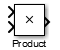
\includegraphics[scale = 1]{product}
\caption[Produkt-Block]{Produkt-Block zur Multiplikation zweier Signale}
\label{Produkt-Block}
\end{figure}

\item[1)] \textit{Produkt-Block}

Durch den Produkt-Block wird es ermöglicht, zwei Eingangssignale miteinander zu multiplizieren und das entstehende Ausgangssignal im Signalfluss weiterzuführen. In diesem Modell wird dieser Block dazu verwendet, mithilfe des Width-Blockes (Verweis) die exakte Größe eines UDP-Paketes für einen bestimmten Datentyp (Verweis)zu berechnen. Darüber hinaus bietet dieser gegenüber dem Gain-Block bessere Laufzeiteigenschaften, wobei diesem vorteilhaften Aspekt oft eine größere Anzahl an zu verwendenden Blöcken und Leitungen gegenübersteht.

\end{itemize}


\subsubsection{Logic and Bit Operations}

\begin{itemize}

\begin{figure}[h]
\centering
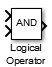
\includegraphics[scale = 1]{and}
\caption[UND-Gatter]{UND-Gatter}
\label{UND-Gatter}
\end{figure}

\newpage

\item[1)] \textit{UND-Gatter}

Dieser Block bildet als logischer Operator die exakte Funktionsweise eines UND-Gatters nach. Sollten an diesem Block die bis zur einer Anzahl \textit{n} anschließbaren Eingangssignale mit dem Datentyp \textit{boolean} allesamt als booleschen Werte eine logische 1 oder allesamt eine logische 0 aufweisen, so liegt am Ausgang des Blocks eine logische Eins an, andernfalls wird bei unterschiedlichen booleschen Werten am Ausgang eine 0 ausgegeben.  

\end{itemize}


\subsubsection{Signal Attributes}

\begin{itemize}

\begin{figure}[h]
  \centering
\begin{minipage}[b]{3cm}
    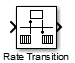
\includegraphics[scale = 0.85]{rate_transition}
    \caption[Rate-Transition-Block]{Rate-Transition-Block}
  \end{minipage}
\hspace*{3cm}  
  \begin{minipage}[b]{3 cm}
    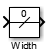
\includegraphics[scale = 0.9]{width}
    \caption[Width - Block]{Width - Block}     
  \end{minipage}
\end{figure}

\item[1)] \textit{Rate-Transition-Block}

Der Rate-Transition-Block bietet die Möglichkeit, Signale vom Output des Blockes, welche mit einer unterschiedlichen Frequenz als der Input des Blockes arbeiten, an den Input anzugleichen. Dieser Block wird oftmals benötigt, wenn zwei verschiedene Signale unterschiedliche "`Sample Times" aufweisen die nicht manuell durch Änderung einer Sample Time aneinander angeglichen werden können. Innerhalb des Blockes stehen mehrere Optionen zur Verfügung, welche die Integrität der Daten und die Latenzzeiten der Signale beeinflussen. In unserem Falle wurden zur Sicherstellung der korrekten Angleichung bzw. der korrekten Weiterleitung der Signale die beiden Optionen "`Ensure data integrity during data transfer"\ und "`Ensure deterministic data transfer (maximum delay)"\ ausgewählt, was gegenüber den dadurch erzielten Vorteilen eine vertretbare Erhöhung der Latenzzeiten zur Folge hat. 

\item[2)] \textit{Width-Block}

Der Width-Block ermittelt wie sein Name schon vermuten lässt die Breite des anliegenden Input-Signals und leitet diese an den Output weiter. Hierbei können an den Input sowohl Vektoren als auch Busarrays angeschlossen werden. \\
Folgende Datentypen werden hierbei unterstützt: 

\begin{itemize}

\item Floating point
\item Built-in integer
\item Fixed point
\item Boolean
\item Enumerated

\end{itemize}

(Quelle: http://www.mathworks.de/de/help/simulink/blocklist.html) 

\end{itemize}

\newpage


\subsubsection{Signal Routing}

\begin{itemize}

\begin{figure}[h]
\centering
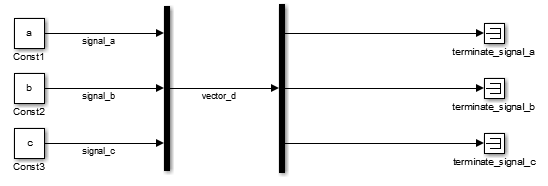
\includegraphics[scale = 1]{mux_demux}
\caption[Multiplexer / Demultiplexer]{Modell zur Erläuterung eines Multiplexers / Demultiplexers}
\label{Multiplexer / Demultiplexer}
\end{figure}

\item[1)] \textit{Multiplexer}

Analog zum Bus Creator (s. Entwurfsdokument S.10) besitzt auch der Multiplexer die Fähigkeit, mehrere Eingangssignale zum einem einzelnen Signal zu bündeln. Jedoch besteht zwischen den beiden Komponenten ein gravierender Unterschied: während beim Busarray die einzelnen Eingangssignale weiterhin individuell vorliegen und demzufolge nur virtuell gebündelt werden um die Übersichtlichkeit innerhalb des Modells zu erhöhen, werden die Signale beim Multiplexer zu einem reellen Signalvektor zusammengefasst (s. Abb. \ref{Multiplexer / Demultiplexer}). In diesem Beispiel werden die durch die drei Constant-Blöcke Const1-Const3 erzeugten Werte \textit{a}, \textit{b} und \textit{c} zu dem Signalvektor \textit{vector\_d} zusammengefasst, welcher nun die folgende Gestalt besitzt: 

\vspace*{2mm}

\begin{centering}

$ vector\_d = \left( \begin{array}{c} signal\_a \ signal\_b \ signal\_c \end{array} \right)^{T}$

\end{centering}

\vspace*{-2mm}


\item[2)] \textit{Demultiplexer}

Mit dem Demultiplexer ist es anschließend möglich, aus dem Inputsignal \textit{vector\_d} bestimmte Elemente zu entnehmen und auszugeben. In diesem Beispiels werden die drei Elemente des Vektors jeweils wieder einzeln als Skalare herausgeführt und anschließend auf Terminator-Blöcke geleitet. Je nach Anzahl der Inputs \textit{n} und der Outputs \textit{p} des Demultiplexers ergeben sich u.a. die folgenden Kombinationen:

\end{itemize}

\vspace*{-6mm}

\begin{table}[h]
\centering

\caption{Funktionsweise des Demultiplexers}

 \begin{tabular}{ c | c }
 
 \toprule[1.5pt]
 \textbf{Anzahl der Parameter} & \textbf{Ausgabe des Blockes} \\ 
 
 \midrule
 $n = p$    & $p$ skalare Signale   \\
 $p > n$    & Fehlermeldung       \\
 $p < n$ , $n\ mod\ p = 0$ & $p$ Signalvektoren mit $\frac{n}{p}$ Elementen \\
 $p < n$ , $n\ mod\ p = m$ & $m$ Vektorsignale mit $\frac{n}{p}+1$ Elementen \\
    & und $(p-m)$ Signale mit $\frac{n}{p}$ Elementen   \\ 
  
 \bottomrule[1.5pt]
 
\end{tabular}

\end{table}
 
\vspace{\baselineskip}

\vspace*{-8mm}


\begin{centering}
(Quelle: http://www.mathworks.de/de/help/simulink/slref/demux.html)
\end{centering}
\newpage


\subsubsection{Simulink Extras}

\begin{itemize}

\begin{figure}[h]
\centering
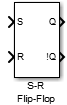
\includegraphics[scale = 0.8]{flipflop}
\caption[S-R-Flip-Flop]{S-R-Flip-Flop}
\label{S-R-Flip-Flop}
\end{figure}

\item[1)] \textit {S-R-Flip-Flop}

Dieser Block bildet die Funktionsweise eine S-R-Flip-Flops nach, welches die folgende bekannte Wertetabelle besitzt:

\begin{table}[h]
\centering

\caption{Wertetabelle S-R-Flip-Flop}

 \begin{tabular}{ c | c | c | c}
 
 \toprule[1.5pt]
 S (Set) & R (Reset) &  $Q_{n}$ & $!Q_{n}$ \\
 \midrule
  0 & 0 & $Q_{n-1}$ & $!Q_{n-1}$ \\
\midrule  
  0 & 1 & 0 & 1 \\
\midrule  
  1 & 0 & 1 & 0 \\
\midrule  
  1 & 1 & 0 & 0 \\
 
 \bottomrule[1.5pt] 
 
\end{tabular}

\end{table}

Hierbei ist zu beachten, dass an den beiden Eingängen S (Set) und R (Reset) vom Datentyp \textit{boolean} niemals gleichzeitig zwei logische Einsen anliegen dürfen, die Eingangsbelegung $[1,1]$ stellt somit eine verbotene Eingangsbelegung dar.  

\end{itemize}


\subsubsection{dSPACE-Blöcke}

\begin{itemize}

\item[1)] \textit{UDP-Receive-Block}

\begin{figure}[h]
\centering
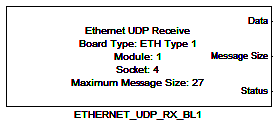
\includegraphics[scale = 0.8]{eth_udp_rx}
\caption[UDP-Receive]{UDP-Receive-Block}
\label{UDP-Receive}
\end{figure}

Mittels des UDP-Receive Blockes wird es der MicroAutoBox II ermöglicht, vom Embedded-PC einen Datenstrom vom Datentyp \textit{uint32} zu empfangen. Dies ist notwendig, um einerseits durch 
den Embedded-PC das zu versendende Datenpaket der MicroAutoBox II auszuwählen und andererseits den Grundstein einer bidirektionalen Kommunikation zwischen den beiden bereits genannten Komponenten für spätere Erweiterungen des Service-Interfaces durch externe Personen zu legen.

\newpage

\item[2)] \textit{Decode32-Block}

\begin{figure}[h]
\centering
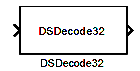
\includegraphics[scale = 0.8]{decode32}
\caption[DSDecode32-Block]{Block zur Dekodierung eines \textit{uni32}-Datenstromes}
\label{UDP-Receive}
\end{figure}

Der Dekoder-Block DSDecode32 stellt das passende Gegenstück zu dem Enkoder-Block DSEncode32 dar und basiert ebenfalls wie die dieser auf einer sFunction der Firma dSPACE. Er hat die Aufgabe, den empfangenen Datenstrom zu dekodieren und in einem Signalvektor in dem gewünschten Datentyp (Verweis) auszugeben. 

\item[3)] \textit{Byte-to-8bit-Dekoder}

\begin{figure}[h]
\centering
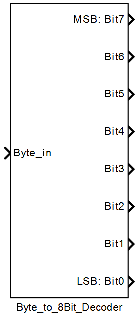
\includegraphics[scale = 0.8]{byteto8bit}
\caption[Byte-to-8-bit-Dekoder]{Byte-to-8-bit-Dekoder}
\label{Byte-to-8-bit-Dekoder}
\end{figure}

Bei dem Byte-to-8-bit-Dekoder handelt es sich um einen weiteren Block, der auf einer sFunction basiert. Durch ihn wird es ermöglicht, aus einem Byte Daten die einzelnen Bits zu isolieren und diese getrennt an den Outputs weiterzuleiten.

\end{itemize}



%--------------------------------------------------------------------%

\subsection{Config-Dateien}

\subsubsection{signalgenerator\_microautbox.m}

Wie schon im Entwurfsdokument beschrieben, dient diese *.m-File dazu, eine übersichtliche Darstellung über die Werteverläufe aller im Signalgenerator (Verweis) erzeugten Testsignale zu gewährleisten und eine eventuelle Modifikation ebendieser durch eine ausführliche Kommentierung so komfortabel wie möglich zu gestalten. Des Weiteren wurde um die Benennung der Parameter in dieser Config-Datei zu vereinfachen jeder Funktionsvektor mit dem Präfix "`SIGNAL\_"\ und jeder Zeitvektor mit dem Präfix "`TIME\_"\ versehen. Die korrekte Referenzierung dieser Vektoren in Constant- (Verweis) oder RSI-Blöcken (Verweis) ist dem Entwurfsdokument aus Abbildung 3.21 zu entnehmen.  

\subsubsection{config\_datenpaket.m}

Dieses *.m-File beinhaltet drei Vektoren, welche für den Embedded-PC erforderlichen Informationen über das zu  versendende Datenpaket mit den Fahrzeugdaten beinhalteten. Diese drei Vektoren werden jeweils in einem Constant-Block (Verweis) referenziert und bilden mit anderen Paketinformationen das zu versendende "`Informationspaket"\, welches vor dem eigentlichen Start der Datenübertragung an den Embedded-PC übertragen wird. Der maßgebliche Grund für das Anlegen dieses Config-Files war es, dem Nutzer eine eventuelle Modifikation des Simulink-Modells zu vereinfachen und zusätzlich auf dem Embedded-PC ein hohes Maß an Softcoding zu realisieren, was den Anpassungsaufwand des dort ausgeführten C++ - Programms bei derartigen Veränderungen drastisch reduziert. Im Folgenden soll nun der Zweck der einzelnen Vektoren erläutert werden. \\

1) VEKTOR\_AUFTEILUNG\_DATENPAKET  \\  

Dieser Vektor beschreibt, an welchen Stellen des Datenpaketes welche Datentypen anliegen, um anschließend auf dem Embedded-PC entsprechende Optimierungen bei der Umrechnung/Kovertierung der Daten und die Aufteilung des Datenpaketes anhand der einzelnen Gruppen A) - E) (s. Pflichtenheft) vornehmen zu können. Dieser $1 \times N$ - Zeilenvektor mit aktuell $N = 401$ Fahrzeugwerten wird aus Aspekten der Benutzerfreundlichkeit aus einer $N \times 3$ - Matrix namens MATRIX\_AUFTEILUNG\_DATENPAKET erzeugt, wobei die einzelnen Spalten für die folgenden Einträge stehen: 

\begin{center}
[ Start | Stop | Datentyp ]
\end{center}

Hierbei ist jeder verwendete Datentyp analog zu den sFunctions \textit{DSEncode32} und \\ \textit{DSDecode32} (Verweis) mit einer Ziffer kodiert:

\vspace*{-3mm}

\begin{table}[h]

\caption{Kodierung der Datentypen}

\begin{tabular}{ c | c | c | c | c | c | c | c | c | c}
 
\toprule[1.5pt]
\textbf{Datentyp} & \textit{boolean} & \textit{int8} & \textit{uint8} & \textit{int16} & \textit{uint16} & \textit{int32} & \textit{uint32} & \textit{float} & \textit{double}  \\ 

\midrule

\textbf{Ziffer} & 1 & 2 & 3 & 4 & 5 & 6 & 7 & 8 & 9  \\

\bottomrule[1.5pt] 
 
\end{tabular}

\end{table}

So gibt - um ein Beispiel anzuführen - "`1 4 3"\ in einer Zeile der Matrix an, dass die ersten vier Elemente des Datenpaketes den Datentyp \textit{unit8} besitzen. Diese Matrix wird nun mittels einiger Befehle in den oben aufgeführten Vektor umgewandelt und somit an das C++ - Programm auf dem Embedded-PC korrekt angepasst. Dies geschieht beispielhaft auf folgende Weise: So wird laut der obigen Bildungsvorschrift bei einer Matrix der Form der Zeilenvektor V mit den Einträgen der jeweiligen Datentypen der Elemente 1-4 erzeugt: 

\vspace*{4mm}

$ M = \left( \begin{array}{c} 1 \ 2 \ 3 \\ 3 \ 4 \ 5 \end{array} \right)$

\vspace*{4mm}

$ V = \left( \begin{array}{c} 3 \ 3 \ 5 \ 5  \end{array} \right)$

\newpage
 

2) VEKTOR\_PAKETTEILUNG \\

Dieser Vektor enthält als Elemente diejenigen Stellen, bei denen eine Aufteilung der einzelnen Datengruppen der Fahrzeugdaten in die Kategorien A) -- E) erfolgt(s. Pflichtenheft). X $\mid$ Y  in der Kommentaren der *.m-File gibt an, zwischen welchen Stellen das Datenpaket im C++ -- Programm getrennt werden muss. Dies verfolgt den Zweck, das auf dem Embedded-PC empfangene Datenpaket in fünf Datenpakete mit den jeweiligen Datengruppen aufzuteilen, um einerseits eine klarere Zuordnung der Daten auf dem vServer zu ermöglichen und andererseits eventuell auftretenden Verbindungsproblemen und einbrechenden Signalstärken bei der Übertragung via UMTS an den vServer zu begegnen. \\

3) VEKTOR\_KOMMASETZUNG \\

Dieser Vektor $1 \times N$ - Zeilenvektor mit $N = 401$ Fahrzeugdaten  liefert Informationen darüber, bei welchen Daten bzw. bei 
welchen Elementen das Komma um eine bestimmte Anzahl von Stellen nach links verschoben werden muss (0:= Keine Stelle, 1:= Um eine Stelle nach links verschieben etc.).

%--------  Aufbau des Simulink-Modells -- Signalgenerator  ---------%

\subsection{Aufbau des Simulink-Modells -- Signalgenerator}

\subsubsection{Gesamtaufbau}

\begin{figure}[h]
\centering
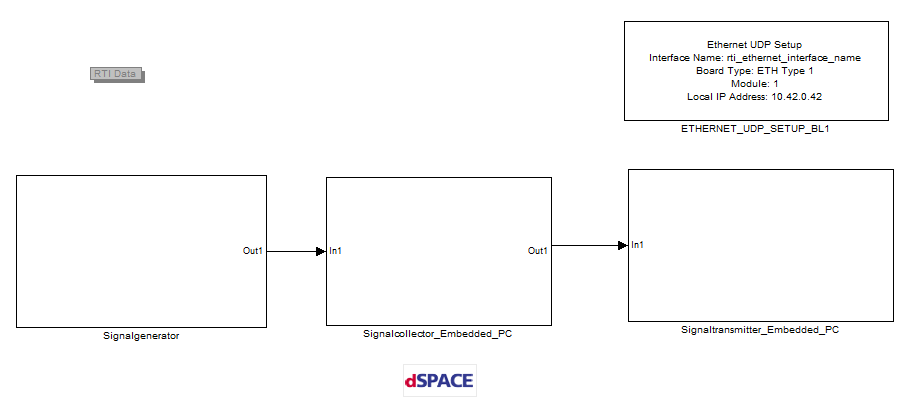
\includegraphics[scale = 0.65]{topmodell}
\caption[Gesamtaufbau Simulink-Modell]{Gesamtaufbau des Simulink-Modells auf höchster Modellebene}
\label{topmodell}
\end{figure}

\newpage

Wie in Abbildung \ref{topmodell} dargestellt, unterteilt sich der Aufbau des Simulink-Modells in drei übergeordnete Subsysteme: 

\begin{itemize}

\item Signalgenerator
\item Signalkollektor
\item Signaltransmitter

\end{itemize}

wobei der Signalgenerator den Beginn und der Signaltransmitter das Ende des Signalflusses verkörpert. Des Weiteren ist es auch notwendig, sowohl die Maske RTI\_DATA\_HOST (Verweis Glossar) als auch den UDP-Setup-Block (s. Entwurfsdokument S. 12) auf der obersten Ebene des Simulink-Modells zu platzieren. Im Folgenden soll nun detailliert auf die einzelnen Komponenten und der jeweiligen Funktionalität dieser drei Subsysteme eingegangen werden. 



\subsubsection{Signalgenerator}


Der Signalgenerator hat die Aufgabe auf der MicroAutoBox II die für einen Systemtest benötigten Testsignale zu generieren, welche zuerst zum Signalcollector (s. 2.1.4) und anschließend über den  Signaltransmitter (s. 2.1.5)  auf den Embedded-PC via Ethernet-Schnittstelle gelangen und daraufhin über eine GPRS/UMTS-Verbindung an einen virtuellen Server gesendet werden. Diese Signale liegen im Bereich der echten Sensorwerte des Fahrzeuges und können somit gut zu Testzwecken verwendet werden. Da sich eine Modifizierung des in der MicroAutoBox II implementierten Simulink-Modells als sehr aufwändig gestaltet, ist die Generierung der Testsignale enorm wichtig, um die Funktionalität des Simulink-Modells und letztendlich auch des Service-Interfaces zu überprüfen. Vor der Implementierung des finalen Simulink-Modells wird dieser Teil des Modells von einem Mitglied von Team StarCraft e.V. durch eine Verknüpfung zu den realen Sensorwerten, welche vom CAN-Bus des Fahrzeuges geliefert werden, ersetzt. \\

\textit{Aufbau} \\

Wie im Pflichtenheft aufgeführt, sind die Signale der Fahrzeugdaten in die fünf verschiedene Gruppen A) -- E) namens \textit{Allgemeine Fahrzeugdaten}, \textit{Akkudaten}, \textit{dynamische Daten}, \textit{Fahrdynamikregelung} sowie \textit{Motor- und Umrichterdaten} unterteilt. Diese Gliederung wurde im Signalgenerator ebenfalls beibehalten um ein hohes Maß an Übersichtlichkeit und Modularität zu gewährleisten. Der Signalgenerator ist demnach nochmals in einzelne Subsysteme unterteilt, welche die verschiedenen Kategorien der jeweiligen Fahrzeugdaten repräsentieren. Die generierten Signale werden über einen \textit{Bus Creator} (s.Entwurfsdokument S.10) in ein Bussignal (Verweis Vektorsignal / Bussignal zu meinem Text) umgewandelt und gebündelt über diesen Bus an den Signalkollektor übermittelt, wobei die Reihenfolge der eingehenden Daten erhalten bleibt. \\

Innerhalb der einzelnen Subsysteme werden nun die simulierten Fahrzeugdaten generiert. Ein Subsystem ist hierbei eine Bündelung mehrerer Blöcke und Komponenten, welche auch wiederum Subsysteme sein können. Dies hat den Zweck, die Übersichtlichkeit innerhalb des Gesamtmodells zu wahren. Weiterhin kann ein solches Subsystem problemlos mehrfach verwendet werden, was den Aufwand beim Erstellen des Modells erheblich reduzieren kann. Am Beispiel \textit{Allgemeine Fahrzeugdaten} soll nun ohne Beschränkung der Allgemeinheit der Aufbau eines Subsystem im Signalgenerator näher erläutert werden.


\begin{figure}
\centering
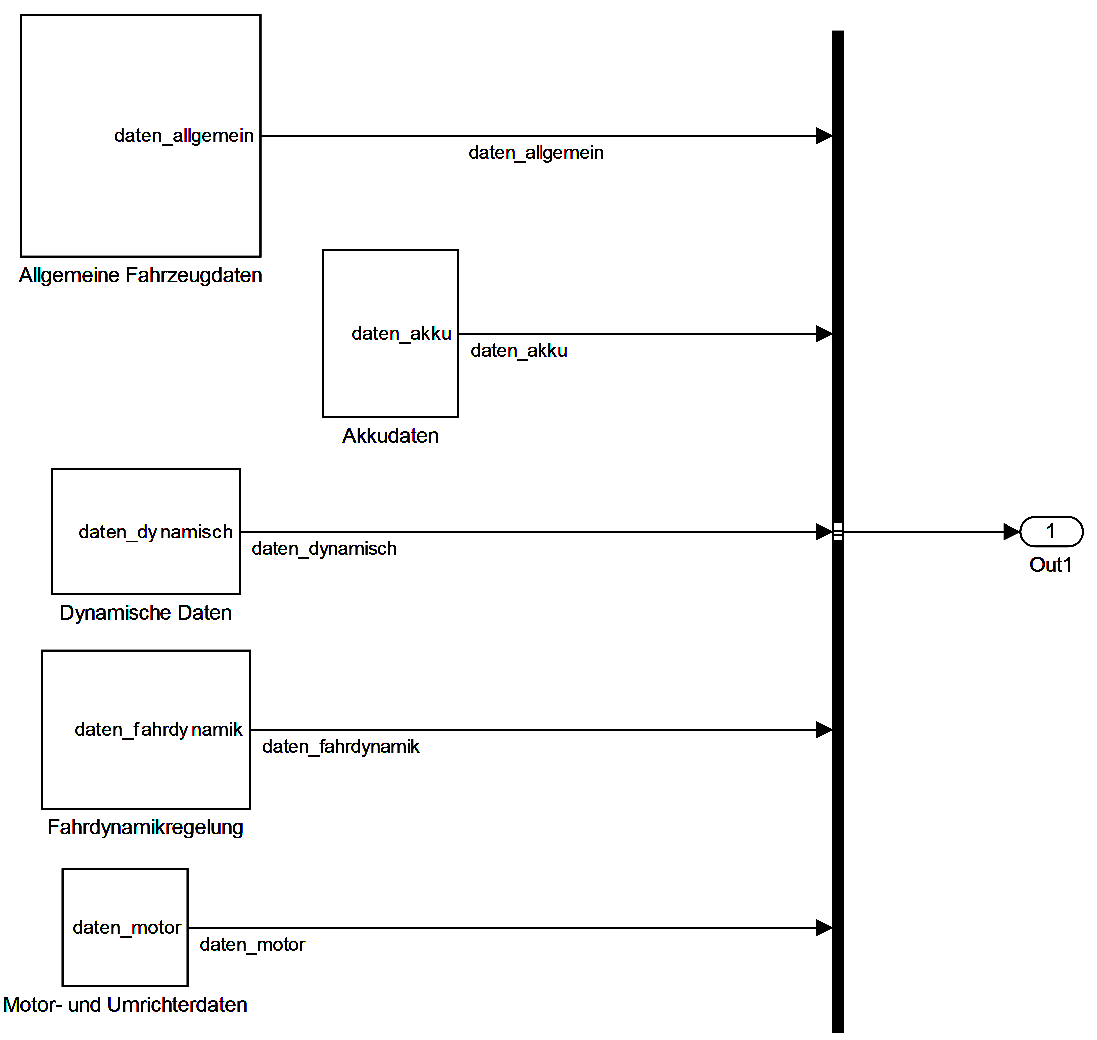
\includegraphics[scale = 0.4]{sub_signalgenerator}
\caption[Subsysteme des Signalgenerators]{Unterteilung des Signalgenerators in die einzelnen Subsysteme}
\label{sub_signalgenerator}
\end{figure}


\begin{figure}
\centering
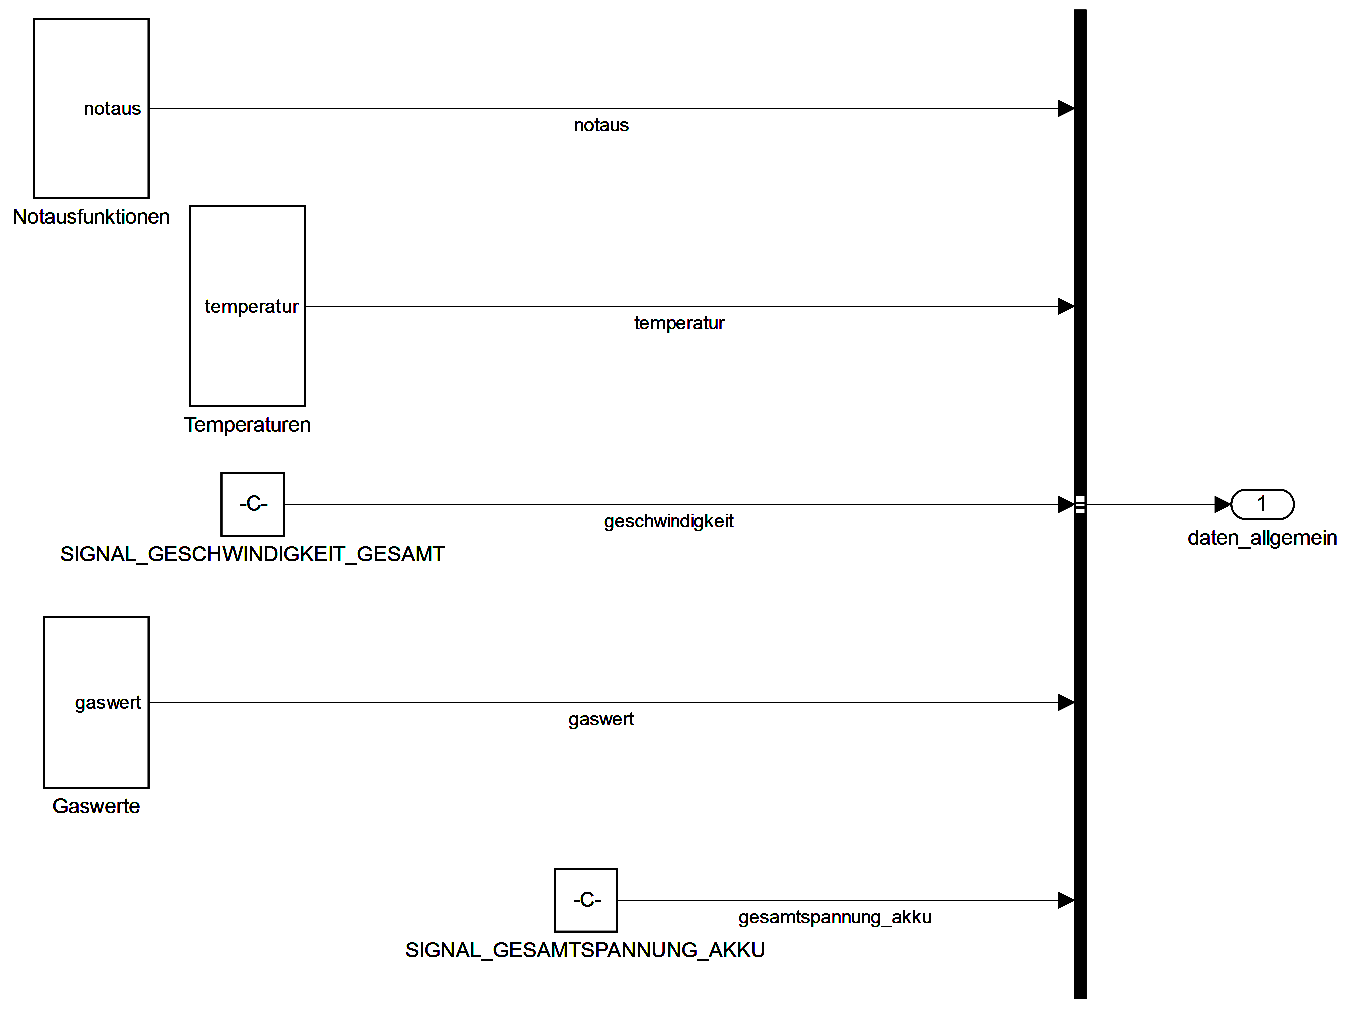
\includegraphics[scale = 0.37]{daten_allgemein}
\caption[Subsysteme Allgemeine Fahrzeugdaten]{Aufbau des Subsystems    Allgemeine Fahrzeugdaten}
\label{Allgemeine Fahrzeugdaten}
\end{figure}

\newpage




Wie in Abbildung \ref{Allgemeine Fahrzeugdaten} zu sehen ist, beinhaltet das Subsystem \textit{Allgemeine Fahrzeugdaten} selbst einige Subsysteme sowie andere Simulinkblöcke. Weiterhin befinden sich im Subsystem \textit{Allgemeine Fahrzeugdaten} weitere Subsysteme mit den Namen Notausfunktionen, Temperaturen und Gaswerte. Jedes Subsystem hat eine unterste Ebene in welcher keine Subsysteme mehr vorhanden sind. Weiterhin werden die einzelnen Signale innerhalb eines Subsystems mittels des bekannten Bus Creators zur einem Bussignal gebündelt. Das hat den Sinn, dass das gesamte Subsystem nur einen Output besitzt, was das ganze Modell wesentlich übersichtlicher  gestaltet und hierdurch einfacher du handhaben ist. \\

\textit{Erzeugung der einzelnen Signale } \\

\textit{A) Allgemeine Fahrzeugdaten} \\

\begin{figure}[h]
\centering
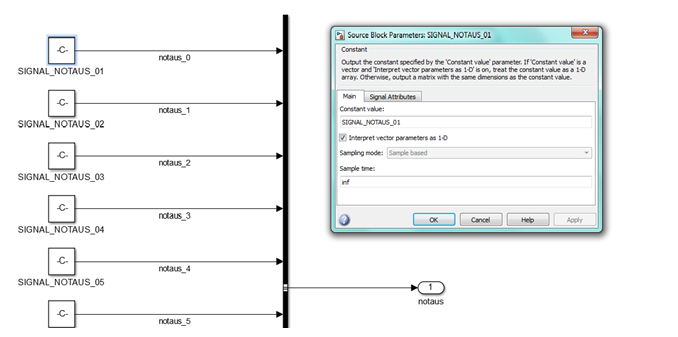
\includegraphics[scale = 0.95]{notaus}
\caption[Testsignale der Notaus-Schalter]{Erzeugung und Referenzierung der Notaus-Schalter im Simulink-Modell}
\label{notaus}
\end{figure}

Die Notaussignale, welche die Zustände der einzelnen Notausschalter des Fahrzeuges symbolisieren, werden über die Constant-Blöcke(s. ED S.8) erzeugt. Sie besitzen den Datentyp \textit{boolean} und die Parameterwerte werden über das *.m-File \textit{signalgenerator.m},  zuerst diese in den Workspace von Matlab schreibt, von dort referenziert, um die Handhabung des Modells zu erleichtern(s. 2.1.2). Dabei ist SIGNAL\_NOTAUS\_01 der Variablenname, welcher dem System aufgrund des *.m-Files bekannt ist und  direkt aus dem Workspace  ausgelesen wird. Dieses Signal wird über einen Bus Creator mit den anderen Signalen des Subsystems zu einem Signal gebündelt und an das Subsystem \textit{Allgemeine Fahrzeugdaten} mit dem Variablennamen "`notaus"\ übergeben. Im Subsystem \textit{Allgemeine Fahrzeugdaten} wird dieser Output wiederum mit den restlichen Signalen über einen Bus Creator zur einem Ausgabewert mit dem Namen "`daten\_allgemein"\ zusammengefasst.  Im Subsystem Signalgenerator  werden diese Daten letztendlich mit den restlichen generierten Fahrzeugdaten über einen weiteren Bus Creator gebündelt und an den Signalkollektor übergeben. 

\newpage

Dies geschieht analog mit den weiteren Notaussignalen. Die Temperaturen handhaben sich auf die gleiche Weise wie die Notaussignale, wobei der einzige Unterschied dabei in dem jeweilig verwendeten Datentyp besteht. Da die Datentypen im weiteren Verlauf noch mehrfach konvertiert werden(s. SC, ST), spielt er bei der Erzeugung keine Rolle. Somit wird er vom Constant-Block durch die Einstellung "`Inherit: Inherit from Constant value"(s. \ref{constdatentyp}) selbst festgelegt. Der Parameter "`Gesamtgeschwindigkeit"\ wird auch in einem Constant-Block generiert. Dieses befindet sich jedoch nicht nochmals in einem Subsystem, da es nur ein Wert dieser Art ist. Somit liegt er direkt an dem Bus Creator des \textit{Allgemeine Fahrzeugdaten} Subsystems an. Schließlich verhalten sich die Parameter Gaswerte äquivalent zu den Temperatursignalen und der Parameter  "`Gesamtspannung Akku"\ handhabt sich wie die Gesamtgeschwindigkeit.


\begin{figure}[h]
\centering
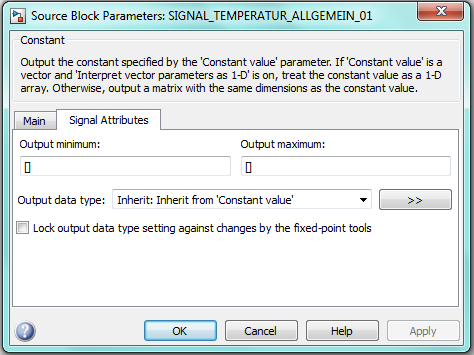
\includegraphics[scale = 0.8]{const_datentyp}
\caption[Enstellungen zum Datentyp im Constant-Block ]{Einstellungen zum verwendeten Datentyp im Constant-Block}
\label{constdatentyp}
\end{figure}

\textit{B) Akkudaten} \\

Die Signalerzeugung im Subsystem \textit{Akkudaten} verläuft ähnlich wie im Subsystem \textit{Allgemeine Fahrzeugdaten}. Das Subsystem ist für die Generierung folgender Signale verantwortlich: Die Zellspannungen(Zelldaten) der Akkus, deren Temperaturen, die maximale sowie minimale Zellspannung, die Gesamtspannung der Akkus, der Ladestrom, die Ladespannung und die Zustände des Balancings (s. Abb. \ref{akkudaten}). \\

Die Zelldaten werden über einen "`Repeating Sequence Interpolated"\ -- Block(s. ED S.9) erzeugt. Äquivalent zu den \textit{Allgemeinen Fahrzeugdaten} werden auch hier die Parameterwerte, in diesem Fall SIGNAL\_ZP\_01\_ZELLE\_01, durch Variablen aus dem Config-File signalgenerator\_microautobox.m referenziert, wo diese hinterlegt sind (s. Abb. \ref{makezelldaten}). Weiterhin gibt bei diesem Block die Variable im Feld "`Vector of time values"\ Auskunft darüber, zu welchen diskreten Zeiten sich der Ausgabewert dieses Blockes ändert. Auch dieser Wert(in diesem Fall "`TIME\_08") ist in der oben genannten *.m-File  definiert (s. 2.1.2). Eine Sample time 0.01 bedeutet, dass der Wert alle 0.01 Sekunden abgetastet wird. 

\newpage

Diese Sample time von 0.01 wird im ganzen Modell bei den "`Repeating Sequence Interpolated" -- Blöcken verwendet. Nach der Erzeugung des Wertes "`zelle\_001"\ wird dieser mittels Bus Creator mit den anderen Werten seines Subsystems gebündelt und als Output "`zellenpack\_01"\ aus dem Subsystem Zellenpack\_01 ausgegeben.

\begin{figure}[h]
\centering
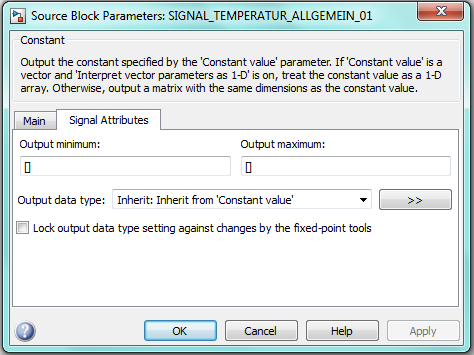
\includegraphics[scale = 0.8]{const_datentyp}
\caption[Enstellungen zum Datentyp im Constant-Block ]{Einstellungen zum verwendeten Datentyp im Constant-Block}
\label{constdatentyp}
\end{figure}


\begin{figure}[h]
\centering
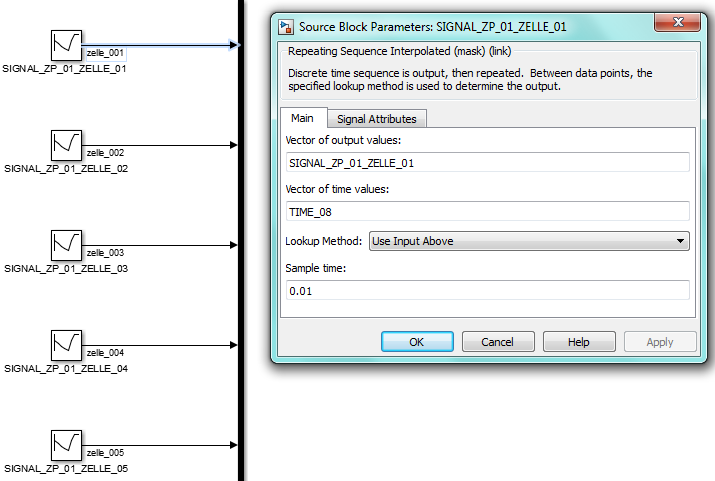
\includegraphics[scale = 0.65]{makezelldaten}
\caption[Generierung der Zelldaten]{Erzeugung der Zelldaten über einen RSI-Block mittels eines Signal- und eines Zeitvektors}
\label{makezelldaten}
\end{figure}

\newpage

Das übergeordnete Subsystem "`Zelldaten"\  beinhaltet abermals weitere zwölf Subsysteme namens "`Zellpack\_01"\ bis "`Zellpack\_12" (s. Abb. \ref{zelldaten}). Es werden dort nach den Vorgaben des Pflichtenheftes 144 Zelldaten erzeugt, von denen sich jeweils zwölf Zellen in einem Zellenblock befinden. Aus diesem Grund bietet es sich zur Erhöhung der Übersichtlichkeit an, die Signalgenerierung innerhalb der zwölf Subsysteme vorzunehmen. Im Subsystem "`Zelldaten" wird das Signal "`zellenpack\_01"\ mit den Signalen der anderen zwölf Subsysteme gebündelt und mit den Variablenname "`zelldaten" an das Subsystem "`Akkudaten"\  ausgegeben. An dieser Stelle werden die Signale des kompletten Subsystems wiederholt mit einem Bus Creator gebündelt und als "`daten\_akku"\ an das Subsystem \textit{Signalgenerator} übergeben. Danach werden wie bei dem Subsystem "`Allgemeine Fahrzeugdaten"\ erläutert alle Signale zusammengefasst und an den Signalkollektor übertragen, wobei diese Prozedur für alle Zelldaten gleichermaßen abläuft. \\

Die Signalerzeugung der Akkutemperaturen verläuft analog zu den Zelldaten. Die einzigen Unterschiede sind, dass nur vier Temperaturen pro Zellenpack existieren und der Zeitvektor Wert sich auf "`TIME\_10" bezieht (s. 2.1.2). Die maximale sowie minimale Zellspannung, der Ladestrom sowie die Ladespannung werden direkt mittels "`Repeating Sequence Interpolated" -- Blöcken im Subsystem \textit{Akkudaten} erzeugt und auch direkt in diesem über den Bus Creator mit den anderen Signalen gebündelt. Der Wert für den Zeitvektor beläuft sich bei ihnen auf "`TIME\_08". Die Gesamtspannung verhält sich hierzu weitestgehend  gleich, allerdings wird sie durch einen Constant-Block generiert. Die Balancingdaten werden i.A. äquivalent zu den Zelldaten aufbereitet, da zu jeder Zelle ein Balancing Wert gehört. Nur allein die Signalerzeugung ist anders, da die Werte des Balancings mit Hilfe eines Constant-Blockes in dem Datentyp \textit{boolean} erstellt werden. \\

\textit{C) Dynamische Daten} \\

Das Subsystem \textit{Dynamische Daten} ist für die Erzeugung folgender Signale zuständig \\ (s. Abb. \ref{dyndaten}) : Geschwindigkeit, Beschleunigung, Gierrate, Drehzahlen der Räder, Wassertemperatur, Bremsdruck, Bremskraft, Bremsposition, Federweg, Gaspedalstellung und Lenkwinkel. Alle Signale werden mittels "`Repeating Sequence Interpolated" -- Blöcken und der Einstellung "`TIME\_08"\ für den  Wert Zeitvektors generiert, wobei die Werte der einzelnen Signale im *.m-File signalgenerator\_microautobox.m (s. 2.1.2) definiert sind. \\

Das Signal "`geschw1" wird im Subsystem \textit{Geschwindigkeit} erzeugt und mit den anderen Daten im Subsystem über einen Bus Creator gebündelt und als Signal "`geschw" an das Subsystem \textit{Dynamische Daten} übergeben, wo es dort mit den anderen Werten wieder mittels Bus Creator gebündelt wird. Das entstandene Signal "`daten\_dynamisch" wird im Subsystem \textit{Signalgenerator} wieder mit den restlichen Signalen bzw. Subsystemen gebündelt und an den \textit{Signalkollektor} geschickt.

\newpage

\begin{figure}[h]
\centering
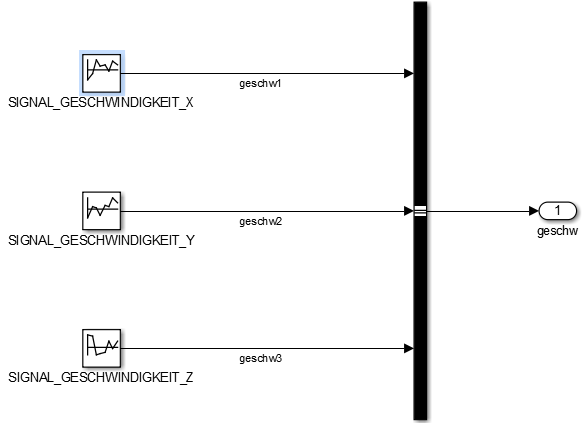
\includegraphics[scale = 0.85]{makegeschwindigkeit}
\caption[Generierung der Testsignale für die Geschwindigkeit des Fahrzeuges]{Erzeugung der Testsignale über die Geschwindigkeit des Fahrzeuges in X- , Y- und Z-Richtung mittels dreier RSI-Blöcke}
\label{makegeschwindigkeit}
\end{figure}

Die Subsysteme \textit{Beschleunigung}, \textit{Gierrate}, \textit{Drehzahlen der Räder}, \textit{Wassertemperatur}, \textit{Federweg} sowie \textit{Gaspedalstellung} verhalten sich absolut äquivalent zu den Geschwindigkeitssignalen.
Der Verlauf der Signale "`Bremsdruck", "`Bremskraft"\ und "`Bremsposition" verhält sich -- bis auf deren Erzeugung bereits im Subsystem \textit{Dynamische Daten} -- absolut gleich. \\

\textit{D) Fahrdynamikregelung} \\

Das Subsystem \textit{Fahrdynamikregelung} ist für die Erzeugung der Testsignale "`Antriebsschlupfregelung"\ und "`Torque Vectoring" verantwortlich (s. Abb. \ref{makefahrdynamik}). Diese werden mit RSI-Blöcken gebildet, welche die gleiche Konfiguration wie bei dem Subsystem \textit{Dynamischen Daten} besitzen. Beide Werte werden jeweils im Subsystem selbst erzeugt und über den Bus Creator gebündelt als Signal "`daten\_dynamisch" an das Subsystem \textit{Signalgenerator} übergeben, wobei der weitere Signalverlauf äquivalent zu den anderen Signalen in ebendiesem Subsystem ist.

\newpage

\begin{figure}[h]
\centering
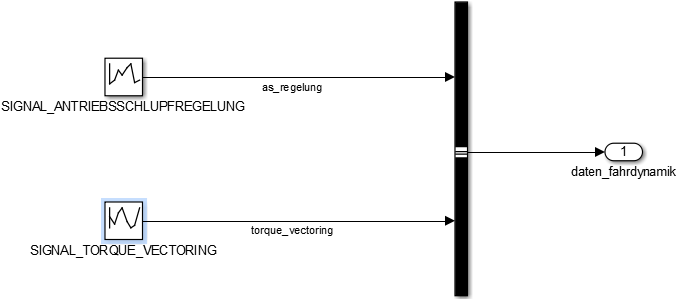
\includegraphics[scale = 0.75]{makefahrdynamik}
\caption[Generierung der Testsignale für die Fahrdynamik des Fahrzeuges]{Erzeugung der Testsignale für die Fahrdynamik des Fahrzeuges mittels zweier RSI-Blöcke}
\label{makefahrdynamik}
\end{figure}

\textit{E) Motor- und Umrichterdaten} \\

Im Subsystem \textit{Motor- und Umrichterdaten} werden die Signale "`DC Strom", "`DC Spannung", "`Motortemperatur", "`Stromgrenze", "`Maximalleistung", "`Lüfterdrehzahl", "`Lüfter", "`Pumpe"\ sowie die Wassertemperatur des Motors erzeugt (s. Abb. \ref{submotordaten}). Alle Signale werden erneut mit Hilfe von RSI-Blöcken generiert. Die Konfiguration dieser Blöcke gleicht denen des Subsystems \textit{Dynamische Daten}. Die Signalaufbereitung ist bei allen Signalen äquivalent. Allein die Signale der Motortemperatur werden in einem eigenen Subsystem \textit{Motortemperatur} und nicht direkt im Subsystem \textit{Motor- und Umrichterdaten} erzeugt. Es findet auch wieder eine Bündelung der Signale mittels eines Bus Creator statt und und das gebündelte Signal "`daten\_motor" wird an das Subsystem \textit{Signalgenerator} übergeben. Der weitere Signalverlauf ist äquivalent zu den anderen Signalen im Subsystem \textit{Signalgenerator}.


\subsection{Signalkollektor}

Der Signalkollektor stellt das zweite große Subsystem innerhalb des Simulink-Modells dar. Er hat die Aufgabe, den vom Subsystem \textit{Signalgenerator}(s. 2.1.3) oder von einem späteren Subsystem von Team StarCraft e.V. erhaltenen Busarray wieder in die einzelnen Signale zu unterteilen, geeignet aufzubereiten und diese dann an den \textit{Signaltransmitter}(s. 2.1.5) weiterzuleiten, welcher die erzeugten Testsignale bzw. Sensordaten an den Embedded-PC via Ethernet-Schnittstelle sendet. Während der Aufbereitung der Signale im Signalkollektor werden die folgenden Schritte durchgeführt:

\begin{itemize}

\item[1)] \textit{Verstärkung der Signale}

Abhängig von der Anzahl der Nachkommastellen des Testsignals $n$ mit $n > 0$ wird dieses nun durch einen Gain-Block (s. ED S.11) mit dem Faktor $10^n$ multipliziert, um für den aktuellen Wert des Testsignals jeweils einen ganzzahligen Wert zu erhalten,
was zur Vereinheitlichung der zu übertragenden Daten beitragen soll.

\newpage

\item[2)] \textit{Konvertierung der Datentypen}

Die nunmehr ganzzahligen Werte werden von ihren Datentypen \textit{boolean} oder \textit{single} nun einheitlich mittels eines Convert-Blocks in den Datentyp \textit{int16} konvertiert, wodurch alle Signale den gleichen Datentyp aufweisen. Schließlich ist noch eine Konvertierung in den Datentyp \textit{double} vonnöten, da die sFunction \textit{DSEncode32} (s. ED S.12) diesen Datentyp voraussetzt. Allerdings liefert diese sFunction als Ausgabe erneut den Datentyp \textit{int16}, weshalb die vorherige Konvertierung am Eingang der sFunction nicht ins Gewicht fällt.  

\item[3)] \textit{Umbenennung der Variablennamen}

Mit dem Convert-Block ist es zudem möglich, dem Ausgangssignal unabhängig vom Eingangssignal einen festen bzw. neuen Variablennamen zu vergeben. Dies ist insofern nützlich, da bei einem möglichen Zugriff auf die Daten bzw. die Variablen durch
den Embedded-PC oder der Software Control Desk von dSPACE diese immer die gleichen Variablennamen besitzen, unabhängig davon ob der Signalgenerator durch das Subsystem von Team StarCraft e.V. ersetzt
wurde oder nicht, wodurch eine Vereinheitlichung des Modells realisiert wird welche die Wartungsaufgaben erleichtert.

\end{itemize}

Nachdem die Daten entsprechend der obigen Schritte aufbereitet wurden, werden diese erneut durch mehrere Bus Creator und Subsysteme auf einem zentralen Bus Creator zu einem Busarray gebündelt und  an einen Encoder (s. ED S.12) übergeben, woraufhin sie nach deren Enkodierung via Ethernet-Schnittstelle an den Embedded-PC versendet werden. \\

%-------------------------------------------------------------------%

\textit{Aufbau} \\

Die Daten liegen wie bereits in Abschnitt 2.1.3 erläutert am Eingang des Subsystems "`Signalkollektor\_Embedded\_PC"\ an. Um ebendiese effizient und übersichtlich bearbeiten zu können, muss dieser Busarray wieder in seine einzelnen Signale zerlegt werden. Hierfür wird der Busarray zuerst mittels eines Bus Selectors (s. ED S.10) wieder in die fünf bekannten Hauptkategorien Allgemeine Fahrzeugdaten, Akkudaten, Dynamische Daten, Fahrdynamikregelung sowie Motor- und Umrichterdaten aufgespalten. Diese werden dann anschließend in ihren Subsystemen weiterverarbeitet und aufgespalten. Schlussendlich werden alle Signale erneut gebündelt und mit Hilfe von Bus Creators durch einen Convert-Block in den Datentyp \textit{double} konvertiert, um diese für die sFunction DSEncode32 passend vorzubereiten (s. Abb. \ref{subsignalkollektor}). Im Folgenden sollen daher nun der Aufbau und die Funktionsweise der einzelnen Subsysteme innerhalb des Subsystems "`Signalkollektor\_Embedded\_PC"\ dargelegt werden. \\

%-------------------------------------------------------------------%

\textit{Subsystem daten\_allgemein / Allgemeine Fahrzeugdaten} \\

Wie in ABB2 ersichtlich besteht auch dieses Subsystem aus mehreren Subsystemen sowie Simulink-Blöcken. Am Subsystem selbst liegen die Signale als Input vor, wie diese aus dem dazugehörigen Subsystem des Signalgenerators ausgegeben wurden. Diese werden durch einen Bus Selector wieder einzeln aufgetrennt.

\newpage

Die Signale "`gesamtspannung\_akku"\ und "`geschwindigkeit"\ werden mittels des Gain-Blocks um den Faktor 10 vergrößert, um die eine Kommastelle zu beseitigen, damit diese bei der int16-Konvertierung im Convert-Block nicht verloren geht. Zuzüglich generiert der Convert-Block einen festen Variablennamen, welche für den Rest des Simulink-Modells gilt. Üblicherweise wird dem normalen Variablennamen vor Konvertierung noch der Präfix "`emb"\ hinzugefügt bzw. "`daten" durch "`emb"\ ersetzt. So geht aus "`gesamtspannung\_akku"\ der neue Signalname "`emb\_gesamtspannung\_akku"\ hervor. Diese Umwandlung der Variablennamen wird auch innerhalb der Subsysteme nach der Bündelung mit dem Bus Creator vorgenommen. Aus "`daten\_notaus"\ entsteht der neue Variablenname "`emb\_notaus". Das Signal "`emb\_gesamtspannung\_akku"\ wird durch einen Bus Creator mit den anderen Signalen seines Subsystems erneut gebündelt und mit dem Variablennamen "`emb\_daten\_allgemein"\ an das Subsystem "`Signalcollector\_Embedded\_PC"\ übergeben. Dort wird diese Kategorie an Signalen erneut mit den anderen Signalen zu einem Busarray zusammengefügt, per Convert-Block in den Datentyp \textit{double} umgewandelt, um es für die Enkodierung aufzubereiten. Schlussendlich werden diese Daten an den Signaltransmitter versandt. 

\begin{figure}[h]
\centering
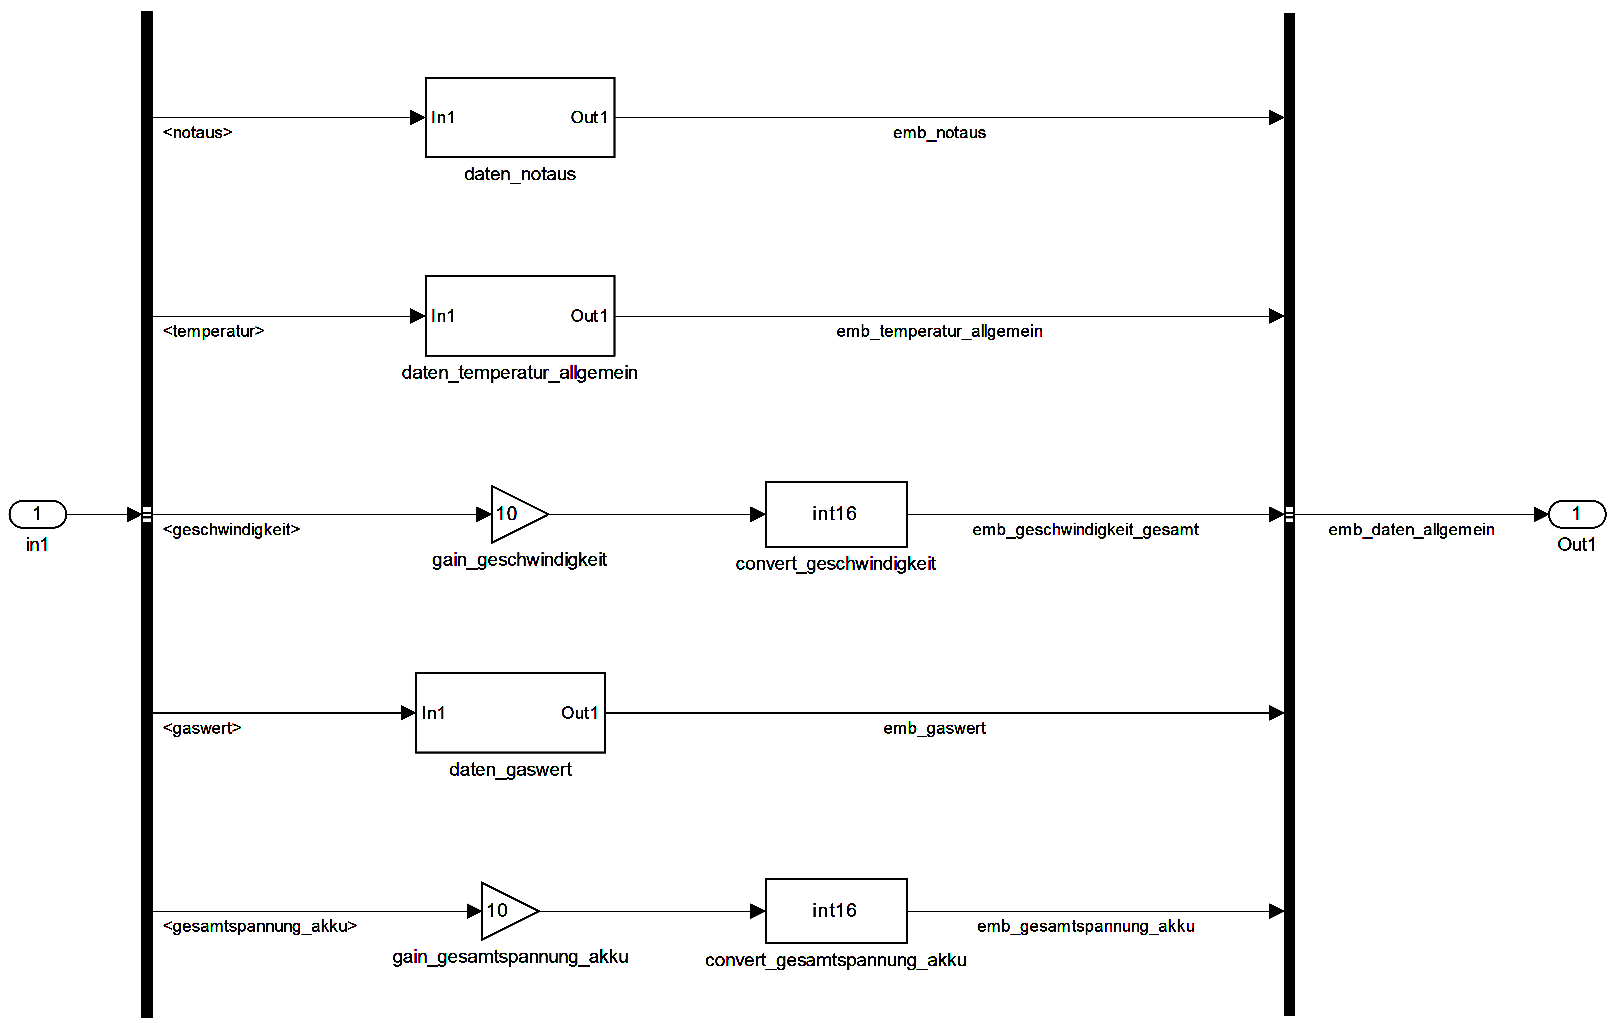
\includegraphics[scale = 0.37]{sc_daten_allgemein}
\caption[Übersicht über Subsystem "`daten\_allgemein"\ im Signalkollektor]{Übersicht über das Subsystem "`daten\_allgemein"\ im Signalkollektor}
\label{scdatenallgemein}
\end{figure}

Des Weiteren wird das Subsystem \textit{daten\_notaus} ohne Beschränkung der Allgemeinheit betrachtet (s. Abb. \ref{scdatennotaus}). Innerhalb des Subsystems wird das Busarray mittels eines Bus Selectors in die einzelnen Signale aufgegliedert. Das Signal "`notaus\_0" wird mittels eines Convert-Blockes in den Datentypen \textit{int16} konvertiert und erhält den neuen Variablennamen "`emb\_notaus\_01". Als Rundungsmethode für \textit{boolean} Werte wurde "`Floor" gewählt, da diese auf ganze Zahlen rundet. Dies ist nur logisch, da aus "`true"\ und "`false", eine logische 1 und eine logische 0 resultieren soll.

\newpage

Danach bündelt ein Bus Creator dieses Signal mit den anderen seines Subsystems und übergibt die Daten an das Subsystem \textit{daten\_allgemein} mit dem Variablenname "`emb\_notaus" (s. ABB3). Anschließend werden die Daten wie oben erläutern weiter verarbeitet(Umbennung des Busarray, Bündelung, Konvertierung und Transfer an Signaltransmitter). Die anderen Signale des Subsystems werden äquivalent aufbereitet. Dieses Vorgehen wird in diesem Modell bei allen boolean Werten im Signalkollektor angewendet. \\

Zur Verdeutlichung des Unterschieds von boolean und nicht-boolean Werten wird zusätzlich als Beispiel das Subsystem \textit{daten\_temperatur\_allgemein} betrachtet. Die Auftrennung der Signale mittels Bus Selector sowie die Umbenennung durch den Convert-Block gleichen dem Vorgehen des Subsystems \textit{daten\_notaus}. Differierend dazu sind die Multiplikation der Werte mittels Gain-Blöcke und die Rundungsmethode. Diese Unterschiede erschließen sich aus dem vorherrschenden Datentyp, welcher nicht \textit{boolean} ist. Wie schon oben betrachtet werden die Signale mittels Gain-Block um den Faktor 10 vergrößert, um die Kommastelle verschwinden zu lassen, damit die Genauigkeit des Wertes durch den Convert-Block bei der Konvertierung in den Datentyp \textit{int16} nicht beeinträchtigt wird. Weiterhin wird die Rundungsmethode "`Round" verwendet, welche den bekannten geodätischen Runden entspricht und eine zufriedenstellende Genauigkeit liefert. (s. Abb. \ref{scdatentemperaturallgemein}). Die restliche Aufbereitung bis hin zum Transferieren der Werte gleicht dem oben beschriebenen Vorgehen. Dieses Vorgehen wird in diesem Modell bei allen Werten welche nicht den Datentyp \textit{boolean} aufweisen im Signalkollektor angewendet, abgesehen natürlich vom Gain-Block, dessen Multiplikator je nach Anzahl der erforderlichen Kommastellen unterschiedlich sein kann. Die Verarbeitung der Signale im Subsystem \textit{daten\_gaswert} verlaufen hierzu äquivalent. Der einzige Unterschied dabei ist, dass die Verstärkung des Gain-Blockes 1000 beträgt, da bei diesen Werten eine Genauigkeit von drei Kommastellen vorgegeben ist (s. Pflichtenheft S.4) und diese Kommastellen mit der Vergrößerung beseitigt werden. \\

%-------------------------------------------------------------------%


\textit{Subsystem "`daten\_akku" / Akkudaten} \\

Wie im letzten Kapitel erwähnt (s. Subsystem "`daten\_allgemein"), verhalten sich alle Subsysteme im Signalkollektor sehr ähnlich. Es existieren in diesem Subsystem zwei Subsysteme, "`daten\_zelldaten"\ sowie "`daten\_temperatur", welche sich um die Verarbeitung von Werten kümmern, welche nicht den Datentypen \textit{boolean} aufweisen. Darüber hinaus existiert noch ein Subsystem mit boolean-Werten -- "`daten\_balancing"\ -- und einzelne Signale, welche ebenfalls Werte verkörpern, die nicht den Datentyp \textit{boolean} besitzen. Wie erwähnt findet auch eine Signalkonvertierung, eine Umbenennung der Variablennamen, sowie teilweise eine Verstärkung der Signale mittels Gain-Blöcken statt. Die weitere Signalaufbereitung im Subsystem \textit{Signalcollector\_Embedded\_PC} entspricht der des Subsystemes \textit{daten\_allgemein} (s. letzten Abschnitt). Die Verarbeitung der Signale, welche sich nicht nochmals in einem Subsystem befinden, gleicht der aus dem vorherigen Abschnitt. Einzig die Faktoren des Verstärkung der Signale "`zellspannung\_max"\ und "`zellspannung\_min"\ sind aufgrund der vorgegebenen Genauigkeit (s. Pflichtenheft S.4) in diesem Fall zu 1000 gewählt.

\newpage

\begin{figure}[h]
\centering
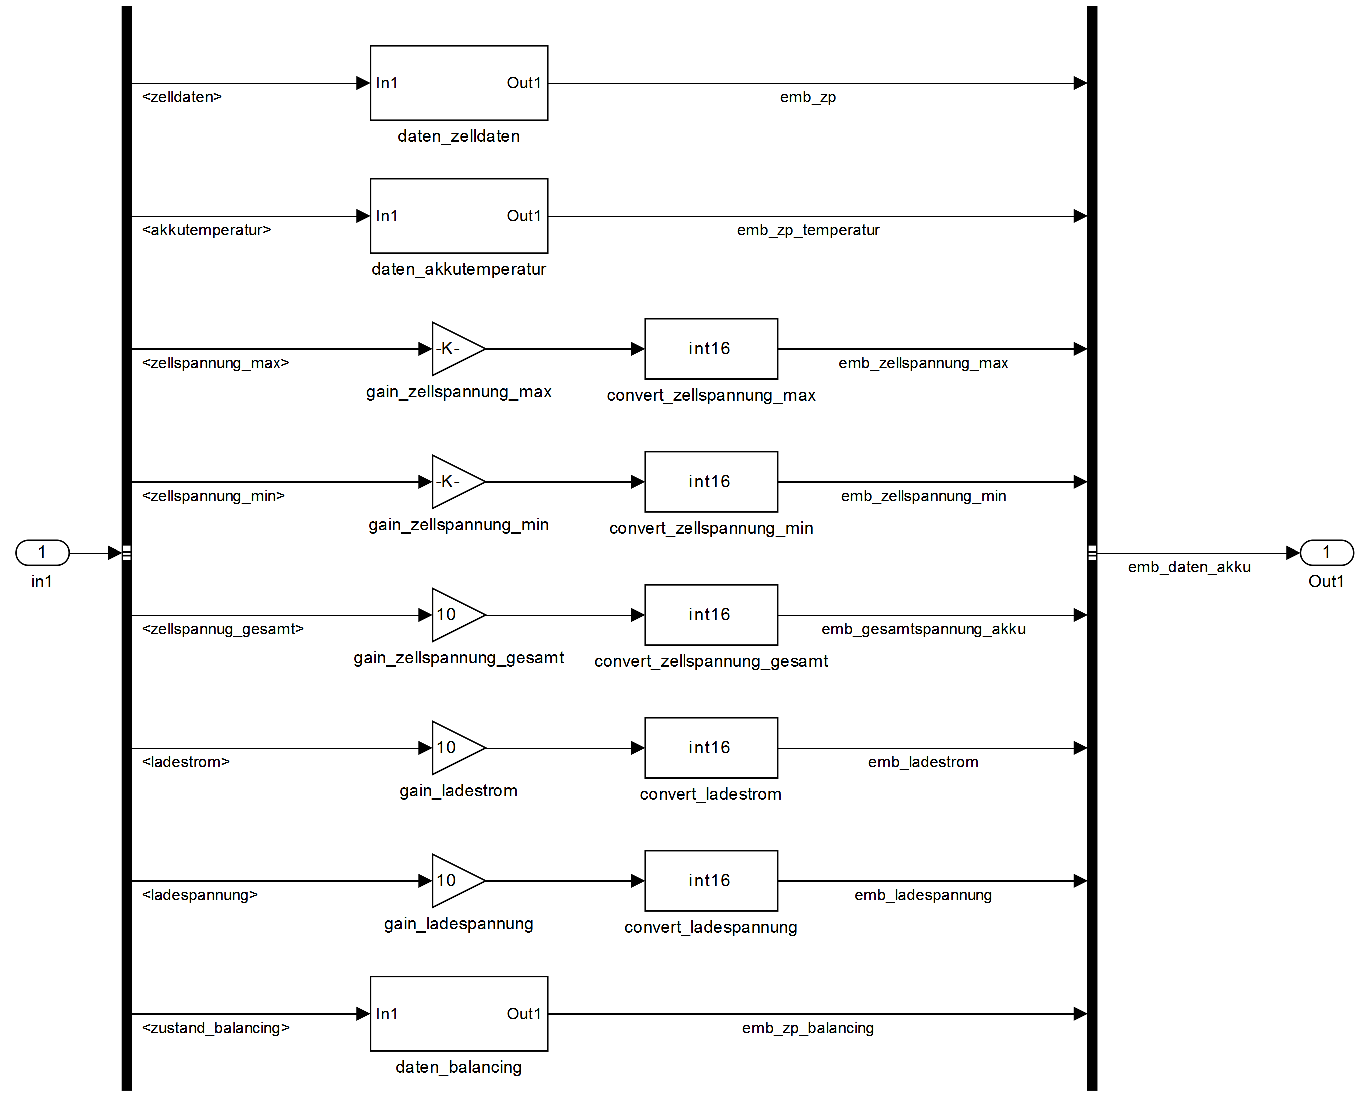
\includegraphics[scale = 0.45]{sc_daten_akku}
\caption[Übersicht über das Subsystem "`daten\_akku"\ im Signalkollektor]{Übersicht über das Subsystem "`daten\_akku"\ im Signalkollektor}
\label{scdatenakku}
\end{figure}

Die Subsystemstruktur soll anhand des Subsystems \textit{"`daten\_zelldaten"} (s. Abb. \ref{scdatenzellenpack}) ohne Beschränkung der Allgemeinheit kurz näher erläutert werden. Ähnlich wie im dazugehörigen Subsystem aus dem Signalgenerator (s. 2.1.3) ist auch dieses System aufgebaut. Das Signal "`zelle\_001"\ im Subsystem \textit{"`daten\_zellenpack\_01"} des Subsystems \textit{"`daten\_zelldaten"} wird mit einem Multiplikator von 1000 durch den Gain-Block versehen und mittels Convert-Block in den Datentyp \textit{int16} umgewandelt und in "`emb\_zp\_01\_zelle01"\ umbenannt. Dabei kann die Zelle jeweils genau einem Zellenpack zugeordnet werden. Anschließend wird das Signal mit dem Bus Creator mit den restlichen Signalen seines Subsystems gebündelt und mit dem Variablennamen "`emb\_zp\_01"\ an das Subsystem \textit{"`daten\_zelldaten"} übergeben. Im Subsystem \textit{"`daten\_zelldaten"} (s. Abb. \ref{scdatenzelldaten}) wird das gebündelte Signal nochmals mit den anderen gebündelten Signalen des Subsystems über einen Bus Creator abermals zusammengefasst und mit dem Namen "`emb\_zp"\ für das Busarry an das Subsystem \textit{"`daten\_akku"} übermittelt. Dort wird es mit den restlichen Daten wieder gebündelt und an das Subsystem \textit{"`Signalcollector\_Embedded\_PC"} geliefert. Die weitere Signalverarbeitung ist durch die oberen Abschnitte bereits ausführlich erläutert worden und geschieht für alle Signale des Subsystems \textit{"`daten\_zelldaten"} auf die gleiche Weise.

\newpage

Das Subsystem \textit{"`daten\_akkutemperatur"} verhält sich dazu analog, nur kommen darin keine Gain-Blöcke vor, da die Genauigkeit auf ganze Zahlen festgelegt wurde (s. Pflichtenheft S.4).
Das Subsystem \textit{"`daten\_balancing"} verhält sich ebenfalls vom Aufbau her dazu gleich und die Signalverarbeitung gleicht natürlich dem der Werte mit dem Datentyp \textit{boolean}. \\

%-------------------------------------------------------------------%

\textit{Subsystem "`daten\_dynamisch" / Dynamische Daten} \\

Das Subsystem \textit{"`daten\_dynamisch"} beinhaltet mehrere Subsysteme sowie weitere einzelne Signale. Die Datenaufbereitung ist aus den vorherigen Kapiteln bekannt. Das Subsystem weist darüber hinaus keine weiteren Besonderheiten auf, da keine Werte mit dem Datentyp \textit{boolean} darin vorhanden sind. Die Signale "`bremsdruck", "`bremskraft", "`lenkwinkel\_dd"          und "`bremsposition" werden direkt im Subsystem aufbereitet. Die Signale "`bremskraft"\ und „bremsposition“ werden zusätzlich mittels Gain-Blöcken mit einer Verstärkung von 1000 versehen. Danach werden alle vier Signale in den Datentyp \textit{int16} konvertiert sowie deren Variablennamen  umbenannt und mit den restlichen Signalen des Subsystems gebündelt und an das Subsystem \textit{"`Signalcollector\_Embedded\_PC"} weitergeleitet, wobei der weitere Verlauf aus den obigen Ausführungen zu entnehmen ist. Die Verarbeitung innerhalb der Subsysteme soll ohne Beschränkung der Allgemeinheit beispielhaft am Subsystem \textit{"`daten\_geschwindigkeit"} gezeigt werden. Das Signal "`geschw1"\ wird mittels eines Bus Selectors aus dem Busarray herausgelöst und mit einem Multiplikator von 10  durch den Gain-Block versehen. Der Convert-Block ändert den Datentyp des Signals in \textit{int16} und benennt es in "`emb\_geschwindigkeit\_x"\ um. Infolgedessen wird es durch den Bus Creator mit den anderen Signalen des Subsystems zusammengefasst und als "`emb\_geschwindigkeit"\ ans Subsystem \textit{"`daten\_dynamisch"} weitergeleitet(s.ABB8). Danach wird dieses Busarray mit den weiteren Werten des Subsystems gebündelt und zu dem Subsystem \textit{"`Signalcollector\_Embedded\_PC"} transferiert. Die weitere Verarbeitung erfolgt analog zu den vorherigen Kapiteln.

\begin{figure}[h]
\centering
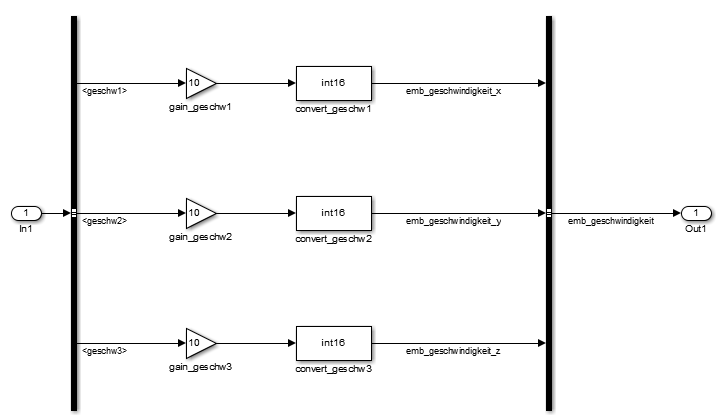
\includegraphics[scale = 0.77]{sc_daten_geschwindigkeit}
\caption[Übersicht über das Subsystem "`daten\_geschwindigkeit"\ im Subsystem "`daten\_dynamisch"\ im Signalkollektor]{Übersicht über das Subsystem "`daten\_geschwindigkeit"\ im Subsystem "`daten\_dynamisch"\ im Signalkollektor}
\label{scdatengeschwindigkeit}
\end{figure}

\newpage


Die weiteren Subsysteme im Subsystem \textit{"`daten\_dynamisch"} -- \textit{"`daten\_beschleunigung"}, \textit{"`daten\_gierrate"}, \textit{"`daten\_drehzahl\_rad"}, \textit{"`daten\_wassertemperatur"}, "`daten\_federweg"\ und \textit{"daten\_gaspedalstellung"} -- verhalten sich dazu äquivalent. Zu bemerken ist nur, dass der Multiplikator bei den Signalen des Subsystems \textit{"`daten\_gaspedalstellung"} nicht 10 sondern 1000 beträgt. \\

%-------------------------------------------------------------------%

\textit{Subsystem "`daten\_fahrdynamik" / Fahrdynamikregelung} \\

Wie in Abb. \ref{scdatenfahrdynamik} zu erkennen besteht das Subsystem genau wie das dazugehörige Subsystem im Signalgenerator nur aus zwei Signalen. Beide Werte werden wie üblich aus dem Busarray mittels eines Bus Selectors heraus getrennt. Beiden Signalen wird ein Multiplikator von 1000 durch die Gain-Blöcke zugeführt und die Konvertierung in \textit{int16} und Umbenennung findet durch die Convert-Blöcke statt. Darauf folgend werden beide Signale wieder mit einem Bus Creator gebündelt und das zusammengefasste Busarray wird mit dem Namen "`emb\_daten\_fahrdynamik"\ an das übergeordnete Subsystem \textit{"`Signalcollector\_Embedded\_PC"} übergeben. Die Weiterverarbeitung in diesem Subsystem gleicht der aus den vorherigen Kapiteln.

\begin{figure}[h]
\centering
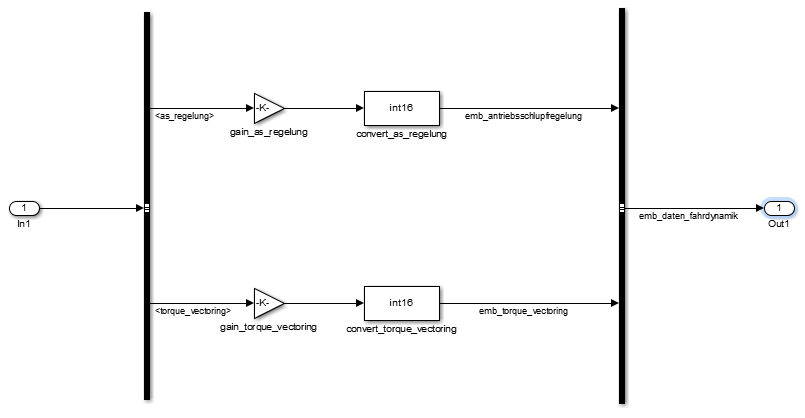
\includegraphics[scale = 0.75]{sc_daten_fahrdynamik}
\caption[Übersicht über das Subsystem "`daten\_fahrdynamik"\ im Signalkollektor]{Übersicht über das Subsystem "`daten\_fahrdynamik"\ im Signalkollektor}
\label{scdatenfahrdynamik}
\end{figure}

%-------------------------------------------------------------------%

\textit {Subsystem "`daten\_motor" / Motor- und Umrichterdaten}

Dieses Subsystem besitzt keinerlei besondere Eigenschaften, welche nicht bereits in den oberen Subsystemen beschrieben worden wären. Es besteht aus einem Subsystem und verschiedenen einzelnen Signalen (s. Abb. \ref{scdatenmotor}). Es sind keine boolean-Werte im Subsystem vorhanden. Die Aufbereitung der einzelnen Signale im Subsystem ist wie bei den Signalen in den vorherigen Kapiteln. Die Signale "`dc\_strom", "`dc\_spannung", "`lüfterdrehzahl"\ sowie "`mwassertemperatur" werden mittels Bus Selector aus dem Busarray separiert, erhalten einen Multiplikator von 10 durch die Gain-Blöcke und werden mittels der Convert-Blöcke in den Datentyp \textit{int16} konvertiert und umbenannt.

\newpage

Anschließend fasst sie der Bus Creator mit den anderen Signalen des Subsystems zusammen und übergibt die Daten an das Subsystem \textit{"`emb\_daten\_fahrdynamik"}. Die weitere Signalverarbeitung gleicht der aus den vorherigen Kapiteln in diesem Subsystem. Die Signale "`stromgrenze", "`maximalleistung", "`lüfter"\ und "`pumpe" werden analog behandelt, jedoch werden sie mit den Gain-Blöcken mit einem Multiplikator von 1000 versehen. Die Aufbereitung der Signale im Subsystem \textit{"`daten\_temperatur\_motor" }ist analog der des Subsystems \textit{"`daten\_geschwindigkeit"} zu betrachten.
 
\begin{figure}[h]
\centering
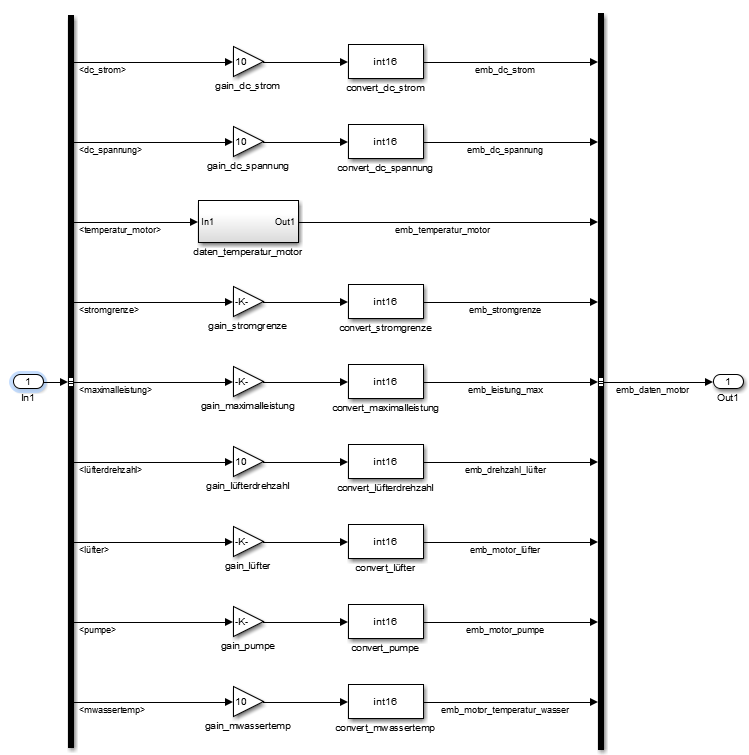
\includegraphics[scale = 0.75]{sc_daten_motor}
\caption[Übersicht über das Subsystem "`daten\_motor"\ im Signalkollektor]{Übersicht über das Subsystem "`daten\_motor"\ im Signalkollektor}
\label{scdatenmotor}
\end{figure} 

\newpage

%-------------------------------------------------------------------%
%-------------------------------------------------------------------%


\subsection{Signaltransmitter}
 
Der Signaltransmitter ist als letztes der drei übergeordneten Subsysteme des Simulink-Modells für die folgenden Aufgaben zuständig:

\begin{itemize}

\item Versand der im Signalkollektor (s. 2.1.4) aufbereiteten Fahrzeugdaten via Ethernet-Schnittstelle (UDP) an den Embedded-PC

\item Generierung der benötigten Informationen über das zu versendende Datenpaket

\item Versand dieser Paketinformationen an den Embedded-PC

\item Umsetzung der bidirektionalen Kommunikation zwischen der MicroAutoBox II und dem Embedded-PC

\end{itemize}

Im Folgenden soll daher nun anhand des Aufbaus des Signaltrannsmitters in Abb. \ref{subsignaltransmitter} die Realisierung der einzelnen Aufgabenbereiche innerhalb dieses Subsystems aufgezeigt werden. \\


%-------------------------------------------------------------------%


\textit{1) Versand der Fahrzeugdaten via Ethernet-Schnittstelle an den Embedded-PC} \\

Für diese Aufgabe sind die beiden Subsysteme \textit{"`MSGSIZE\_DATEN"} und \textit{"`UDP\_DATEN"} vorgesehen. Die Fahrzeugdaten, welche über den Inport-Block in das Subsystem geleitet werden, werden an den Port "`Data"\ des Subsystems "`UDP\_DATEN"\ gesendet, woraufhin sie via Ethernet-Schnittstelle an den Embedded-PC übertragen werden. Das Subsystem selbst besitzt den folgenden Aufbau:

\begin{figure}[h]
\centering
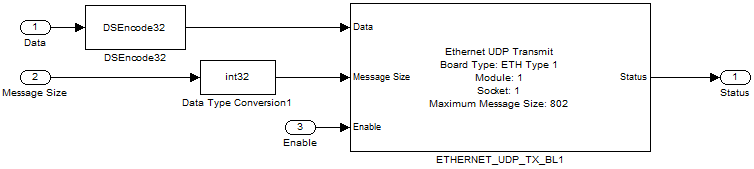
\includegraphics[scale = 0.75]{subudpdaten}
\caption[Übersicht über das Subsystem "`UDP\_DATEN"\ im Signaltransmitter]{Übersicht über das Subsystem "`UDP\_DATEN"\ im Signaltransmitter}
\label{scdatenmotor}
\end{figure} 

Wie aus den Erläuterungen im Entwurfsdokument bekannt ist (s. S.12-13), werden die Daten von einer sFunction \textit{DSEncode32} vom obligatorischen Datentyp \textit{double} am Eingang des Blockes in den Datentyp \textit{int16} gewandelt und als \textit{uint32} - Datenstrom an den Embedded-PC übertragen. An dem zweiten Port namens "`Message Size"\ des UDP-Send-Blockes (s. Entwurfsdokument S.13) soll ein konstanter Wert -- wie schon der Convert-Block andeutet -- im Datentyp \textit{int32} vorliegen, welcher die Paketgröße der zu versendenden Daten angibt. Um für die Fahrzeugdaten auch nach Änderungen des Simulink-Modells durch Hinzufügen oder Reduzieren von Fahrzeugdaten (s. 2.1.3) jeweils automatisch die korrekte Paketgröße zu ermitteln und an den Port "`Message Size"\ anzulegen, wurde das Subsystem \textit{MSGSIZE\_DATEN} dem Modell hinzugefügt (s. Abb. \ref{submsgsizedaten}). 

\newpage

\begin{figure}[h]
\centering
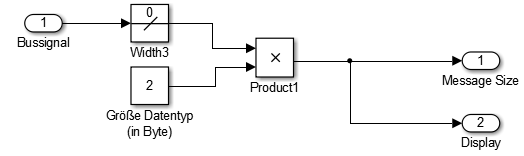
\includegraphics[scale = 0.75]{submsgsizedaten}
\caption[Übersicht über das Subsystem "`MSGSIZE\_DATEN"\ im Signaltransmitter]{Übersicht über das Subsystem "`MSGSIZE\_DATEN"\ im Signaltransmitter}
\label{submsgsizedaten}
\end{figure} 

In diesem Subsytem wird als Eingangssignal das Busarray der Fahrzeugdaten über einen Width-Block (s. S.5) geleitet und daraus die Breite des Busarrays bestimmt. Dieser Wert wird zusammen mit einem Constant-Block, welcher den Wert 2 besitzt, auf einen Product-Block geleitet und nach einer Konvertierung in den Datentyp \textit{int32} im Subsystem \textit{UDP\_DATEN} an den Port "`Message Size"\ angelegt. \\

Weiterhin muss im UDP-Send-Block nochmals die automatisch durch das Modell ermittelte Größe des Datenpaketes eingegeben werden, wofür leider noch nicht ein automatisierter Ablauf gefunden werden konnte. Dies dürfte allerdings spätestens in der Testphase behoben sein. \\


%-------------------------------------------------------------------%

\textit{2) Generierung der benötigten Informationen über das zu versendende Datenpaket} \\

\begin{figure}[h]
\centering
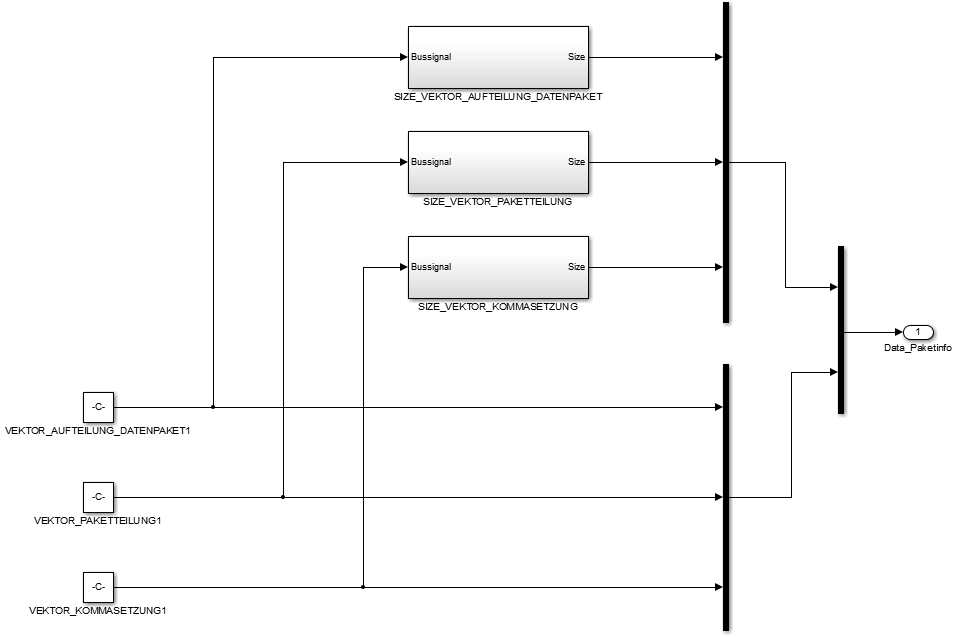
\includegraphics[scale = 0.6]{subdatenpaketinfo}
\caption[Übersicht über das Subsystem "`DATEN\_PAKETINFO"\ im Signaltransmitter]{Übersicht über das Subsystem "`DATEN\_PAKETINFO"\ im Signaltransmitter}
\label{subdatenpaketinfo}
\end{figure} 

\newpage

Diese Aufgabe wird ausschließlich durch das Subsystem \textit{DATEN\_PAKETINFO} bewerkstelligt. Hierbei werden in drei Constant-Blöcke die zuvor in der Config-Datei config\_datenpaket.m referenzierten Vektoren (s. 2.1.2) eingebunden und von ebendiesen durch drei Subsysteme deren jeweilige Breiten ausgelesen. Diese Signalvektoren und die jeweilige Größen der Vektoren werden getrennt auf einen Multiplexer geleitet und abschließend nochmals mittels eines Multiplexers zu einem Gesamtsignalvektor "`data\_paketinfo"\ zusammengefasst, welcher nach dem Verlassen des Subsystem die folgende Struktur aufweist: \\

$ data\_paketinfo = \left( \begin{array}{c} SIZE\_VEKTOR\_AUFTEILUNG\_DATENPAKET \\ SIZE\_VEKTOR\_PAKETTEILUNG \\ SIZE\_VEKTOR\_KOMMASETZUNG \\ VEKTOR\_AUFTEILUNG\_DATENPAKET \\ VEKTOR\_PAKETTEILUNG \\ VEKTOR\_KOMMASETZUNG  \end{array} \right)$ 

\vspace*{5mm}

%-------------------------------------------------------------------%

\textit{3) Versand der Paketinformationen an den Embedded-PC} \\

Der Versand der Paketinformationen an den Embedded-PC erfolgt im Subsystem \\ "`UDP\_PAKETINFORMATIONEN"\ auf analoge Weise zu dem Versand der Fahrzeugdaten (statt des Subsystems "`MSGSIZE\_DATEN" wird hier nur das dazu inhaltlich äquivalente Subsystem "`MSGSIZE\_PAKETINFO"\ verwendet). Lediglich bei der Konvertierung wird aufgrund der begrenzten maximalen Paketgröße eines Paketes beim UDP-Protokoll von  1472 byte der Datentyp \textit{unit8} ausgewählt, um den Versand aller Paketinformationen in einem einzigen Paket zu ermöglichen. Demzufolge muss auch im Subsystem \\ "`MSGSIZE\_PAKETINFO"\, welches die Paketgröße ermittelt, beim Constant-Block der Wert  "`2" beim Produktblock durch den Wert  "`1"\ ersetzt oder zusammen mit dem Produktblock entfernt werden. \\



%-------------------------------------------------------------------%

\textit{4) Umsetzung der bidirektionalen Kommunikation zwischen der MicroAutoBox II und dem Embedded-PC} \\

Die Umsetzung der bidirektionalen Kommunikation zwischen der MicroAutoBox II und dem Embedded-PC wird durch das Subsystem "`EMB\_RECEIVE"\ (s. Abb. \ref{subembreceive})  und zwei UND-Gattern (s. S.4) realisiert. Ein UDP-Receive-Block -- das Gegenstück zum UDP-Send-Block -- empfängt von dem Embedded-PC einen Bytevektor, welcher mittels der sFunction \textit{DSDecode32} dekodiert wird. Nachdem dieser anschließend über einen Demultiplexer geleitet wurde, werden die verschiedenen Sample Times des Demultiplexers und der sFunction "`Byte\_to\_8Bit\_Decoder"\ mittels eines Rate-Transition-Blocks (s. S.5) aneinander angeglichen. Letzterer Block sorgt dafür, dass aus dem gesendeten Bytevektor die einzelnen Bits getrennt herausgeführt werden können. Von diesen 8 Bits werden jedoch nur 4 Bits (Bit 0-3) benötigt, wodurch die anderen 4 Bits frei gewählt werden können. Die Bits 0-3 werden nun nach einer Konvertierung in den Datentyp \textit{boolean} an zwei RS-Flip-Flops (s. S.7) angeschlossen, welche nach einem weiteren Rate-Transition-Block aus dem Subsystem herausgeführt werden. Anschließend werden die Signale an zwei UND-Gatter auf der in Abb. \ref{subsignaltransmitter} gezeigten Weise angeschlossen, deren Ausgänge jeweils mit dem Input "`Enable"\ der beiden Subsysteme "`UDP\_DATEN"\ und "`UDP\_PAKETINFORMATIONEN"\ verbunden sind. Somit lässt sich je nach dem Inhalt des an die MicroAutoBox II übertragenen Bytevektors vom Embedded-PC aus genau steuern, welcher von den beiden UDP-Send-Blöcken -- "`UDP\_DATEN"\ oder "`UDP\_PAKETINFORMATIONEN"\ -- aktiv sein sollen, was durch die nachfolgende Tabelle nochmals verdeutlicht werden soll:

\begin{table}[h]
\centering

\caption{Wertetabelle Bytevektor}

 \begin{tabular}{ c | c | c }
 
 \toprule[1.5pt]
 Bytevektor (LSB - MSB) & UDP\_DATEN   &  UDP\_PAKETINFORMATIONEN  \\
 \midrule
  $[1 0 1 0 * * * *]$ & 0 & 0     \\
\midrule  
  $[0 1 1 0 * * * *]$ & 0 & 1     \\
\midrule  
  $[1 0 0 1 * * * *]$ & 1 & 0     \\

 
 \bottomrule[1.5pt] 
 
\end{tabular}

\end{table}

\newpage

%-------------------------------------------------------------------%
    

   


 









  
 



   

%--------------------------  Embedded PC  --------------------------%

\section{Embedded PC und virtueller Server}

An der Datenübertragung und Verarbeitung sind drei von uns entworfene Anwendungen beteiligt. Aus dem in Abschnitt 2.1 (VERWEIS) bereits beschriebenen Simulink-Modell wird mithilfe der Entwicklungswerkzeuge von dSPACE automatisch C-Code erzeugt und für die Ausführung auf der MicroAutoBox II kompiliert. Diese Anwendung wird im Folgenden als \textit{mabxii} bezeichnet. Desweiteren wird jeweils eine von uns in C++ implementierte Anwendung auf dem Embedded-PC und vServer laufen welche von nun an \textit{embpc} und \textit{vserver} genannt werden. Bei deren Entwurf wurde insbesondere darauf geachtet, dass beiden Anwendungen eine möglichst große gemeinsame Code-Basis zugrundeliegt. Dadurch soll zum einen die Fehlerwahrscheinlichkeit minimiert werden -- Code-Abschnitte werden häufiger ausgeführt wodurch Fehler eher zutage treten und behoben werden können -- und zum anderen soll dadurch Zeit bei der Implementierung und dem Testen eingespart werden die letztendlich der Qualität der Software zugute kommt. 

Im Folgenden wird die konkrete Funktionsweise dieser drei Anwendungen anhand einer schrittweisen Beschreibung eines Kommunikationsverlaufs erläutert. Siehe dazu auch Abbildung (VERWEIS).

\subsection{Initialisierung}

\begin{itemize}

\begin{figure}[H]
\centering
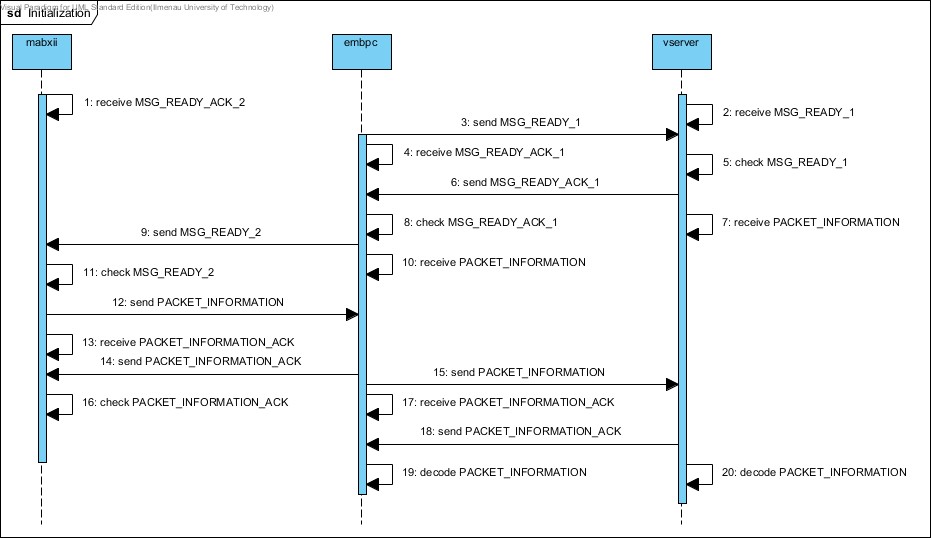
\includegraphics[scale = 0.75]{Initialization}
\caption[Initialisierung der Kommunikation]{Initialisierung der Kommunikation}
\label{inite}
\end{figure}

\item[1) - 2)] 
Der virtuelle Server sowie die MicroAutoBox sind nach deren Start in einer Art Wartezustand(\texttt{1/2: receive MSG\_READY}) in dem sie auf die Nachricht \texttt{MSG\_READY} des Embedded-PCs warten. Dabei handelt es sich um einen mit einer bestimmten Bitfolge bestückten Bitvektor der Länge 1 Byte. (Siehe Abbildung VERWEIS) Dieser signalisiert beiden Teilnehmern die Bereitschaft des Embedded-PCs. 

\item [3) - 4)]
Sobald der Embedded-PC hochgefahren ist wird die Anwendung \emph{embpc} automatisch ausgeführt. Der PC ist nach fehlerfreiem Start dazu in der Lage sein erstes Paket zu senden und damit seine Bereitschaft mitzuteilen. Das Paket \texttt{MSG\_READY} wird über eine UMTS-Verbindung zunächst an den virtuellen Server gesendet (\texttt{3: send MSG\_READY})und beinhaltet den oben beschriebenen Bitvektor. Nach dem Sendevorgang wartet er auf ein Acknowledgement \texttt{MSG\_READY\_ACK} des vServers (\texttt{4: receive MSG\_READY\_ACK}).


\item[5) - 7)]
Hat der virtuelle Server diesen Bitvektor erfolgreich empfangen wird dieser zunächst dekodiert und auf seine Richtig- bzw. Vollständigkeit geprüft (\texttt{5: check MSG\_READY}). Danach sendet dieser dem Embedded-PC eine Empfangsbestätigung (\texttt{6: send MSG\_READY\_ACK}), wieder in Form eines 8 bit großen Bitvektors bestimmter Kodierung (siehe Abbildung VERWEIS). Anschließend wartet der vServer auf ein Paket \texttt{PACKET\_INFO} (\texttt{7: receive PACKET\_INFO}. Wurde nicht der erwartete Bitvektor empfangen wird wieder mit Schritt \texttt{2: receive MSG\_READY} fortgefahren.

\item[8) - 10)]
Sobald das Paket \texttt{MSG\_READY\_ACK} den Embedded-PC erreicht wird dies wie auf dem vServer zunächst dekodiert und überprüft (\texttt{8: check MSG\_READY\_ACK}). Falls es korrekt empfangen wurde meldet die Anwendung \emph{embpc} nun ihre Bereitschaft an die MicroAutoBox II durch das Senden der Nachricht \texttt{MSG\_READY} (\texttt{9: send MSG\_READY}) und wartet anschließend auf ein Paket (\texttt{10: receive PACKET\_INFO}. Falls jedoch nach 5 Sekunden noch kein Acknowledgement des vServers eingetroffen ist, wird wieder mit Schritt \texttt{3: send MSG\_READY} begonnen.

\item[11)- 13)]
Hier wird auf der MicroAutoBox II analog zu schritt 5 und 8 verfahren und das ankommende Paket zunächst überprüft (\texttt{11: check MSG\_READY}). Wurde nicht das erwartete Paket empfangen wird mit Schritt 1 fortgefahren. Ansonsten sendet die MicroAutoBox II ein Paket das die Informationen zur Paketaufteilung, der Kommaverschiebung  und Datentypen der einzelnen Werte beinhaltet an den Embedded PC (\texttt{12: send PACKET\_INFO}). Danach wird auf eine Empfangsbestätigung des Embedded-PC gewartet (\texttt{13: receive PACKET\_INFO\_ACK}). Trifft diese nicht innerhalb von 5 Sekunden ein, wird die Nachricht erneut verschickt. 

\item[14) - 17)]
Nachdem der Embedded-PC das Paket \texttt{PACKET\_INFO} empfangen hat schickt er zunächst eine Empfangsbestätigung an die MicroAutoBox II (\texttt{14: send PACKET\_INFO\_ACK}) und leitet anschließend das Paket an den vServer weiter (\texttt{15: send PACKET\_INFO}). Nun wartet er auf die Empfangsbestätigung des vServers (\texttt{17: receive PACKET\_INFO\_ACK}). Falls innerhalb von 5 Sekunden keine Nachricht eintrifft wird das Paket erneut verschickt.

\item[18) - 20)]
Sobald der vServer das Paket \texttt{PACKET\_INFO} entgegen nimmt bestätigt er dessen Empfang (\texttt{18: send PACKET\_INFO\_ACK}) und fängt anschließend mit der Dekodierung der Paketinformationen an (\texttt{20: decode PACKET\_INFORMATION}). Dabei werden die einzelnen Daten (Paketaufteilung, Kommaverschiebung und Datentypen) in einer jeweils eigenen Datenstruktur abgelegt (\texttt{VEC\_LAYOUT, VEC\_COMMA, VEC\_DATATYPES}). Auf diese wird im späteren Verlauf zugegriffen um die Fahrzeugdaten korrekt verarbeiten zu können. Der Embedded-PC verfährt nach dem Empfang der Empfangsbestätigung genauso (\texttt{19: decode PACKET\_INFO}).

\end{itemize}

Der Grund für diesen ausführlichen Initialisierungsprozess ist, dass es für die Verarbeitung der Fahrzeugdaten wichtig ist, dass sowohl der Embedded-PC als auch der vServer über die Paketinformationen verfügen. Durch deren Größe wäre es aufgrund der geringen Bandbreite von UMTS/GPRS keine Option diese mit jedem Datenpaket zu übertragen. Falls sich die bisherige Initialisierung in der Testphase als zu fehleranfällig herausstellen sollte, indem z.B. keine Datenübertragung zustande kommt weil zu viel Paketverlust auftritt, wird dieser Prozess selbstverständlich überarbeitet. Das bisherige Konzept ist also noch nicht endgültig.

\subsection{Datenübertragung und Datenverarbeitung}

\begin{itemize}

\begin{figure}[H]
\centering
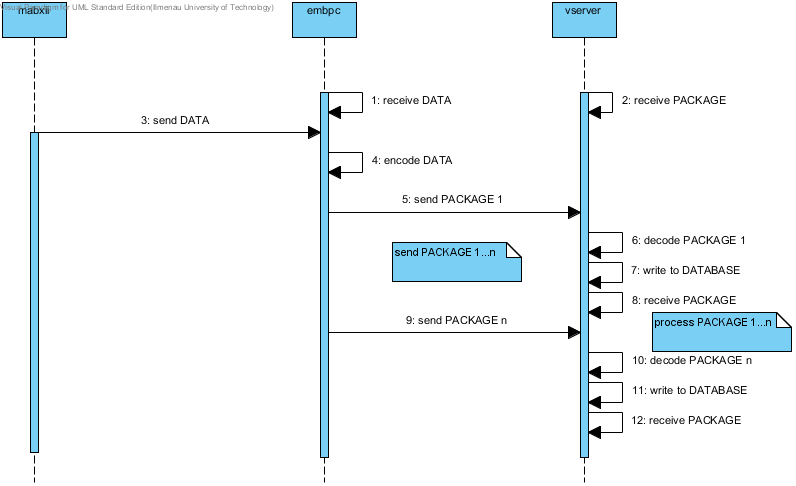
\includegraphics[scale = 0.75]{Data_Transmission}
\caption[Übertragung der Fahrzeugdaten]{Übertragung der Fahrzeugdaten}
\label{datatrans}
\end{figure}

\item[1) - 3)]
Nachdem die MicroAutoBox die Empfangsbestätigung des \texttt{PACKET\_INFO} vom Embedded-PC erhalten hat beginnt sie nun in einem festen Zeitabstand UDP-Pakete mit aktuellen Fahrzeugdaten an den Embedded-PC zu senden (\texttt{3: send DATA}). Dabei wird nicht berücksichtigt ob die Pakete den Embedded-PC auch tatsächlich erreichen. Die Konfiguration des Zeitabstandes erfolgt im Matlab/Simulink-Programm mit Hilfe einer sogenannten sample-time (optional-clock). Sowoh der Embedded-PC als auch der vServer warten nun auf ankommende Daten (\texttt{1: receive DATA, 2: receive PACKAGE}).

\item[4) - 12)]
Der Embedded-PC nimmt die Fahrzeugdaten entgegen und verarbeitet diese (\texttt{4: encode DATA}). Dabei wird der Datensatz \texttt{DATA} entsprechend der Informationen in \texttt{VEC\_LAYOUT} in mehrere Pakete geteilt und mit einem \texttt{HEADER} versehen. Anschließend werden diese Pakete der Reihe nach an den vServer übertragen (\texttt{5,9,...: send PACKAGE 1,...,n}). Dabei wird keine Empfangsbestätigung am Server erzeugt und somit auch keine am Embedded-PC erwartet. 
Nach Abschluss der Entwurfsphase wurde die Idee umgesetzt die eingehenden Fahrzeugdaten am Embedded-PC in mehrere Pakete aufzuteilen, um bei eventuell auftretenden Verbindungsproblemen zumindest einzelne Pakete erfolgreich an den virtuellen Server übertragen zu können. Das Programm auf dem PC sorgt dafür, dass jedes Paket vor dem Senden mit einem aktuellen 8 Byte Zeitstempel und einer 4 Byte Identifikationsnummer (ID) versehen ist (Zeitstempel + ID = \texttt{HEADER}). Zum Erzeugen des Zeitstempels, mit Nanosekunden-Auflösung wird die Echtzeituhr des PCs genutzt (clock\_gettime(CLOCK\_REALTIME, Zeitstempel-Variable)). Die ID repräsentiert die Paketnummer, ist also eine Zahl zwischen 1 und der Anzahl der getrennten Pakete. Standardmäßig wurde diese in Anlehnung an das Pflichtenheft auf fünf Pakete gesetzt, kann aber im mabxii Programm geändert werden. \\
Sobald ein Paket den vServer erreicht wird es zunächst dekodiert (\texttt{6: decode PACKAGE 1}) (wobei \texttt{PACKAGE 1} hier nicht zwangsläufig das erste Paket aus \texttt{DATA} sein muss - Pakete können sich überholen oder verloren gehen). Dabei wird zunächst der \texttt{HEADER} ausgelesen. Der darin enthaltene Zeitstempel wird mit dem lokalen verglichen, ist die Differenz größer als 5 Sekunden wird das Paket verworfen, ansonsten wird das Paket entsprechend der Daten in \texttt{VEC\_LAYOUT}, \texttt{VEC\_COMMA} und 7\texttt{VEC\_DATATYPES} so bearbeitet, dass der Dekoder einen Fahrzeugwert nach dem anderen an die Datenbank zur Verfügung stellen kann. Wurden alle Fahrzeugdaten aus dem Paket ausgelesen und verarbeitet, wird ein neues Paket empfangen. 

\end{itemize}

Tritt ein Neustart des Embedded-PCs mitten im Kommunikationsvorgang auf, führt das erneute Senden des Pakets \texttt{MSG\_READY} an den virtuellen Server zu dessen Reaktion den aktuellen Kommunikationsvorgang abzubrechen und sich auf einen neuen vorzubereiten -- der Initialsierungsprozess beginnt von neuem. Auch das Senden des Pakets \texttt{MSG\_READY} an die MicroAutoBox II dient dazu einen neuen Kommunikationsvorgang mitzuteilen, denn durch dessen Empfang bricht auch diese den aktuell laufenden Kommunikationsvorgang ab und beginnt einen neuen Vorgang. Ein weiterer kritischer Punkt ist das nicht Empfangen der Fahrzeugdaten des Servers, wird das Programm nach einem von uns festgelegten Zeitpunkt (timeout X) keine Pakete empfangen, reagiert es durch ein erneutes Senden des Paketes (ready\_2) an den Embedded-PC. Daraufhin sendet der PC nach Empfang des Paketes erneut das Paket (ready\_3), was einen neuen Kommunikationsvorgang auslöst. 

\begin{table}[H]
\centering

\caption{Übersicht über die Inhalte der übertragenen Pakete}

 \begin{tabular}{ c | p{4cm} | p{1.5cm} | p{2cm} | p{4cm} }
 
 \toprule[1.5pt]
 
 Paket\-bezeichnung & Inhalt & Sender & Empfänger & Bemerkung \\
 
 \midrule
 
MSG\_READY\_1 & Bitvektor: \texttt{[01011001]} & \emph{embpc} & \emph{vserver} &

\vspace*{-8mm}

\begin{itemize}[leftmargin=*] 

\item Kommunikations\-beginn melden
\item ggf. Mitteilung über neuen Kommunikationsbeginn

\end{itemize} \\

\midrule

MSG\_READY\_ACK\_1 & Bitvektor: \texttt{[01010001]} & \emph{vserver} & \emph{embpc} & Empfangsbestätigung für MSG\_READY\_1 \\

\midrule

MSG\_READY\_2 & Bitvektor: \texttt{[10010101]} & \emph{embpc} & \emph{mabxii} &

\vspace*{-8mm}

\begin{itemize}[leftmargin=*]
\item Bereitschaft von vServer und Emb-PC melden
\item ggf. Mitteilung über neuen Kommunikationsbeginn
\end{itemize} \\

\midrule

PACKET\_INFO & Bytestrom: ([VEC\_DATATYPES], [VEC\_LAYOUT], [VEC\_COMMA]) &
\emph{mabxii} \emph{embpc}& \emph{embpc} \emph{vserver} & 

\vspace*{-8mm}

\begin{flushleft}
Beinhaltet die für den Emb-PC und vServer notwendigen Informationen für die nachfolgende Verarbeitung der Fahrzeugdaten
\end{flushleft} \\

\midrule

PACKET\_INFO\_ACK\_1 & Bitvektor: \texttt{[00010101]} & \emph{embpc} & \emph{mabxii} & 
Empfangsbe\-stätigung für PACKET\_INFO \\

\bottomrule[1.5pt] 
 
\end{tabular}

\end{table}

\newpage

\begin{table}[H]
\centering

\caption{Übersicht über die Inhalte der übertragenen Pakete - Fortsetzung}

\begin{tabular}{c | p{4cm} | p{1.5cm} | p{2cm} | p{4cm} }
 
\toprule[1.5pt]

Paket\-bezeichnung & Inhalt & Sender & Empfänger & Bemerkung \\
 
\midrule

PACKET\_INFO\_ACK\_2 & Bitvektor: \texttt{[01000101]}

& \emph{embpc} & \emph{vserver} & Empfangsbestäti\-gung für PACKET\_INFO
 \\

\midrule

DATA & 

\vspace*{-8mm}

\begin{itemize}[leftmargin=*]

\item Beinhaltet sämtliche und aktualisierte Fahrzeuginformationen

\item Der Inhalt wird immer aktuell gehalten

\end{itemize} 

& \emph{mabxii} & \emph{embpc} & Wird ohne Abfrage des Empfangs kontinuierlich gesendet \\

\midrule

PACKAGE & 

\vspace*{-8mm}

\begin{itemize}[leftmargin=*]

\item von \emph{embpc} in Pakete aufgeteilte aktuelle Fahrzeuginformationen, versehen mit jeweiligen Zeitstempel und ID

\item ([TIMESTAMP], [ID], [DATA\_N])

\end{itemize} 

& \emph{embpc} & \emph{vserver} & 

\vspace*{-8mm}

\begin{itemize}[leftmargin=*]

\item Standardmäßig werden die Fahrzeugdaten in 5 unterschiedliche Pakete aufgeteilt

\item Der sich ändernde Informationsinhalt der einzelnen Pakete wird durch den Datenempfang von der MABX II auf dem Emb-PC ständig aktualisiert.

\end{itemize} \\

\bottomrule[1.5pt]

\end{tabular}

\end{table}

\newpage

% Einfügen von Tobias' Sachen:


\subsection{Einfügen in die Datenbank}

\begin{figure}[h]
\centering
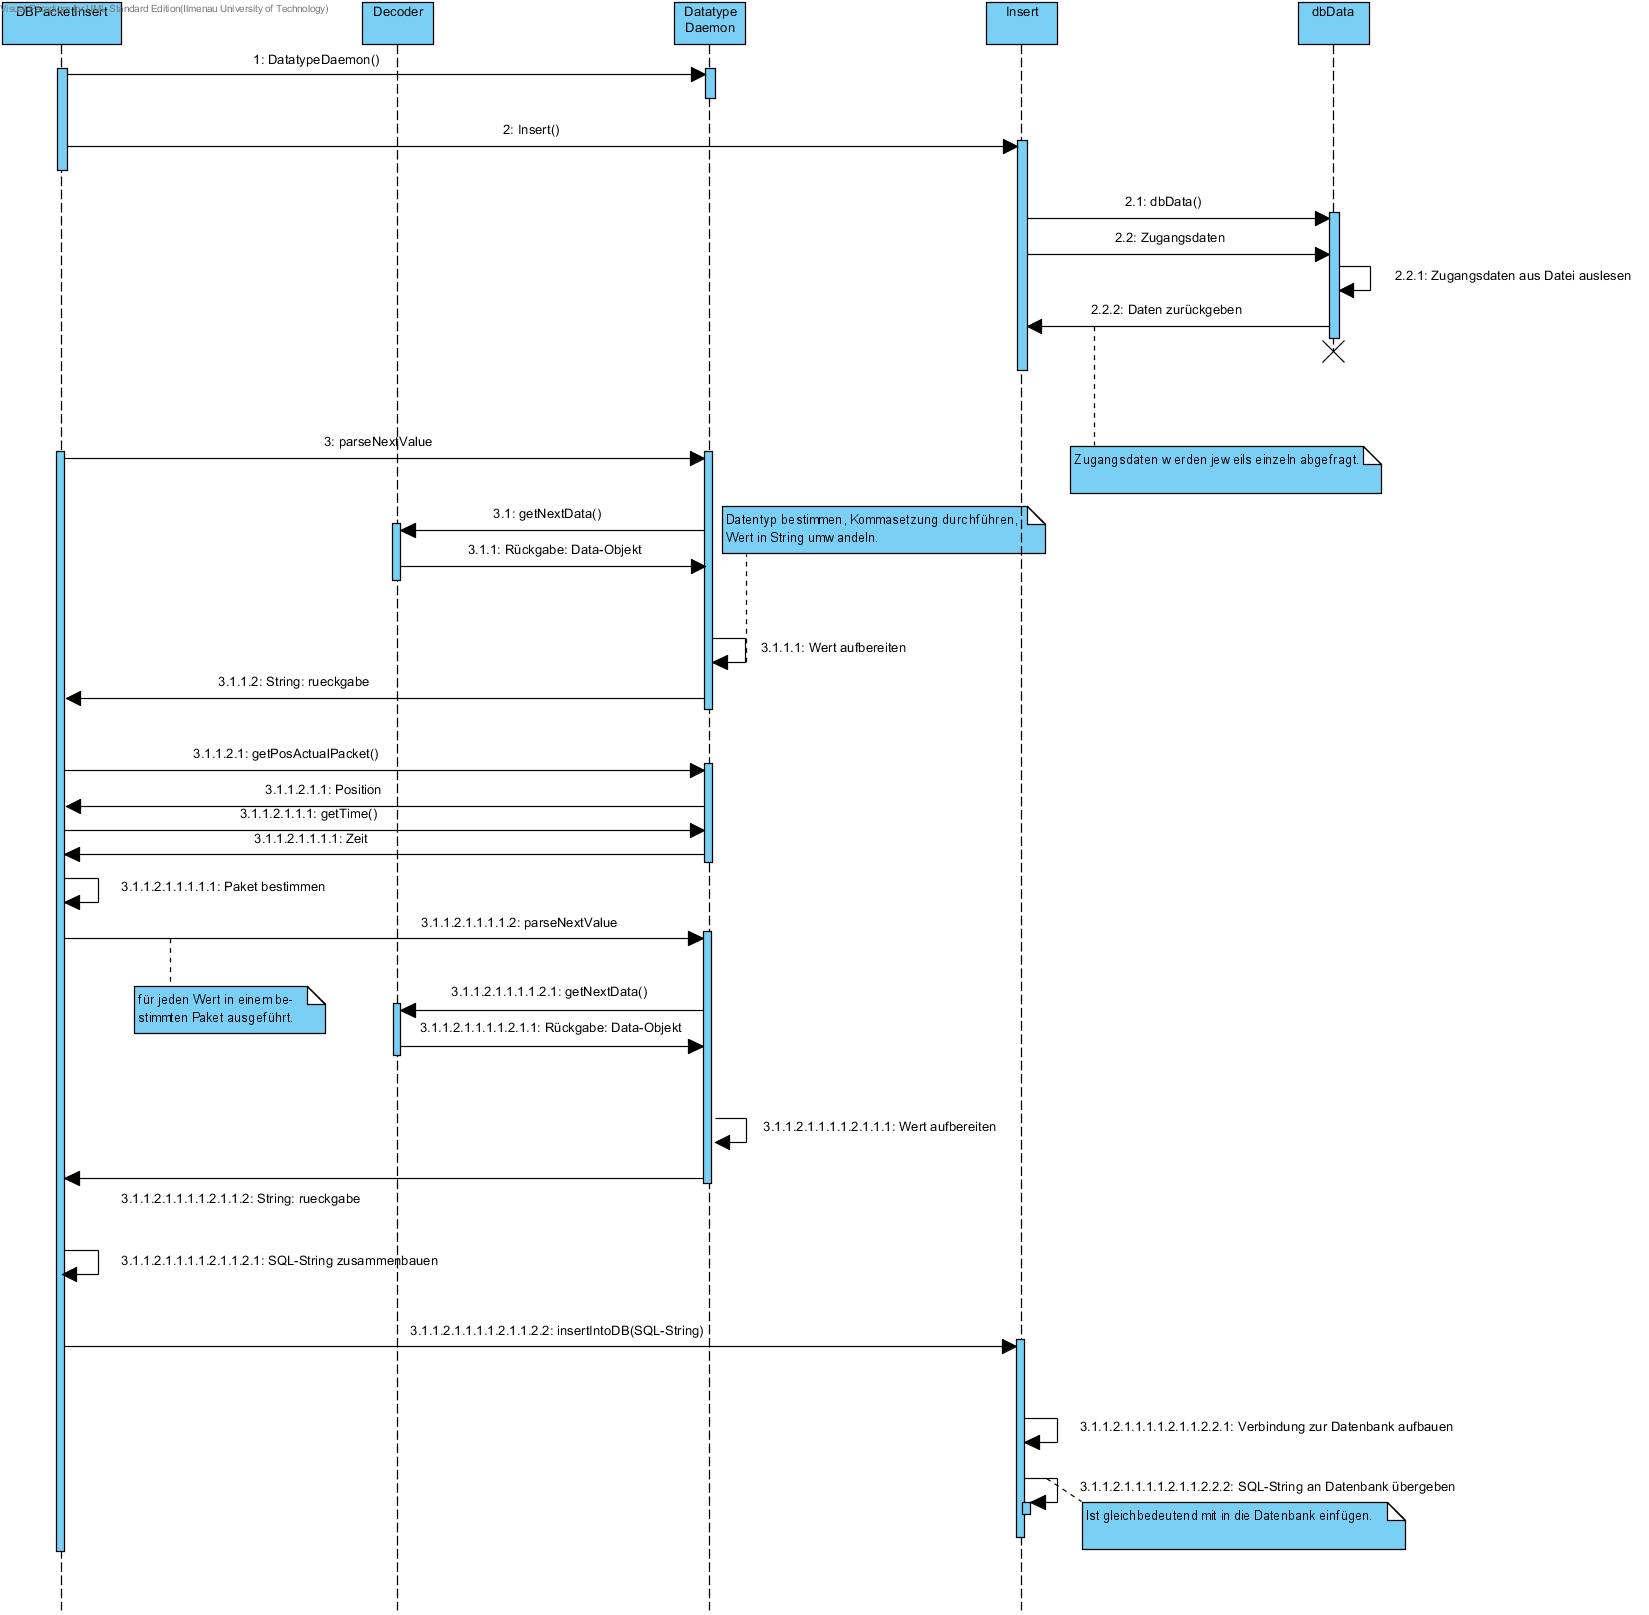
\includegraphics[scale = 0.5]{Datenbank_einfuegen}
\caption[Sequenzdiagramm zum Einfügen in die Datenbank]{Sequenzdiagramm zum Einfügen in die Datenbank}
\label{classvServer}
\end{figure}


%%%%%%%%%%%% HIER TEXT %%%%%%%%%%%%%%%%
Dieses Sequenzdiagramm zeigt den typischen Ablauf vom Start des Programms bis zum Ende einer Einfügeoperation in die Datenbank.\\
Es wird dabei davon ausgegangen, dass die Klasse Decoder bereits existiert.\\
Zuerst wird ein Objekt von \textit{DBPacketInsert} erzeugt, das wiederum zuerst jeweils ein Objekt der Klasse \textit{DatatypeDaemon} und \textit{Insert} erzeugt. \textit{Insert} erzeugt daraufhin ein Objekt der Klasse \textit{dbData}, welches ihm die Zugangsdaten zur Datenbank zurückgibt. Das Objekt \textit{dbData} wird daraufhin gelöscht. Danach wird bei \textit{DBPacketInsert} die Memberfunktion \textit{db\_insert()} aufgerufen. Leider war zu diesem Zeitpunkt wie in der Einleitung noch nicht klar, von wem diese Funktion aufgerufen wird, daher findet sie sich hier nicht wieder. Sie löst aber Schritt drei im Diagramm aus, wodurch ein einzelner Wert durch \textit{DatatypeDaemon} geholt wird, den dieser wiederum eingebettet in ein Data-Objekt vom \textit{Decoder} bekommt. Dieser Wert ist immer der Anfang eines Übertragungspakets von Embedded PC zum vServer. Zunächst wird das Paket durch die Position des einzelnen Wertes bestimmt, danach wird \textit{DatatypeDaemon} so oft nach neuen Werten angefragt, bis ein Paket komplett abgehandelt ist. Danach wird der SQL-String aus diesen abgefragten Einzelwerten in einer Unterfunktion zusammengesetzt und anschließend an \textit{insertIntoDB(SQL-String)} des Objekts der Klasse \textit{Insert} übergeben. Dieses baut zuerst eine Verbindung zur Datenbank auf und übergibt dann den SQL-String der Datenbank bzw. dem MySQL-Connector/C++.

%%%%%%%%%%%%%%%%%%%%%%%%%%%%%%%%%%%%%%%

\newpage % brauchst du evtl. nochmal, mal sehen wies passt

\begin{figure}[h]
\centering
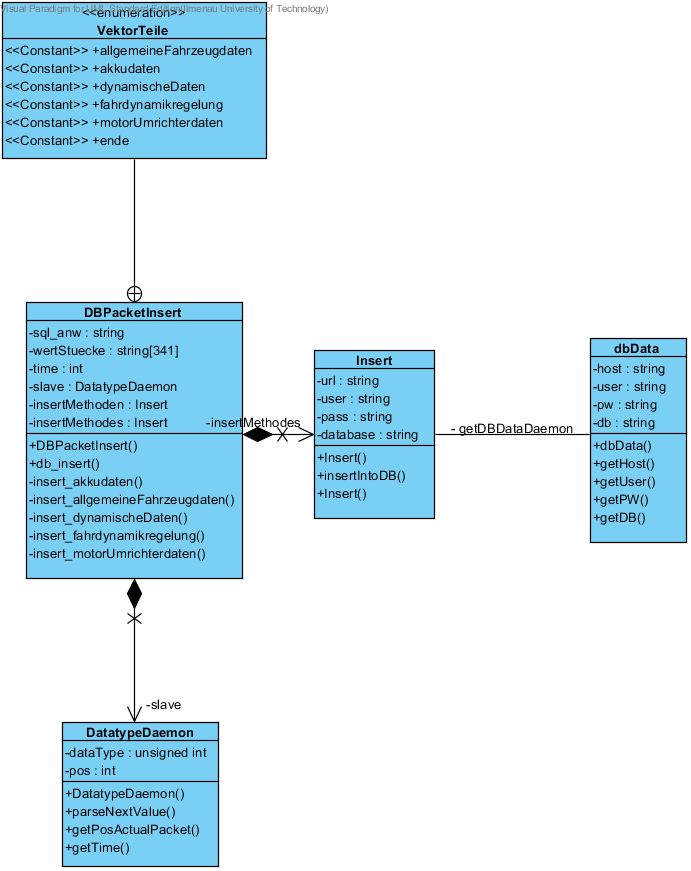
\includegraphics[scale = 0.9]{vServer}
\caption[Klassendiagramm des virtuellen Servers]{Klassendiagramm des virtuellen Servers}
\label{classvServer}
\end{figure} 

%%%%%%%%%%%% HIER TEXT %%%%%%%%%%%%%%%%
Klasse \textit{DBPacketInsert}:

Von dieser Klasse soll, wenn das Programm vollständig zusammengebaut ist, einmal ein Objekt erzeugt werden, auf dem dann jeweils nach Erhalt eines Paketes vom Embedded PC die Memberfunktion \textit{db\_insert()} aufgerufen wird. Diese löst dann das Auslesen und Aufbereiten der einzelnen Daten in der Klasse \textit{DatatypeDaemon} aus, setzt die Werte zusammen zu einem SQL-String und übergibt diesen an die Klasse \textit{Insert}. Im Weiteren wird auf diese einzelnen Schritte näher eingegangen.\\
Wie oben bereits geschildert, fragt \textit{DBPacketInsert} zuerst nur einen Wert von \textit{DatatypeDaemon} an und fügt diesen in ein Stringarray ein. Zu diesem Wert lässt es sich außerdem die Stelle im Übertragungspaket der MikroAutoboxII zum Embedded PC übergeben. Dies geschieht zum einen durch den Aufruf von \textit{parseNextValue()} auf \textit{DatatypeDaemon}, zum anderen durch den Aufruf von \textit{getPosActualPacket()} auf derselben Klasse. Danach fragt \textit{DBPacketInsert} über \textit{DatatypeDaemon} die Stelle des Wertes im Übertragungspaket von MikroAutoboxII zum Embedded PC ab, woraus er dann das Übertragungspaket von Embedded PC zum vServer ermittelt. Ein solches Paket beinhaltet alle Daten einer Tabelle auf der Datenbank, er nutzt dazu auch die in einer Enumeration definierten Startpunkte der einzelnen Pakete, die den Stellen im Übertragunspaket der MikroAutoboxII zum Embedded PC entsprechen. Diese Information benötigt die Klasse, um jetzt nur so viele Werte über \textit{DatatypeDaemon} in dem Array, welches schon den einen oben genannten Wert enthält, zu sammeln, wie in einem Übertragungspaket sind. Damit füllt der gesamte Inhalt des Arrays eine Tabelle der Datenbank aus.\\
Für jede Tabelle gibt es schließlich eine Unterfunktion, die entsprechend dem Aufbau der Datenbank die einzelnen Werte des Arrays zusammensetzt und daraus einen gültigen SQL-String baut. Sobald die Unterfunktion abgeschlossen ist, wird der fertige SQL-String an die Memberfunktion \textit{insertIntoDB(string* anw)} der Klasse \textit{Insert} übergeben.\\
\\
\\
Klasse \textit{DatatypeDaemon}:\\
Diese Klasse stellt die Schnittstelle zum Decoder dar, indem sie dort \textit{Data}-Objekte anfragt. Aus diesen Objekten extrahiert sie dann jeweils den Datenwert als \textit{Unsigned Integer}, die Position dieses Wertes in dem Übertragungspaket der MikroAutoBoxII an den Embedded PC, den Datentyp vor der Übertragung und den Kommasetzwert.\\
Einerseits stellt \textit{DatatypeDaemon} der Klasse \textit{DBPacketInsert} die Zeit als auch die Position des aktuellen Wertes bereit, andererseits stellt sie auch den Zeitstempel des Pakets, den die Klasse auch vom \textit{Decoder} erhält, zur Verfügung. Die Position ist dabei über die Memberfunktion \textit{getPosActualPacket()}, der Zeitstempel über \textit{getTime()} abzufragen.\\
Der Wert hingegen wird von der Klasse zuerst auf seinen Datentyp geprüft, dann gegebenenfalls durch die vom Kommasetzwert vorgegebene Zehnerpotenz geteilt und in den jeweiligen Datentyp verwandelt. Danach wird der Wert unter Verwendung der von der \textit{Boost-Library} angebotenen Funktion \textit{lexical\_cast} in einen \textit{String} konvertiert. Dies geschieht bei Aufruf der Memberfunktion \textit{parseNextValue()}, der aufbereitete und in einen \textit{String} verwandelte Wert bildet dabei den Rückgabewert an den Aufrufer.\\
\\
\\
Klasse \textit{Insert}:\\
Diese Klasse übernimmt die Kommunikation mit der Datenbank. Dazu erstellt sie erst ein Objekt der Klasse \textit{dbData}, das über die Memberfunktionen \textit{getHost()}, \textit{getUser()}, \textit{getPW()} und \textit{getDB()} jeweils die Adresse, den Benutzer, das Passwort und den Namen der Datenbank zurückgibt.\\
Wird von \textit{Insert} die Memberfunktion \textit{instertIntoDB(string* anw)} aufgerufen, so wird zunächst unter Zuhilfenahme des\textit{MySQL-Connector/C++} eine Verbindung mit der Datenbank aufgebaut und an den \textit{Connector} der \textit{String anw} übergeben, der zu diesem Zeitpunkt eine vollständige SQL-Anweisung darstellt. Durch die Übergabe des Strings erfolgt dann das Einfügen der Daten durch den \textit{Connector}.

%%%%%%%%%%%%%%%%%%%%%%%%%%%%%%%%%%%%%%%




%--------------------------   vServer   ----------------------------%

%\section{vServer}



%--------------------------   Webseite  ----------------------------%

\section{Webseite}

% % % % % % % % % % % % % %
%       FEINENTWURF       %
% % % % % % % % % % % % % %

\subsection{Aufbau der Webseite}
Die Webseite setzt sich aus einer Vielzahl von einzelnen PHP- und Java-Skripten zusammen, die gemeinsam die geforderte Funktionalität erfüllen. Um dem Leser einen einigermaßen geordneten Überblick über diese zu verschaffen, möge er das folgende Diagramm näher betrachten. Hier sind alle Skripte und ihre gegenseitigen Zusammenhänge zu finden und stellen den genauen Aufbau der kompletten Webseite dar.

% Komponentendiagramm %
\begin{figure}[h]
\centering
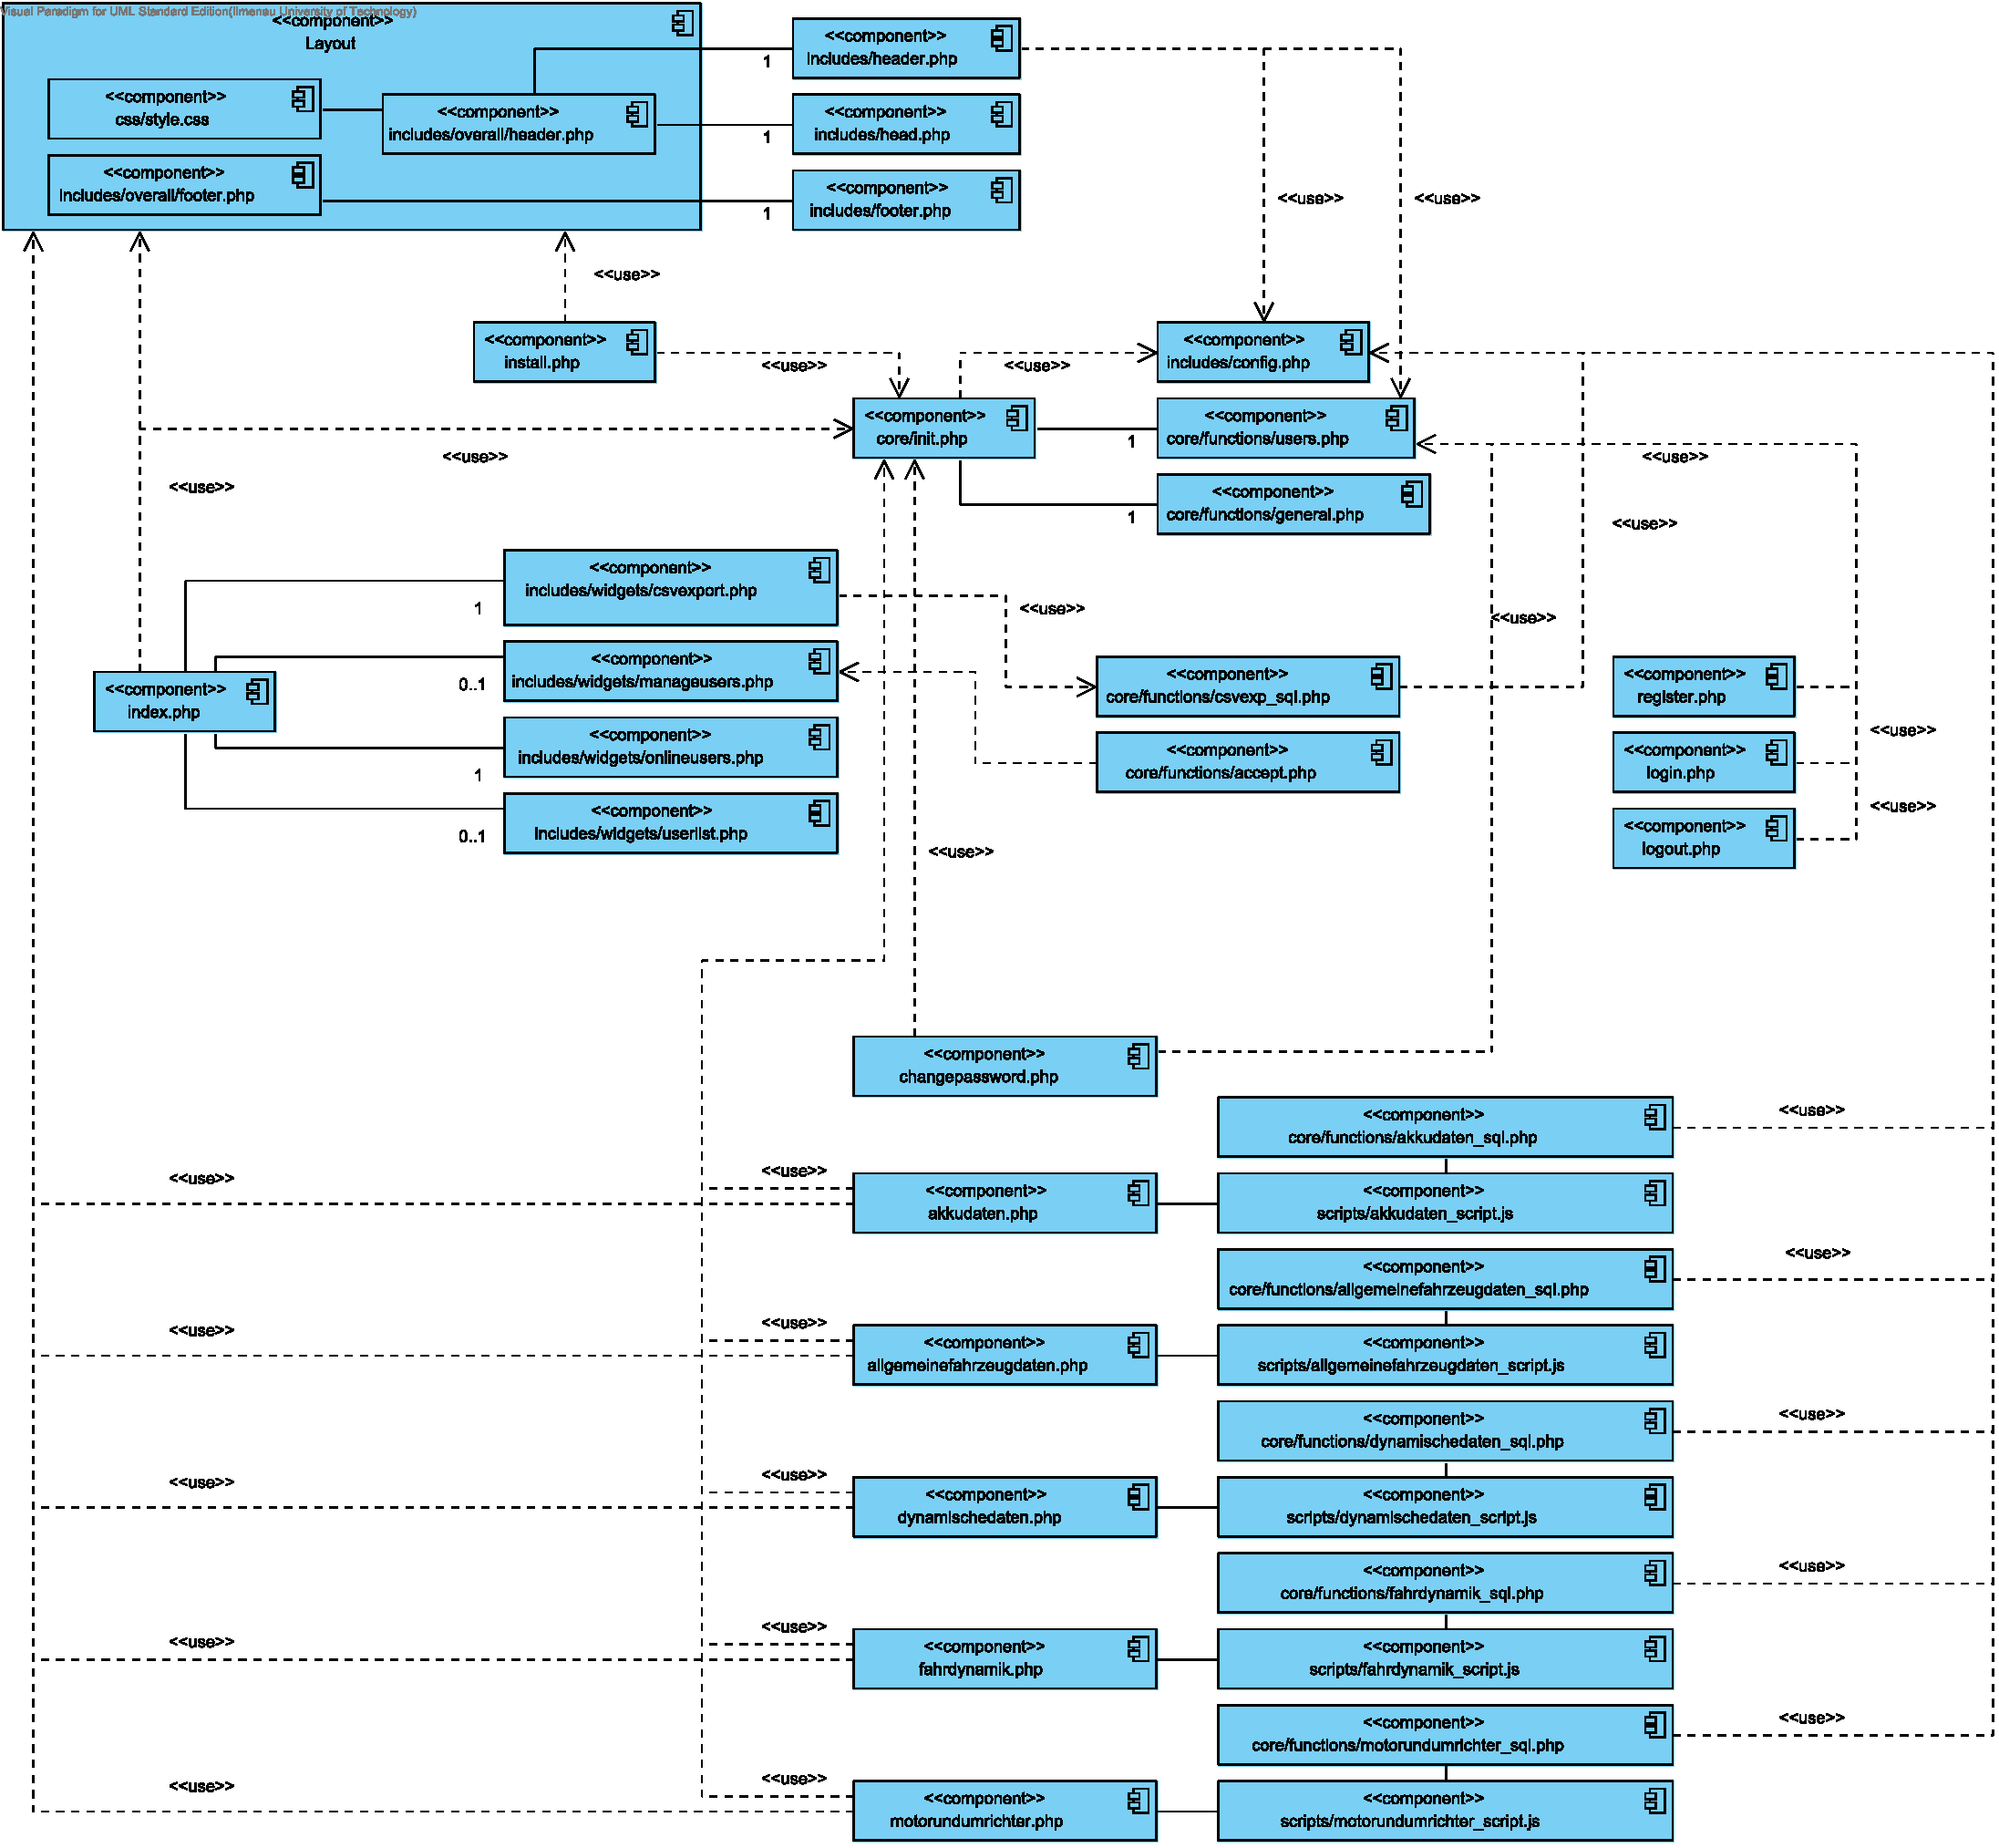
\includegraphics[scale = 0.4]{webseite}
\caption[Komponentendiagramm der Webseite]{Komponentendiagramm der Webseite}
\label{aufbau}
\end{figure}


\subsection{Installation}
Die Installation des Systems wird einmalig und nur beim ersten Besuch der Seite vom Nutzer durchgeführt. Sie wird durch Aufruf der \textit{install.php} gestartet. Hierbei bindet das Skript wie auch alle folgenden selbstständigen Seiten die Dateien \textit{core/init.php}, \textit{includes/overall/header.php, includes/config.php} und \textit{includes/overall/footer.php} ein. In diesen Dateien befinden sich neben \glqq globalen\grqq (es handelt sich hierbei um keine wirklichen PHP-globalen Variablen, sondern lediglich solche, die in allen Skripten verfügbar sind, die \textit{core/init.php} bzw. \textit{includes/config.php} einbinden) Variablendefinitionen auch selbstdefinierte Funktionen. An dieser Stelle ist insbesondere die Funktion \textit{install\_system()} aus der Datei \textit{core/functions/general.php} zu erwähnen (siehe Eintrag zu \textit{general.php}).\\
Der Nutzer wird nach dem Durchlauf des Skripts aufgefordert ein Formular auszufüllen. Mit diesen Daten wird dann der Vorstands-Account (= Admin-Account) erzeugt. Anschließend werden alle benötigten Datenbanken, Tabellen und Einträge erzeugt und das Skript anschließend mittels \textit{exit()} terminiert.

\begin{figure}[h]
\centering
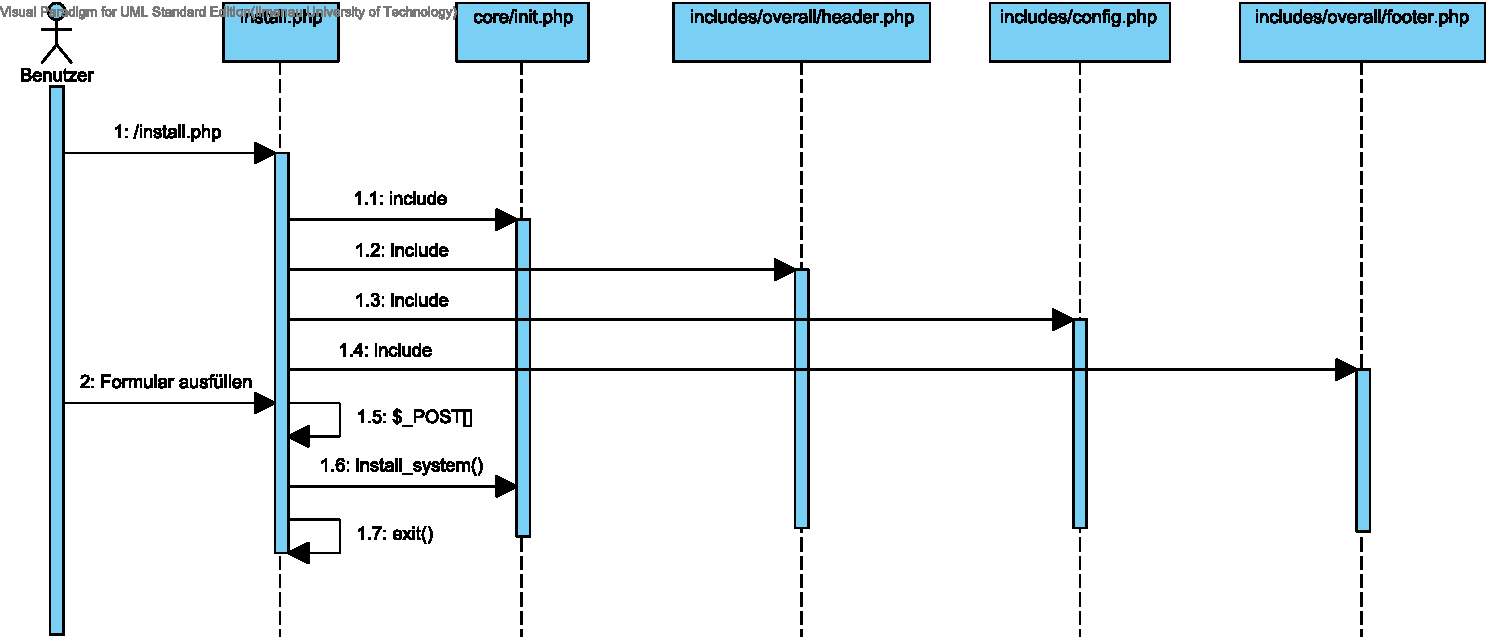
\includegraphics[scale = 0.6]{installation}
\caption[Sequenzdiagramm f\"{u}r den Installationsprozess]{Sequenzdiagramm f\"{u}r den Installationsprozess}
\label{install}
\end{figure}

\newpage
\subsection{Initialisierung der Seiten}
Zu Beginn jeder Seite wird die Datei \textit{core/init.php} eingebunden. Diese sorgt dafür, dass zu Beginn der einzelnen Skripte alle Variablen und Funktionen definiert sind, sowie eine neue Sitzung (Session) gestartet wird. Dies wird erreicht, indem die Dateien \textit{include/config.php}, \textit{core/functions/general.php} und \textit{core/functions/users.php} eingebunden werden. Zudem wird für einige Funktionen bereits eine Verbindung zur Datenbank aufgebaut.\\
Anschließend wird die Funktion \textit{logged\_in()} ausgeführt, diese überprüft ob der Nutzer sich bereits eingeloggt hat. Ist dies nicht der Fall, wird lediglich ein \glqq globales\grqq Array \textit{\$errors[]} erzeugt, indem an vielen Stellen in unterschiedlichen Skripten Fehlermeldungen gesammelt werden können. Hat sich der Benutzer jedoch bereits eingeloggt wird noch geprüft ob der Nutzer bereits aktiviert wurde. Falls nicht, wird die aktuelle Sitzung zerstört, der Benutzer auf die Startseite mittels \textit{header()}-Redirect umgeleitet und das Skript beendet. Ist der Nutzer hingegen bereits aktiviert worden, wird ebenfalls das \glqq globale\grqq Fehlerarray \textit{\$errors[]} angelegt und das Skript beendet.

\begin{figure}[h]
\centering
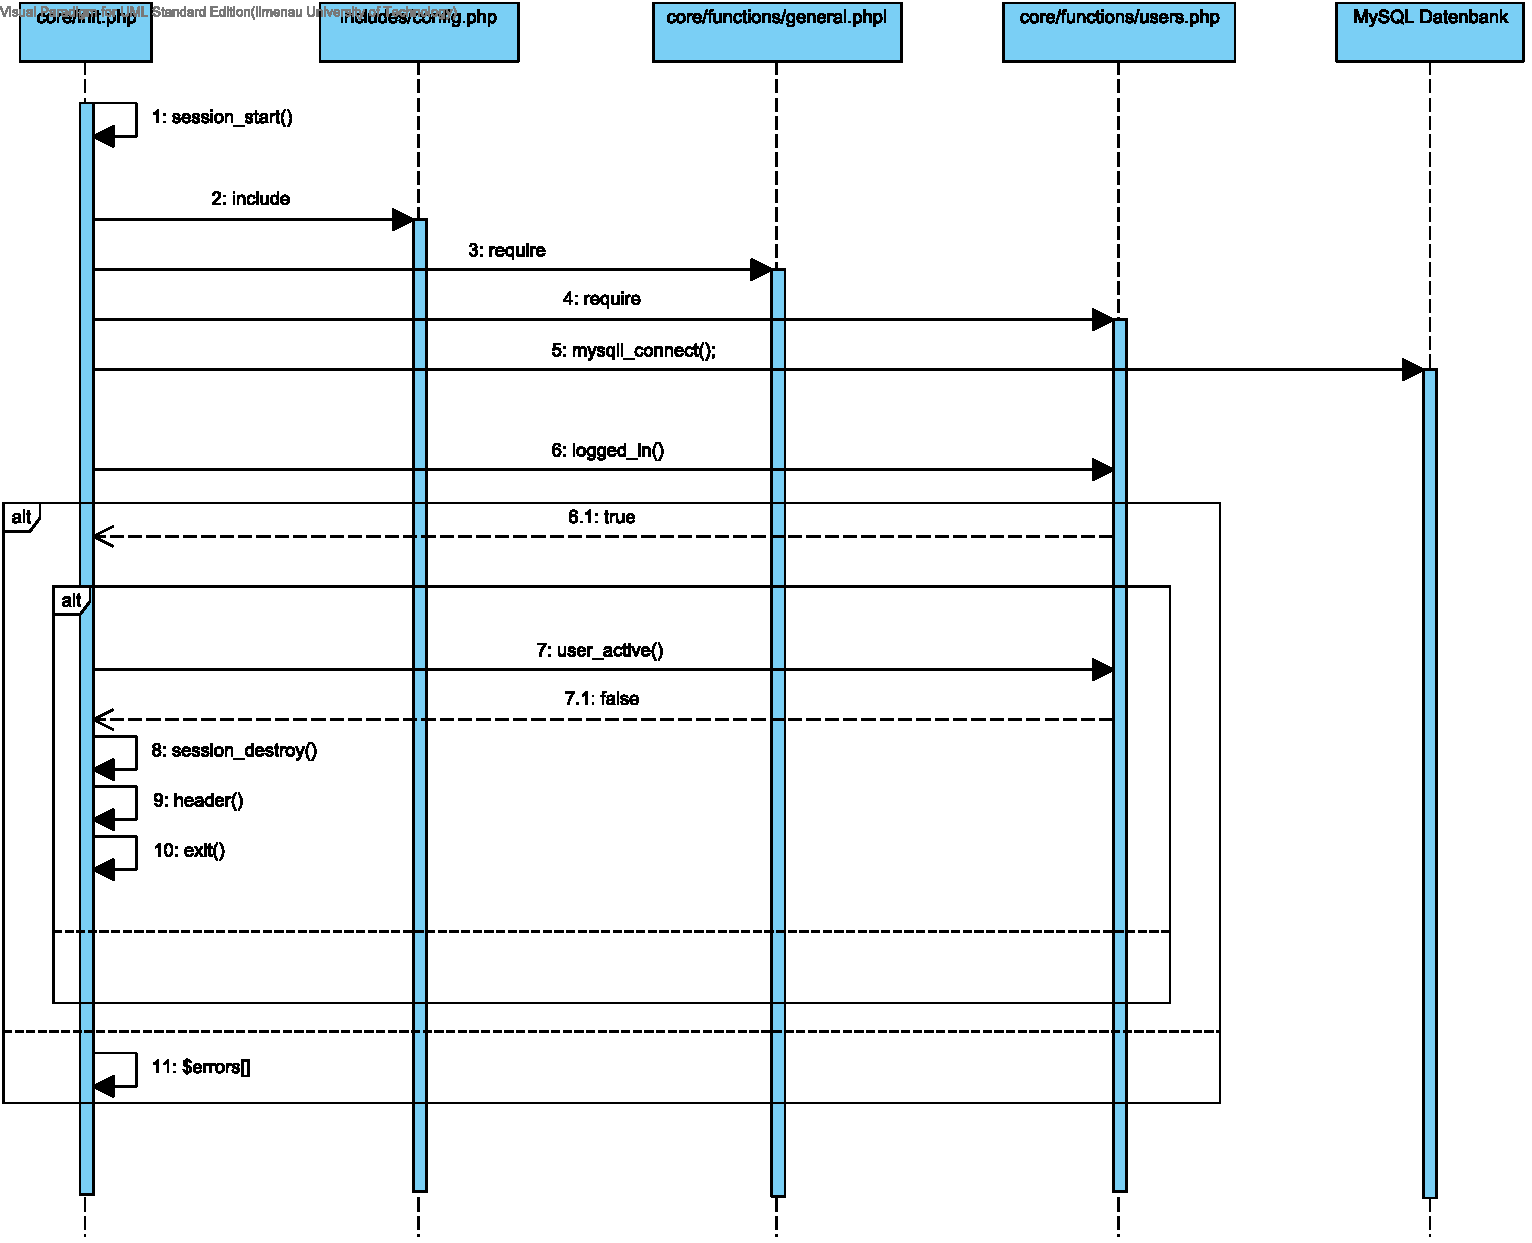
\includegraphics[scale = 0.55]{initialisierung}
\caption[Sequenzdiagramm f\"{u}r die Initialisierung]{Sequenzdiagramm f\"{u}r die Initialisierung}
\label{init}
\end{figure}

\newpage
\subsection{Header}
Die Datei \textit{includes/header.php} wird von der \textit{includes/overall/header.php} eingebunden. Sie setzt vor allen Ding das Menü um, mittels welchem der Nutzer auf der Seite navigieren kann, insofern er denn eingeloggt ist.\\
Dabei prüft \textit{header.php} zuerst mittels der Funktion \textit{logged\_in()} ob der Nutzer eingeloggt ist. Ist dem so, so zeigt er sowohl Menü als auch das Widget \textit{includes/widgets/loggedin.php} an, welches den Nutzer mit seinem Namen begrüßt, ihm die Möglichkeit bietet sein Passwort zu ändern oder die Startseite aufzurufen. Außerdem wird auf den einzelnen Seiten die über das Menü aufgerufen werden können, jeweils eine Information eingeblendet, ob die Daten bereits\glqq veraltet\grqq sind.\\
Desweiteren wird bei Aufruf dieser \textit{header.php} Datei immer der Eintrag in der Online-Nutzer Tabelle aktualisiert, indem die Funktion \textit{refresh()} ausgeführt wird.

\begin{figure}[h]
\centering
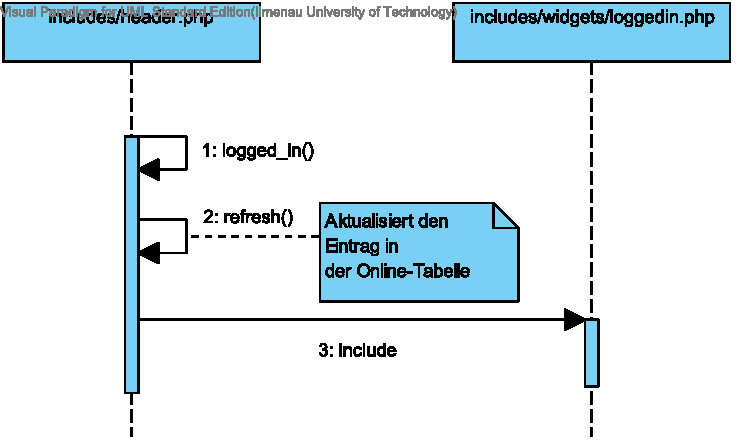
\includegraphics[scale = 1]{header}
\caption[Sequenzdiagramm der Headerdatei]{Sequenzdiagramm der Headerdatei}
\label{header}
\end{figure}

\subsection{Startseite}
Die Startseite ist wie der Name bereits verrät der Startpunkt jedes Aufrufes des Service Interfaces. Nachdem der Benutzer die Seite aufruft werden vom \textit{index.php}-Skript alle nötigen Dateien eingebunden. Die logischen und funktionalen Aspekte werden durch Einbinden der \textit{core/init.php} Datei erreicht. Für das Layout und die HTML-Komponenten wird \textit{includes/overall/header.php} eingebunden (siehe x.y.z Allgemeiner Seitenaufbau [Davids erster Punkt]) wo u. a. auch geprüft wird, ob sich der Nutzer eingeloggt hat oder nicht und ggf. auf die Startseite weitergeleitet wird.\\
Im Anschluss wird überprüft ob sich der Benutzer bereits eingeloggt hat oder nicht. Für den Fall, dass er noch nicht eingeloggt ist, erscheint ein Formular in welches er E-Mail-Adresse und Passwort eingeben kann. Diese Daten werden anschließend an das Skript \textit{login.php} mittels \textit{POST}-Request verschickt und anschließend validiert sowie verifiziert (siehe x.y.z).\\
Alternativ kann sich der Benutzer auch einen neuen Account erstellen. Dies erreicht er durch Auswählen des \glqq Jetzt registrieren\grqq-Links, wodurch er auf die Skript-Seite \textit{register.php} weitergeleitet wird. Der Nutzer erhält erneut ein Formular, welches er für die Registrierung vollständig ausfüllen muss. Diese Daten werden anschließend nach dem Klick auf den Abschicken-Button validiert (siehe x.y.z.).\\
Hat sich der Nutzer eingeloggt oder war bereits eingeloggt als er die Seite aufrief, werden ihm anstelle des Login-Formulars einige Widgets in Abhängigkeit seiner Rechtegruppe (\textit{isVorstand()}-Aufruf) angezeigt, die da wären

\begin{itemize}
 \item Möglichkeit zum Export der in der Datenbank befindlichen Fahrzeugdaten (jeder Nutzer; \textit{includes/widgets/csvexport.php})
 \item Liste der sich aktuell online befindlichen Nutzer (jeder Nutzer;\\ \textit{includes/widgets/onlineusers.php})
 \item Möglichkeit der Verwaltung der Nutzer\\ (nur Vorstand; \textit{includes/widgets/manageusers.php})
 \item Liste der im System registrierten Benutzer (nur Vorstand; \textit{includes/widgets/userlist.php})
Desweiteren werden ihm nach dem Login auch ein horizontales Menü eingeblendet über welches der Nutzer die Möglichkeit erhält die verschiedenen Unterseiten aufzurufen und sich ggf. wieder auszuloggen.
\end{itemize}

\begin{figure}[h]
\centering
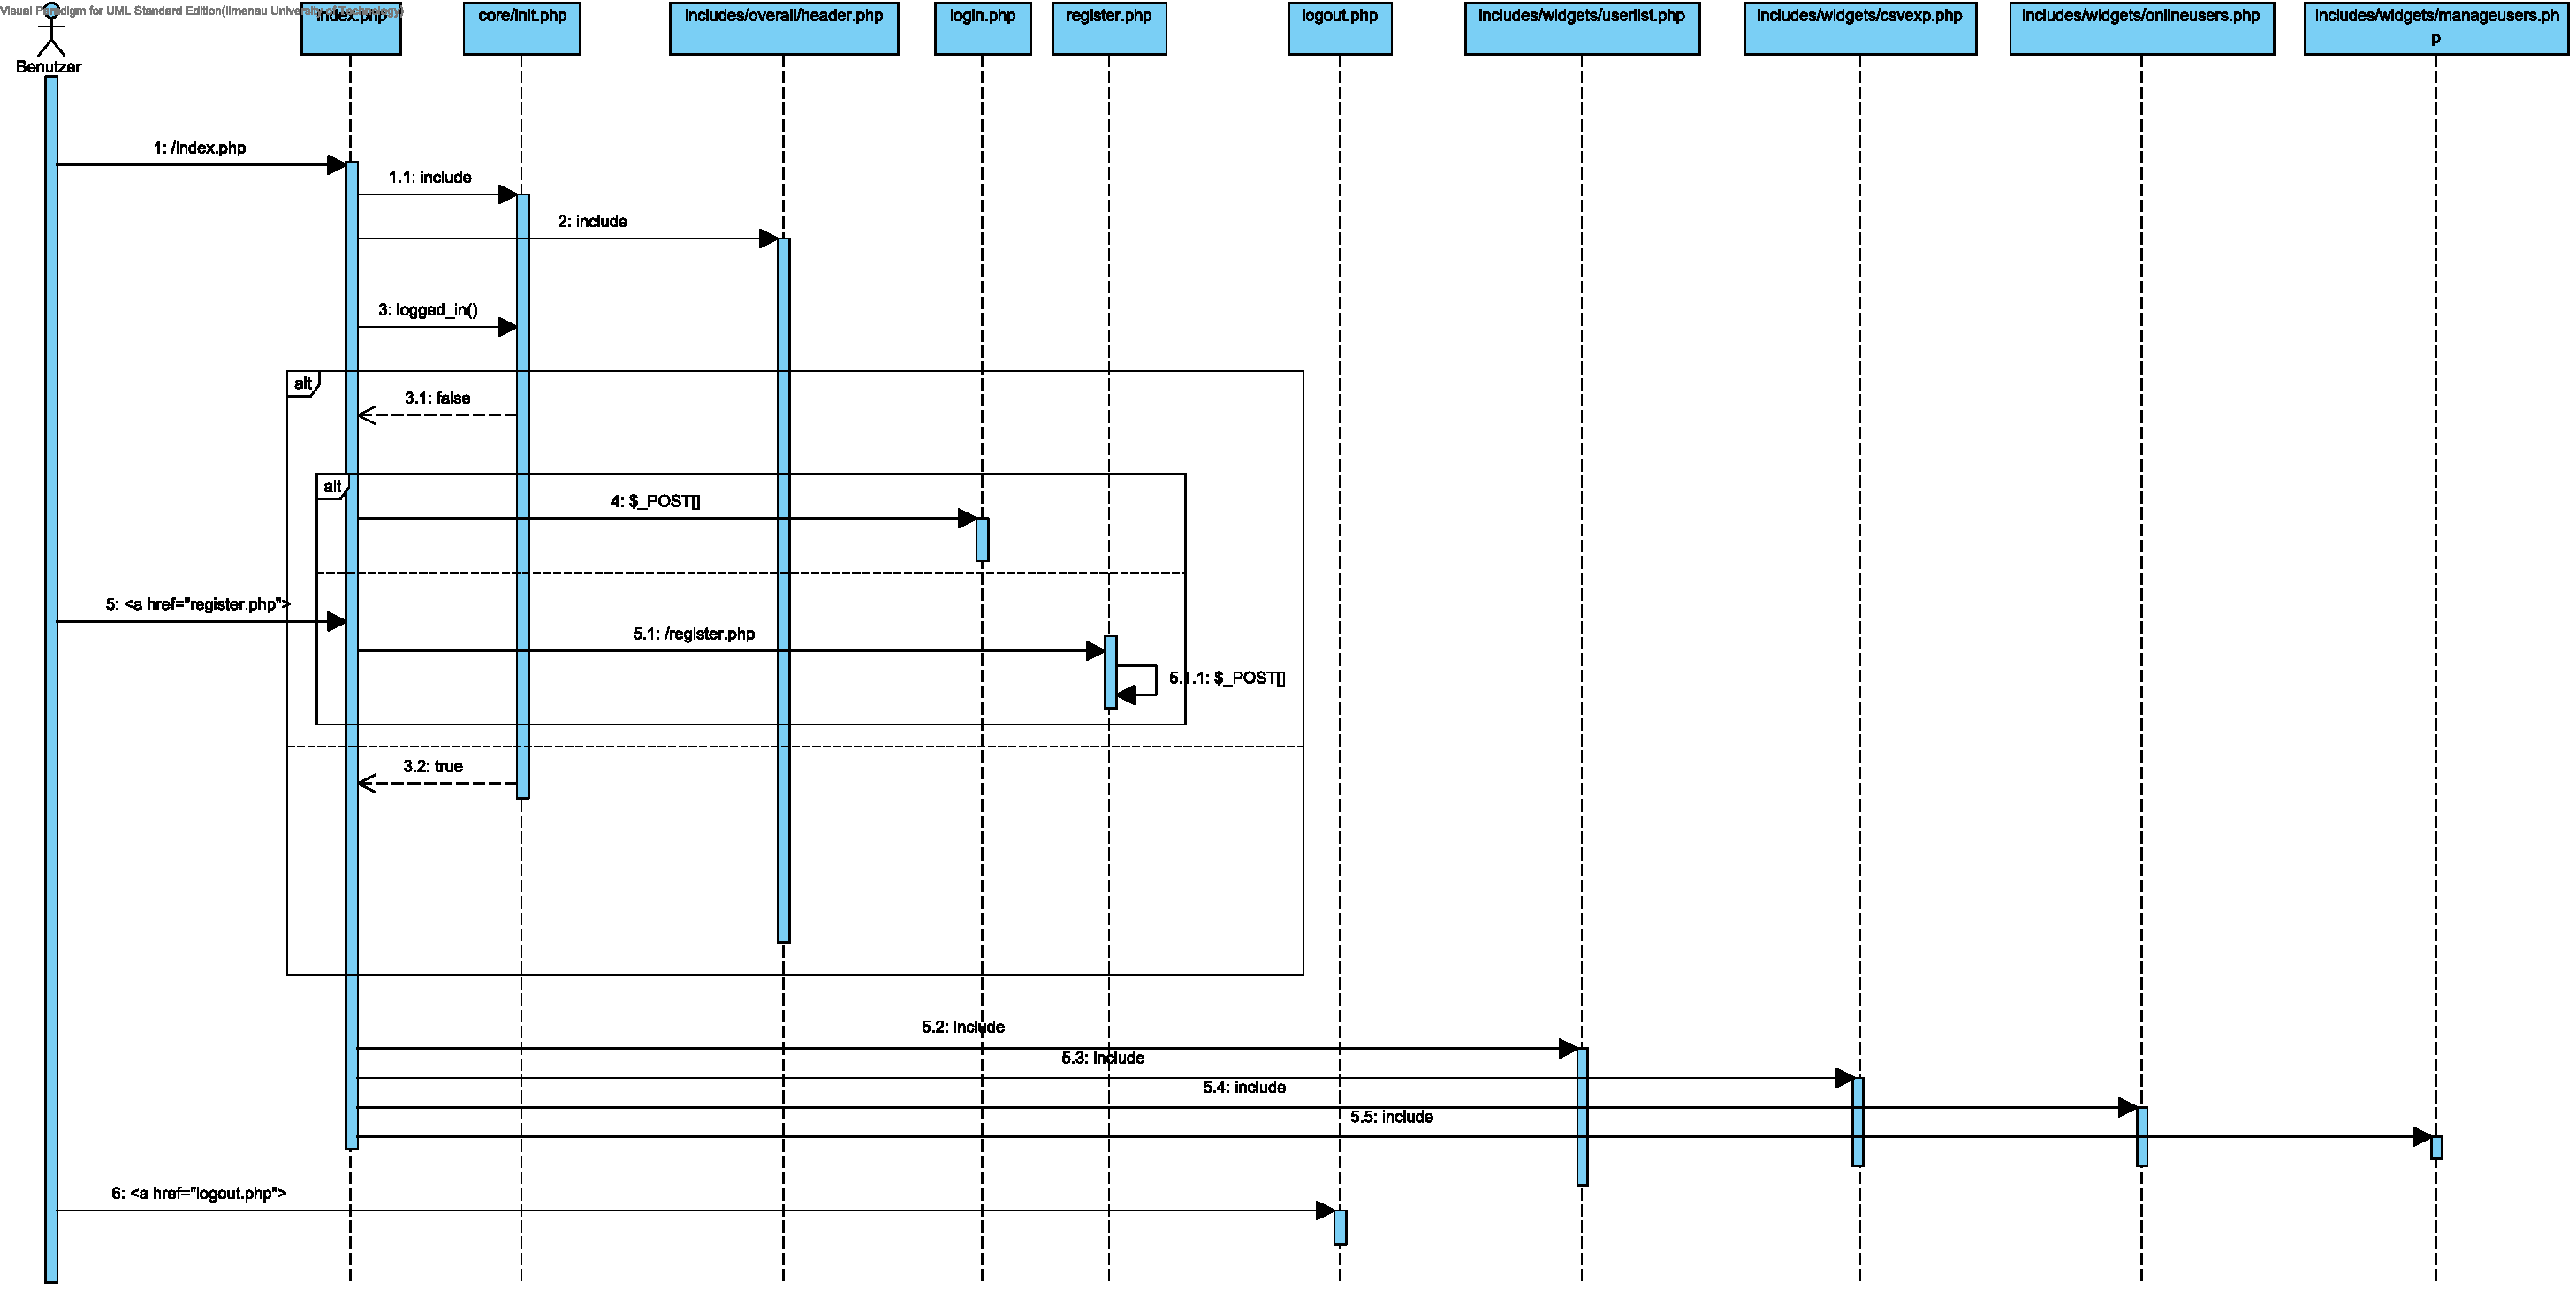
\includegraphics[scale = 0.315]{startseite}
\caption[Sequenzdiagramm der Startseite]{Sequenzdiagramm der Startseite}
\label{index}
\end{figure}

\newpage
\subsection{Registrierung}
Der Nutzer erreicht über einen Link auf der Startseite das Registrierungsformular. Dieses bindet zu Beginn die gewohnten \textit{includes/overall/header.php} und die \textbf{core/init.php} ein. Anschließend wird geprüft ob der Nutzer sich bereits eingeloggt hat. Falls ja, so wird er auf die Startseite umgeleitet, andernfalls wird ihm das Registrierungsformular angezeigt. Dieses muss er vollständig ausfüllen, damit seine Registrierungsanfrage verarbeitet wird. Die eingegeben Daten werden mittels POST-Request an sich selbst geschickt, validiert und anschließend ein neuer Eintrag in der Benutzertabelle angelegt. Dabei wird der Status des Nutzer standardmäßig auf \textit{0}, d.h. \textit{deaktiv}, gesetzt. Anschließend wird der Nutzer mittels \textit{header()}-Umleitung erneut auf die Registrierungsseite umgeleitet und das vorhergehende Skript durch Aufruf der \textit{exit()}-Funktion beendet.

\begin{figure}[h]
\centering
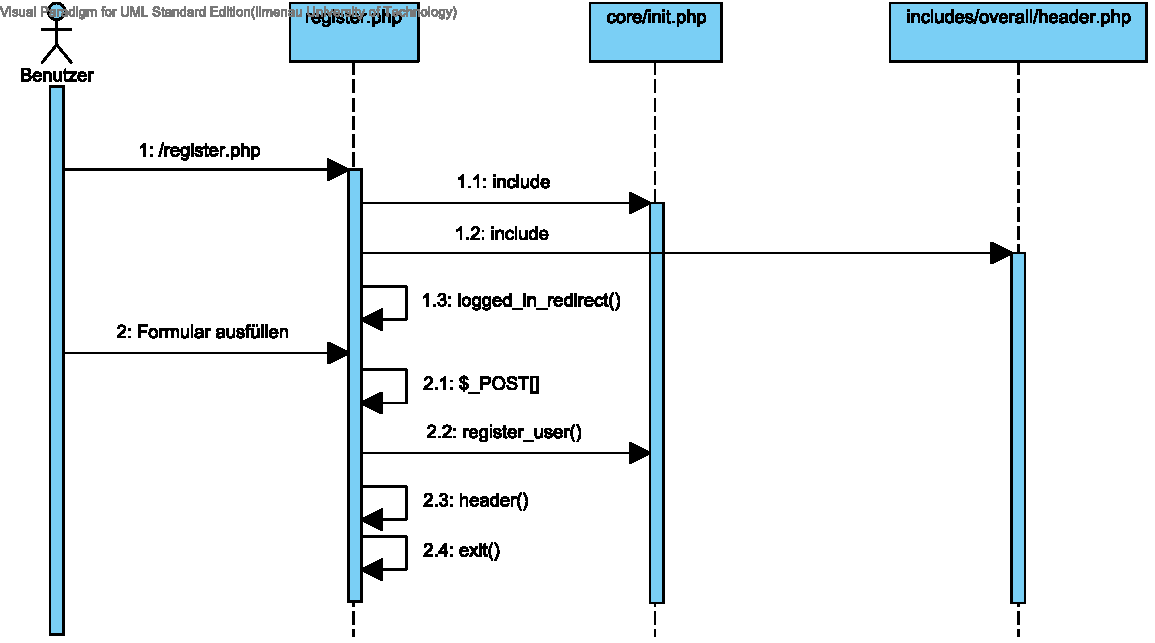
\includegraphics[scale = 0.75]{registrierung}
\caption[Sequenzdiagramm des Registriervorgangs]{Sequenzdiagramm des Registriervorgangs}
\label{registrierung}
\end{figure}

\newpage
\subsection{Loginvorgang}
% LOGIN %
Nach der Eingabe der Login-Daten wird der Nutzer auf die Seite \textit{login.php} weitergeleitet. Das hier ausgeführte Skript bindet wie gewohnt zuerst die allgemeine Initialisierungsdatei \textit{core/init.php} ein, sowie die für das Layout benötigten \textit{includes/overall/header.php} respektive \textit{includes/overall/footer.php} und überprüft ob der Nutzer bereits eingeloggt ist. Ist dies der Fall wird das Skript beendet und er automatisch auf die Startseite weitergeleitet.\\
An sonsten führt das Skript anhand der als \textit{POST}-Request übermittelten Daten eine Anfrage aus und verifiziert die Login-Daten. Bei erfolgreicher Verifizierung werden die Sessionvariablen \textit{\$\_SESSION['user\_id']} und \textit{\$\_SESSION['time']} (aktueller UNIX-Zeitstempel) gesetzt und anschließend eine Verbindung zur Datenbank erzeugt. Nach der Auswahl der benötigten Datenbank wird ein neuer Eintrag in der Online-Tabelle erzeugt, der sich aus der den beiden Session-Variablen zusammensetzt. Anschließend wird der Nutzer auf die Startseite weitergeleitet und die Ausführung des Skripts mittels \textit{exit()} beendet.\\

\begin{figure}[h]
\centering
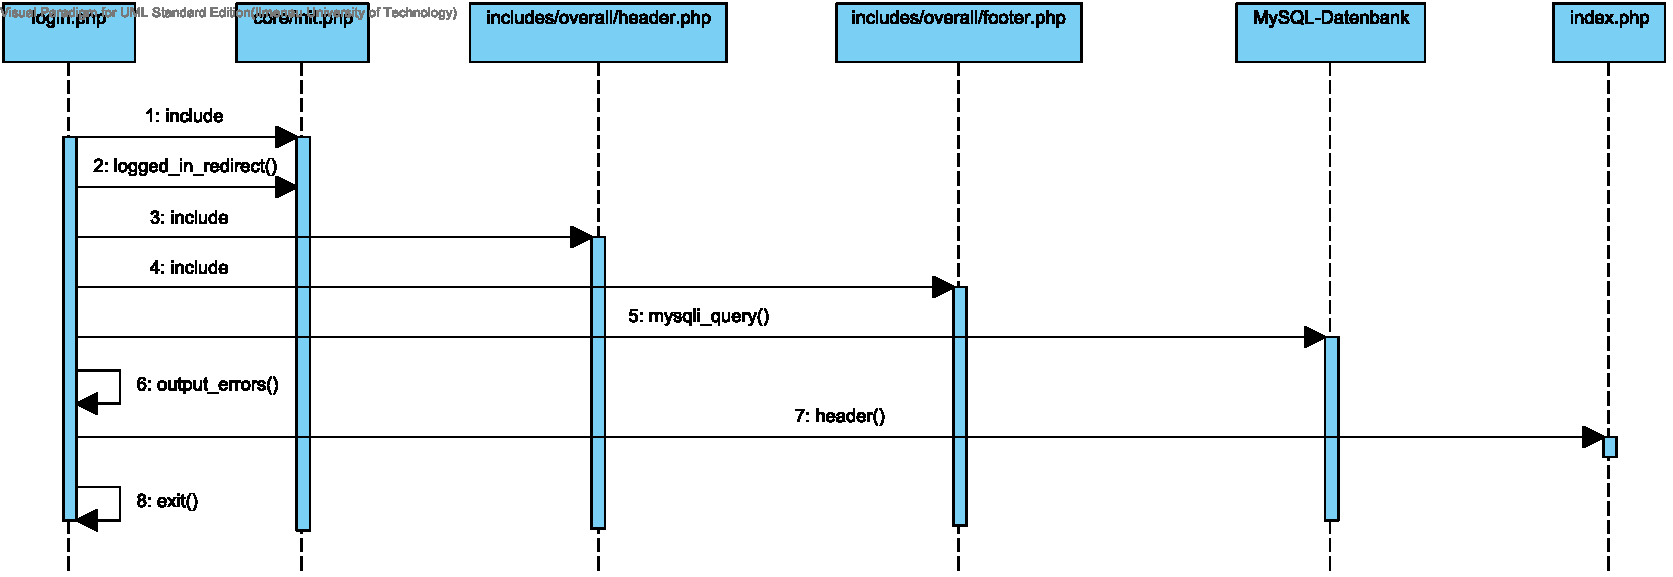
\includegraphics[scale = 0.5]{login}
\caption[Sequenzdiagramm des Loginvorgangs]{Sequenzdiagramm des Loginvorgangs}
\label{login}
\end{figure}

\newpage
\subsection{Logoutvorgang}
% LOGOUT %
Nach Aufruf der \textit{logout.php} Datei wird das \textit{core/init.php} Skript eingebunden, woraufhin es die benötigte Datenbank auswählt und anschließend eine SQL-Anfrage an die MySQL-Datenbank sendet, die den \glqq Online\grqq-Eintrag des aktiven Nutzers löscht. Abschließend wird die aktuelle Sitzung mittels \textit{session\_destroy()} beendet, der Nutzer auf die \textit{index.php} mittels \textit{header()}-Weiterleitung weitergeleitet und das Script beendet.

\begin{figure}[h]
\centering
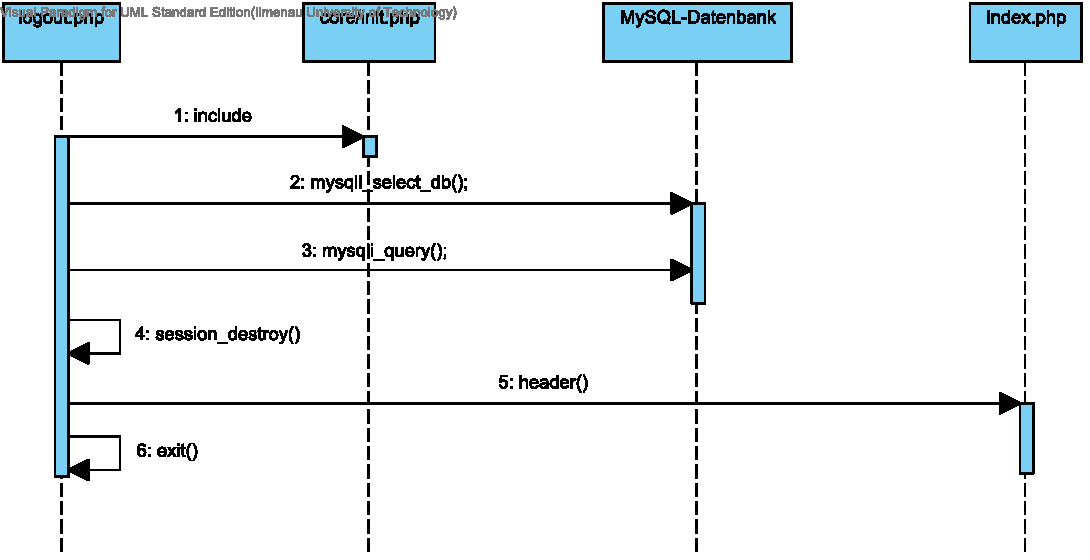
\includegraphics[scale = 0.7]{logout}
\caption[Sequenzdiagramm des Logoutvorgangs]{Sequenzdiagramm des Logoutvorgangs}
\label{logout}
\end{figure}

\newpage
\subsection{Änderung des persönlichen Passworts}
Das Skript \textit{changepassword.php} bindet nach Aufruf zuerst die allgemeine \textit{core/init.php} Datei, sowie die für das Layout verantwortliche \textit{includes/overall/header.php} und \textit{include/overall/footer.php} ein und überprüft das Skript ob die aufrufende Person bereits eingeloggt ist.\\
Der Benutzer kann durch Ausfüllen des ihm an dieser Stelle zur Verfügung gestellten Formulars durch Eingabe seines bisherigen Passworts und seines neuen Passworts (inkl. Wiederholung) ändern. Nach dem Abschicken des Formulars werden die Daten validiert und nach erfolgreicher Validierung durch Aufruf der \textit{change\_password()}-Funktion persistent im System gespeichert. Anschließend wird der Benutzer zurück mittels \textit{header()}-Umleitung auf die \textit{changepassword.php}-Seite geführt.

\begin{figure}[h]
\centering
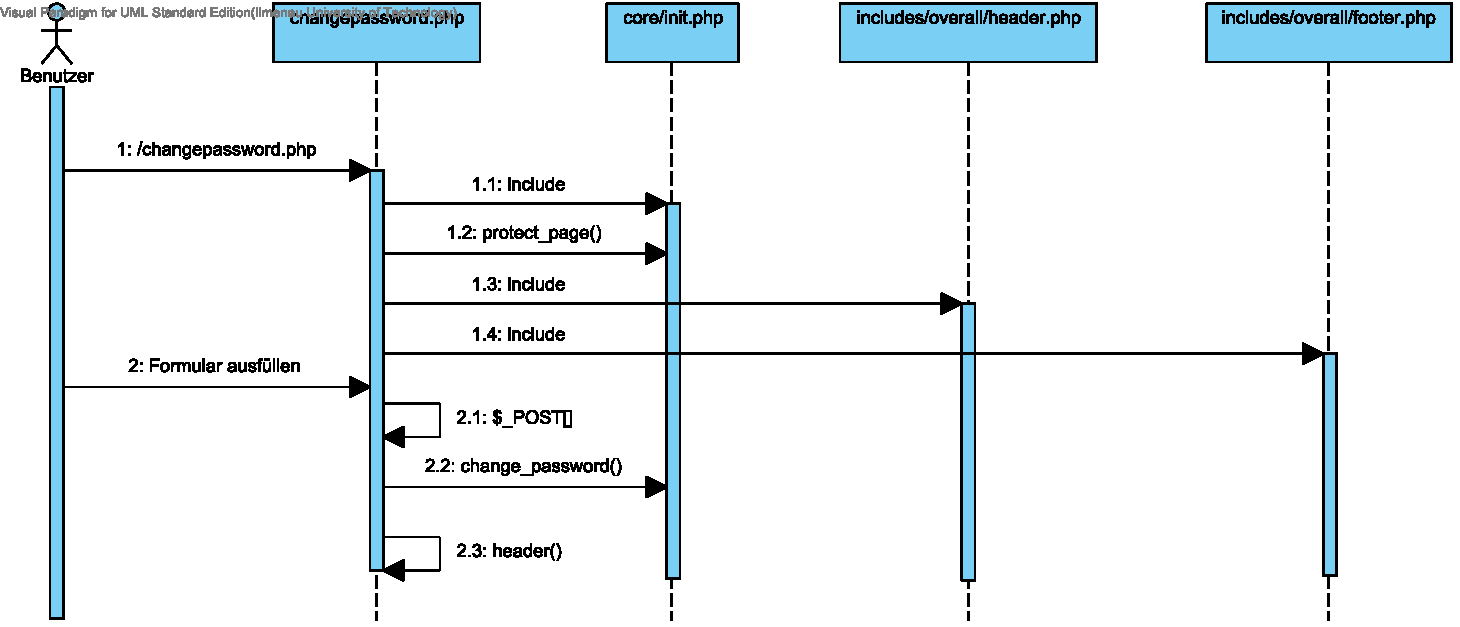
\includegraphics[scale = 0.6]{passwort}
\caption[Sequenzdiagramm der Passwort\"{a}nderungsfunktion]{Sequenzdiagramm der Passwort\"{a}nderungsfunktion}
\label{passwort}
\end{figure}

\newpage
\subsection{CSV-Exportfunktionalität}
Wird ebenfalls als Widget für die Startseite angeboten. Dieses stellt eine Liste von Checkboxen zur Verfügung. Durch Auswahl der einzelnen Checkboxen können die zu exportierenden Tabellen gewählt werden. Die Auswahl wird mittels POST-Request an die Datei \textit{core/functions/csvexp\_sql.php} gesendet, welche dann eine Verbindung zum MySQL-Server aufbaut, die Datenbank auswählt und die gewünschte Abfrage ausführt. Anschließend wird die Verbindung geschlossen und dem Benutzer öffnet sich ein Fenster, dass ihm zum Download der nun erstellen CSV-Datei auffordert.

\begin{figure}[h]
\centering
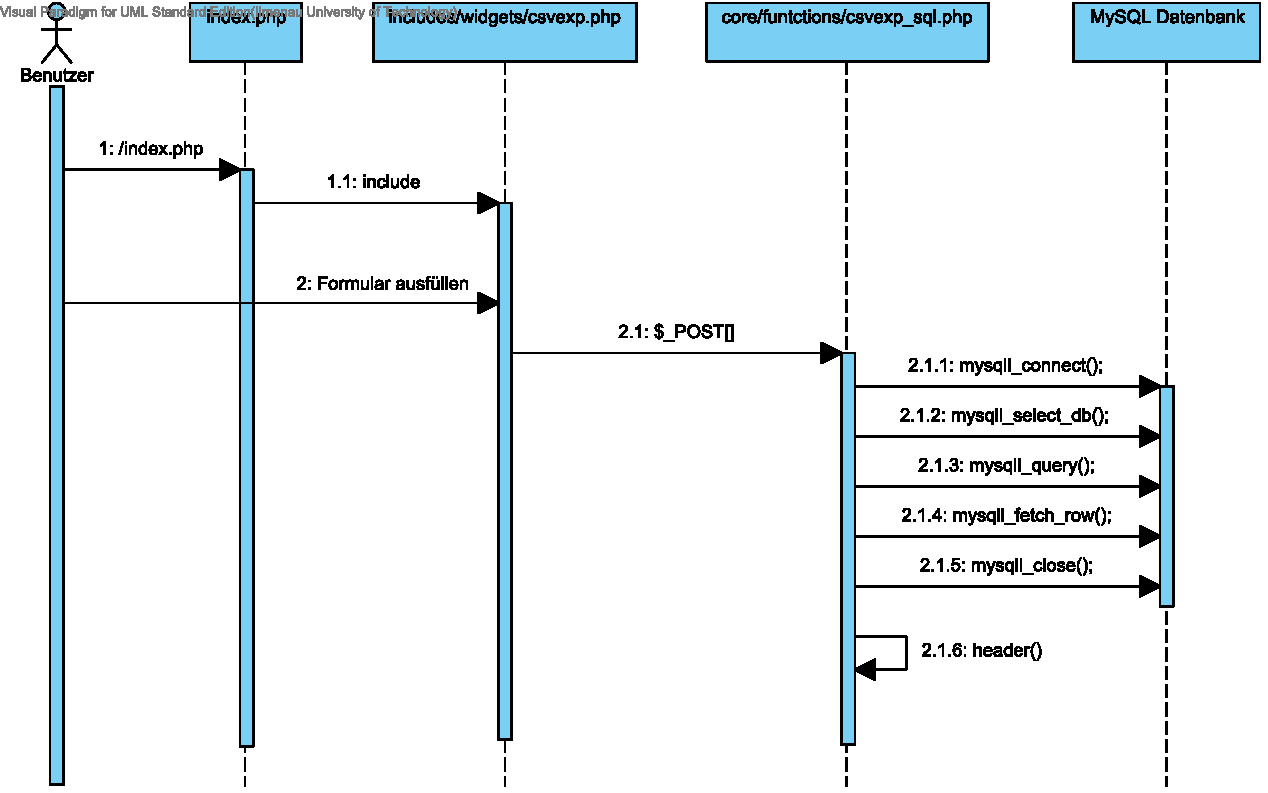
\includegraphics[scale = 0.6]{csvexport}
\caption[Sequenzdiagramm des CSV-Export]{Sequenzdiagramm des CSV-Export}
\label{csv}
\end{figure}

\newpage
\subsection{Nutzerverwaltung}
Hierbei handelt es sich um genau zu sein um zwei Widgets (\textit{includes/widgets/manageusers.php} und \textit{includes/widgets/userlist.php}), welche auf der Startseite für eingeloggte Benutzer eingebunden werden. Dabei stellt \textit{userlist.php} die im System bereits registrierten Nutzer dar. Hierfür baut das Skript eine Verbindung zur Datenbank auf, wählt die Tabelle der registrierten Nutzer aus (ID, Vorname, Nachname, E-Mail-Adresse, Rechtegruppe, Account-Status) und gibt diese als HTML-Tabelle aus. Die zweite Datei, \textit{manageusers.php}, bietet dem Nutzer ein Formular an, das auf Eingabe einer Nutzer-ID (entnehmbar der Nutzerliste, s.o.), der Auswahl ob der Nutzer aktiviert oder gelöscht werden soll, durch Auswählen einer der beiden Radioboxen, sowie der Wahl einer der drei voreingestellten Benutzergruppen mittels einer Dropdown-Box, ein Skript (\textit{core/functions/accept.php}) aufruft, welches die übergebenen Daten validiert und anschließend die Änderungen durch Aufbau einer Verbindung zur Datenbank in der Benutzertabelle persistent speichert. Am Ende des Skripts wird der Nutzer automatisch mittels \textit{header()}-Weiterleitung zurück auf die Startseite befördert.

\begin{figure}[h]
\centering
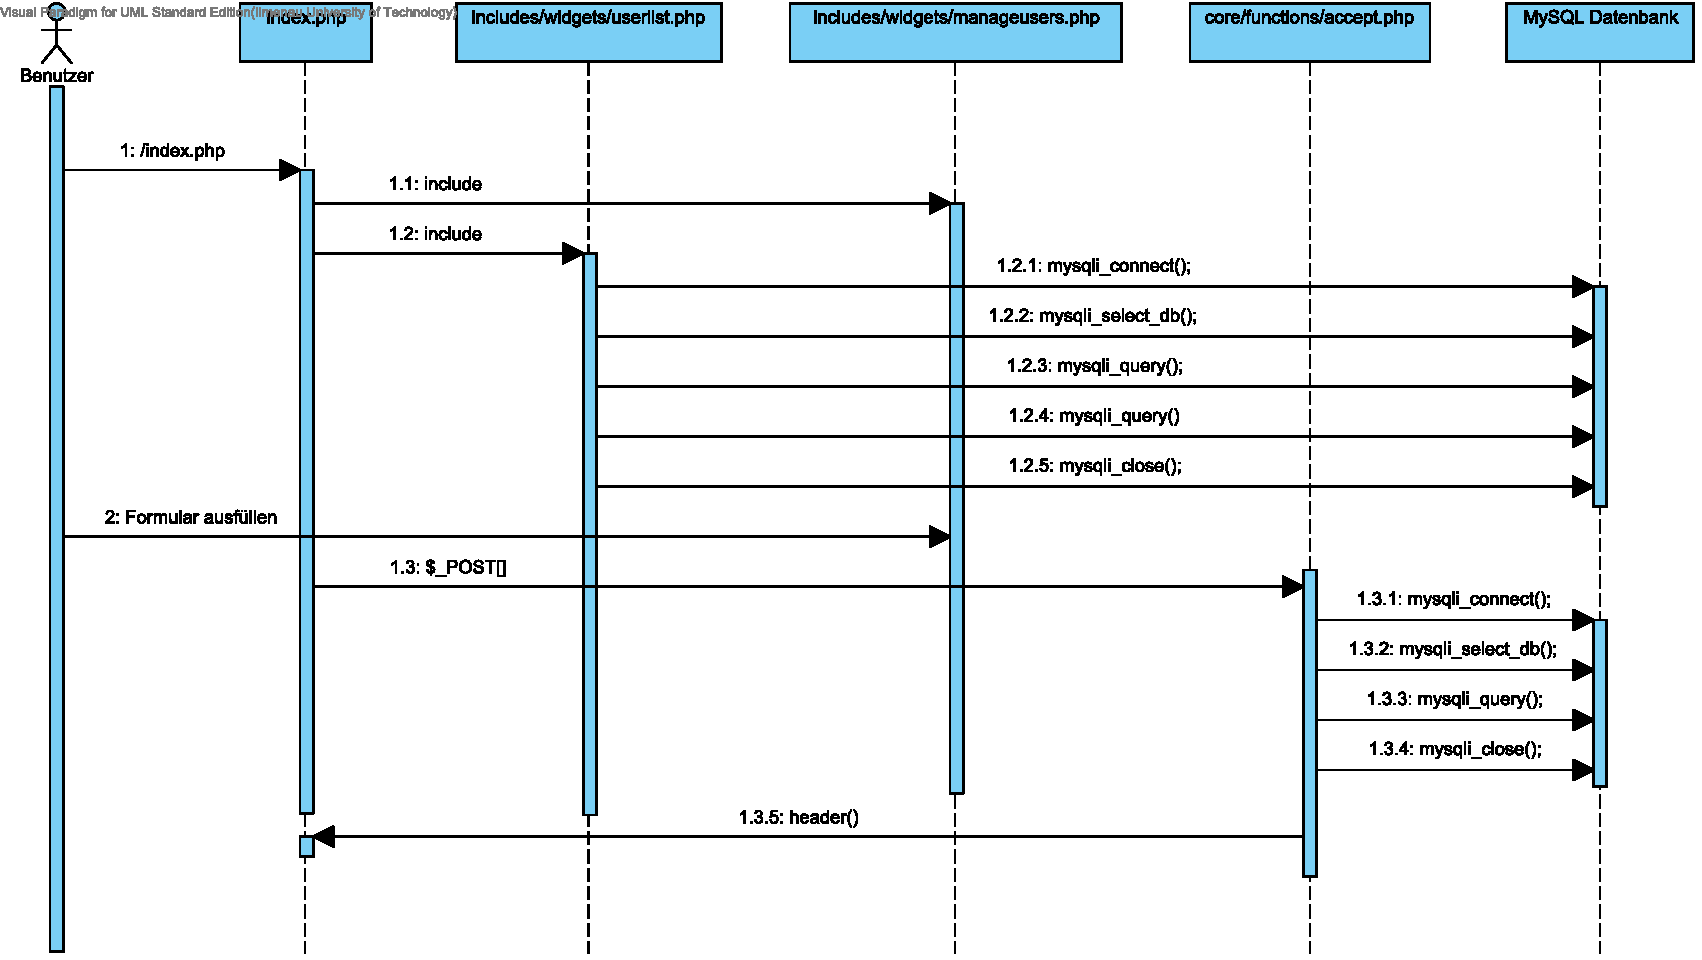
\includegraphics[scale = 0.5]{usermgmt}
\caption[Sequenzdiagramm der Benutzerverwaltung]{Sequenzdiagramm der Benutzerverwaltung}
\label{usermgmt}
\end{figure}

\newpage
\subsection{Online-Anzeige der Nutzer}
Hierbei handelt es sich um ein kleines Widget, welches nicht mehr tut, als dass es eine festgelegte SQL-Anfrage an den MySQL-Server stellt. Dabei wird wie gewohnt zuerst die Verbindung eröffnet, die Datenbank ausgewählt und anschließend die Anfrage auf dieser ausgeführt. Das zurückgegebene Ergebnis wird anschließend als HTML-Tabelle ausgegeben und die Verbindung zum MySQL-Server wieder geschlossen.

\begin{figure}[h]
\centering
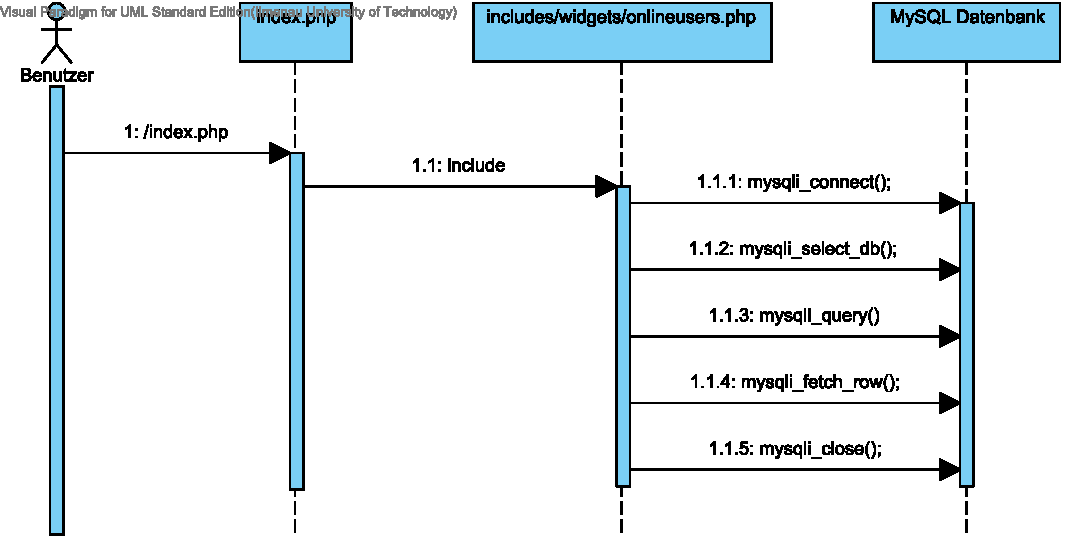
\includegraphics[scale = 0.8]{online}
\caption[Sequenzdiagramm der Onlineanzeige]{Sequenzdiagramm der Onlineanzeige}
\label{online}
\end{figure}

\newpage

%%%%%%%%%%%%%%%%%%% KUDA FEINENTWURF %%%%%%%%%%%%%%%%%%%%%%%%%%%%%%%%


\subsection{Allgemeine Seitenaufbau}
Im allgemeinen Seitenaufbau geht es um eine Folge von Seitenaufrufen, Funktionen und Einbindevorgänge. Diese sind für die 5 darstellenden Seiten identisch und werden deshalb an dieser Stelle zusammenfassend veranschaulicht.
\\ \\
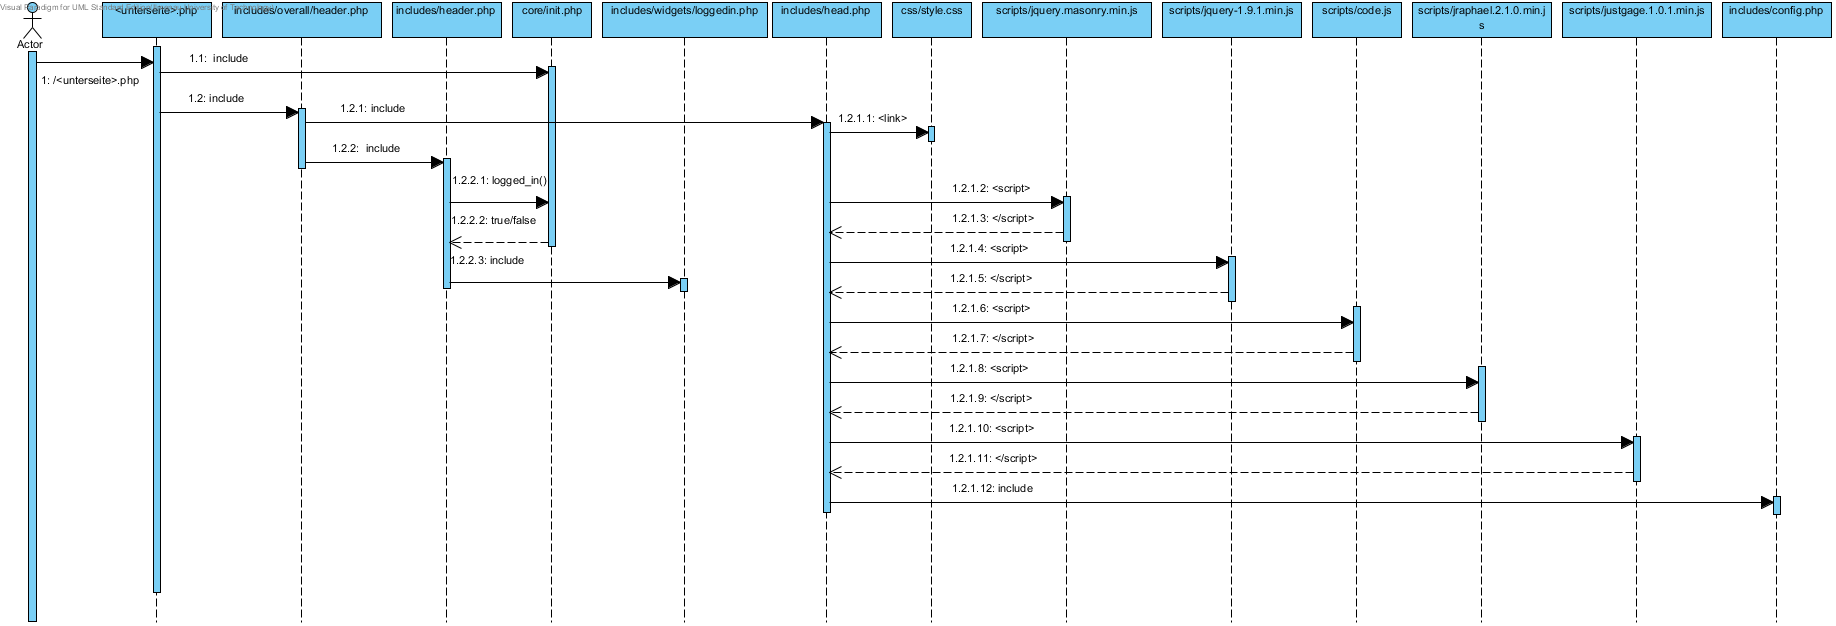
\includegraphics[scale=0.327]{allgemeineSeitenaufbau.png}
\\ \\

\textbf{includes/overall/header.php}\\
\hangindent+95pt \hangafter=1
Beschreibt den Aufbau des Dokuments. Dabei wird der Dokumenttyp bestimmt, danach der Head-, sowie der Navigationsbereich eingebunden.\\


\textbf{includes/head.php}\\
\hangindent+95pt \hangafter=1
Diese Datei stellt den regulären Headbereich einer Webseite dar. Hier werden alle allgemein nötigen Skripte, CSS-Datein und Seiten importiert. Darunter sind die vier Javascript Bibliotheken: jQuery, justGage, rapheal und masonry, die alle unter der MIT Lizenz frei verfügbar sind. Weiterhin wird die Datei config.php eingebunden, die relevante Informationen zum Zugriff auf die Datenbanken bereithält.\\


\textbf{includes/header.php}\\
\hangindent+95pt \hangafter=1
Beinhaltet die Navigationsleiste am Kopf der Seite, die auf allen Seiten präsent ist. An dieser Stelle wird auch geprüft, ob der Nutzer angemeldet ist. Die Navigationsleiste wird nur angemeldeten Nutzern angezeigt.





\subsection{Allgemeine Fahrzeugdaten}
Auf dieser Seite werden die im Pflichtenheft vereinbarten allgemeinen Daten dargestellt. Darunter fällt die Geschwindigkeit, die als Halbkreis-Diagramm mittels der JavaScripte justGage und raphael realisiert wird. Die Notausschalter werden als Tabelle dargestellt , wobei ein aktivierter Schalter farblich in rot hinterlegt wird. Die Seite enthält drei wesentliche Dateien: Die PHP-Seite, die den strukturellen Aufbau beinhaltet (allgemeinefahrzeugdaten.php), das Javascript was in die Seite eingebunden und ausgeführt wird (allgemeinefahrzeugdaten\_script.js), sowie eine PHP-Seite, die die MySQL Anfrage für die Seite realisiert (allgemeinefahrzeugdaten\_sql.php). 
\\ \\
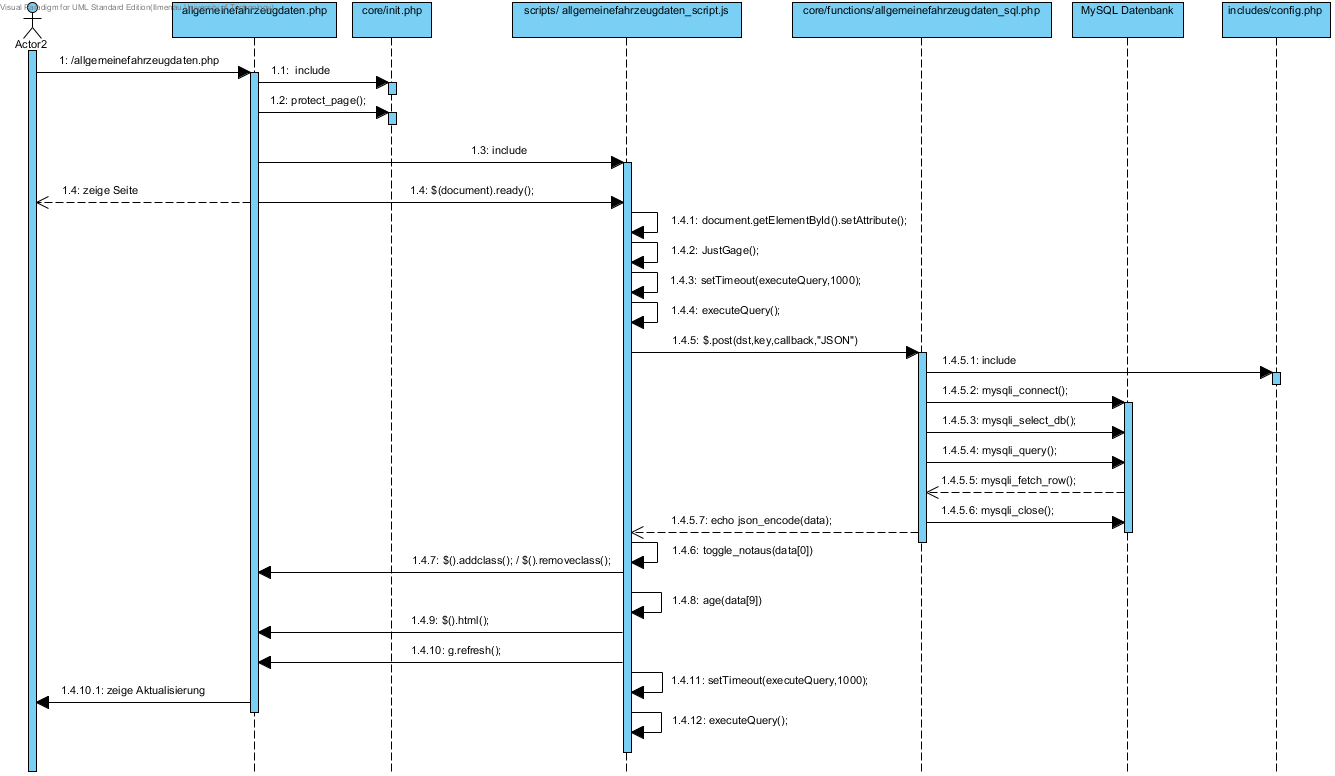
\includegraphics[scale=0.452]{allgemeinefahrzeugdaten.png}
\\ \\


\textbf{protect\_page()}
\hspace{0.5mm}
\hangindent+95pt \hangafter=1 Diese Funktion aus der "'init.php"' wird verwendet, um den unberechtigten Zugriff auf die Seite zu vermeiden und den Nutzer auf die Login-Seite weiterzuleiten.\\


\textbf{\$(document).ready()}\\
\hangindent+95pt \hangafter=1 
Wenn die Seite komplett aufgebaut ist, wird dies Aktion ausgeführt und startet weitere Funktionen des JavaScripts. \\


\textbf{document.getElementByID().setAttribute}\\
\hangindent+95pt \hangafter=1  
Ein Aufruf, der bewirkt, dass alle Klassen der Navigationsbuttons verändert werden. Wird 5 mal ausgeführt, wobei alle nicht ausgewählten Schaltflächen grau werden und der ausgewählte Button färbt sich blau. \\


\textbf{justGage()}
\hspace{9mm}
\hangindent+95pt \hangafter=1 
Initialisiert die halbrunde Geschwindigkeitsanzeige, die durch \textbf{"'g.refresh()"'} aktualisiert wird. \\


\textbf{setTimeout(executeQuery,1000)}\\
\hangindent+95pt \hangafter=1 
Dieses Timeout realisiert die Aktualisierung im Sekundentakt. Dabei sorgt der erste Aufruf dafür, dass "'executeQuery()"' zum ersten mal aufgerufen wird und jeder weitere Aufruf (innerhalb von "'executeQuery()"') sorgt dafür, das die Funktion kontinuierlich wiederholt wird.\\ 


\textbf{executeQuery()}\\
\hangindent+95pt \hangafter=1 
Aufgabe dieses Aufrufs ist Anforderung des JSON-Arrays, sowie das erneute Selbstaufrufen durch einen Timeout.\\


\textbf{\$.post('allgemeinefahrzeugdaten\_sql.php',\{permission:"true"\},function(data)\{\} ,"JSON")}\\
\hangindent+95pt \hangafter=1 
Dies Funktion ruft die an erster Stelle genannte Seite auf und erwartet als Rückgabe ein Array (data). JSON ist dabei die vereibarte Notation (Java Script Object Notation). In diesem Array stehen dann der Reihe nach alle aktuellen Werte aus der Datenbank. Des weiteren wird ein array mit einem Wert zusätzlich an die Seite gesendet (Position= permission, Wert=true), die bewirkt, dass kein unbefugter durch direkte Eingabe der Seite den Datensatz bekommen kann. \\


\textbf{allgemeinefahrzeugdaten\_sql.php}\\
\hangindent+95pt \hangafter=1 
Diese Seite realisiert die jeweilige Datenbankanfrage und wandelt das Ergebnis mit "'json\_encode"' in ein Array um, dass dann an die aufrufende Seite zurückgegeben wird.\\


\textbf{toggle\_notaus(), removeClass/addClass}\\
\hangindent+95pt \hangafter=1 
Der Status der Notausschalter wird als String übergeben. Er besteht aus einer Folge von 0 und 1, der aufgetrennt werden muss. Im Anschluss wird mit "'(ID).removeClass"' und "'(ID).addClass"' jeweils der Status der Schalter (AN/AUS) geändert, und die damit einhergehende Änderung der Hintergrundfarbe (rot für AN/ weiß für AUS). \\


\textbf{\$(ID).html(val)}\\
\hangindent+95pt \hangafter=1 
Mit dieser Funktion wird der Wert "'val"' an die Stelle im Dokument geschrieben, die die angegeben "'ID"' hat.\\


\textbf{age()}
\hspace{20mm}
\hangindent+95pt \hangafter=1 
Die Funktion age() dient dazu, die Zeit anzuzeigen, die vergangen ist, seitdem die letzte Aktualisierung in der Datenbank verzeichnet wurde. Dabei wird die UNIX Zeit als Referenzzeit genutzt und auf Sekunden normiert. Der Zeitpunkt in der Tabelle nutzt ebenfalls Zeiteinheit Sekunden. Die Differenz beider Werte gibt die Zeit an, die seit dem letzten Datenbankeintrag vergangen ist. Danach wird diese Zahl in Tage, Stunden, Minuten und Sekunden umgerechnet. Es werden aber aus Platzgründen in der Anzeigefläche nur Stunden, Minuten und Sekunden angezeigt. Die Zeitangabe erscheint genau dann, wenn mehr als 15 Sekunden verstrichen sind und nur die Zeiteinheiten, die tatsächlich mit Werten belegt werden. Ist mehr als 1 Stunden vergangen, werden Stunden, Minuten und Sekunden angezeigt. ist weniger als 1 Minute vergangen, werden nur die vergangen Sekunden angezeigt.\\ 





\subsection{Akkudaten}
Auf dieser Seite werden alle Spannungen, Stromstärken und Temperaturen bezüglich der Akkumulatoren angezeigt. Dabei entsprechen die dargestellten Daten denen, die im Pflichtenheft vereinbart wurden. Hauptaugenmerk  ist die Tabellendarstellung, bei der bestimmte Tabellenspalten ein-,bzw. ausgeblendet werden können. Informationen zu den zwölf Akkumulatorblöcken (jeweils zwölf Zellen) sollen permanent angezeigt werden und Informationen zu den zwölf Zellen eines Blocks nur auf Wunsch. Des weiteren erfolgt die Anzeige der Gesamtspannung über alle Akkumulatorzellen als Ladebalken im Querformat. Die Seite besteht wieder aus zwei PHP  und einer JavaScript Komponente, analog wie \textit{ 1.1.2.Allgemeine Fahrzeugdaten} (s.o.)  
\\ \\
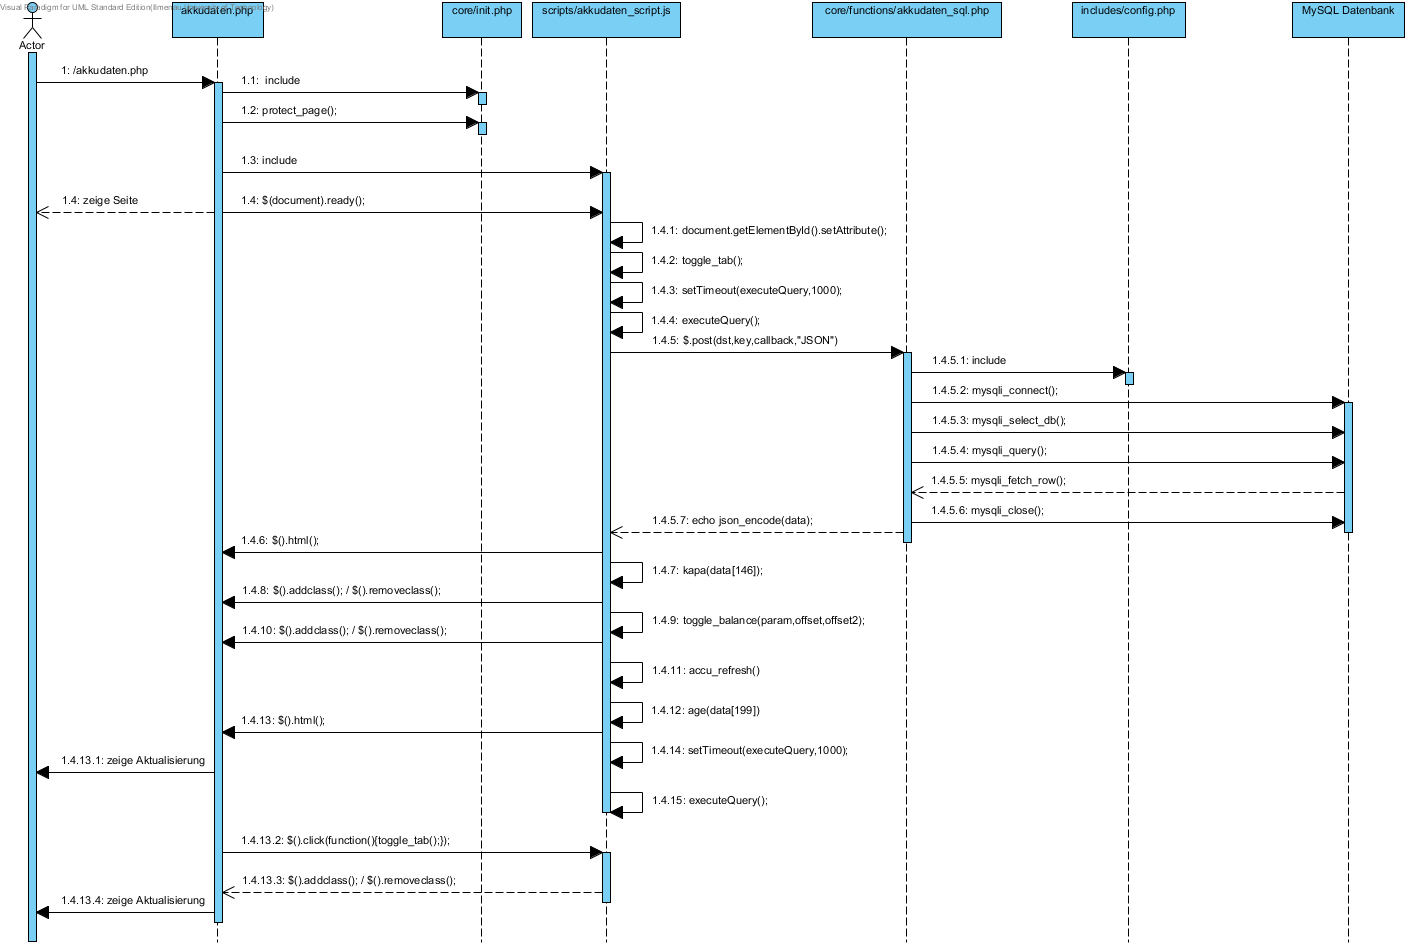
\includegraphics[scale=0.4255]{akkudatenvpp.png}
\\ \\ 
Die allgemeine Funktionsweise dieser Seite entspricht \textit{1.1.2. Allgemeine Fahrzeugdaten}. Im folgenden wird nur auf Besonderheiten dieser Seite eingegangen.\\

\textbf{accu\_refresh(data)}\\

\hangindent+95pt \hangafter=1 
Diese Funktion aktualisiert die 144 Zellspannungen und berechnet für die zwölf Akkublöcke jeweils minimale, sowie maximale Zellspannung. Der Funktion wird das JSON Array übergeben, dass in executeQuery() geholt wird. In diesem sind alle 144 Zellspannungen gespeichert.\\


\textbf{kapa(data[146],removeClass/addClass)}\\
\hangindent+95pt \hangafter=1 
Der Funktion wird der Wert der Gesamtspannung übergeben. Mit Hilfe dieses Wertes werden dann unter Nutzung von "'addclass/removeclass"' 10 Anzeigeflächen so eingefärbt, dass sie einen Wert zwischen 0 und 100 \% simulieren.\\

\textbf{toggle\_tab()}
\hspace{5.8mm}
\hangindent+95pt \hangafter=1 
Beim Seitenaufbau werden zuerst alle Tabellenspalten erstellt. Sobald der Seitenaufbau fertig ist, wird diese Funktion ausgeführt und versteckt alle Spalten, die sich auf Akkuzellen beziehen.\\

\textbf{toggle\_arrow()}
\hspace{1mm}
\hangindent+95pt \hangafter=1 
Dies ist eine Funktion, die "'toggle\_tab()"' zugeordnet ist. Sie sorgt dafür, das sich der visuelle Button zum Öffnen und Schließen nach dem Auslösen um $180^\circ$  dreht. Im Initialzustand zeigt der Pfeil nach unten und nach auslösen des Button dreht dieser sich und zeigt nach oben. Ein weiterer Klick macht den Vorgang rückgängig.\\


\textbf{toggle\_balance(), removeClass/addClass}\\
\hangindent+95pt \hangafter=1 
Analog wie in "'toggle\_notaus"' \textit{1.1.2. Allgemeine Fahrzeugdaten}. Hier wird der Ablauf für zwei Strings durchgeführt, die Balancing-Werte enthalten und bei Aktivität blau eingefärbt werden. Des weiteren wird an dieser Stelle auch gezählt, wie viele Zellen den Status "'AN"' haben. Die Anzahl wird in die Spalte des entsprechenden Akkublocks geschrieben und wenn diese größer als 0 ist ebenfalls blau hinterlegt.\\




\subsection{Dynamische Daten}
Der Aufbau ist wieder analog den vorherigen zwei Seiten. Auf dieser Seite wird folgendes visualisiert: 

\begin{itemize}
\item Drehzahlen der Räder als Halbkreis-Diagramm mit "'justGage"'
\item Die vier Federwege an den Achsen als vertikal stehender Ladebalken 
\item Gaspedal 1 und 2, Bremsposition, Bremskraft, Bremsdruck, Wassertemperatur 1 und 2 werden als horizontal liegender Ladebalken 
\item Der Lenkwinkel wird als Balken mit Indikator visualisiert.  
\end{itemize}

Auf der Seite wird die Draufsicht des Formula Student Fahrzeuges angezeigt, dass mit der Spitze nach oben zeigt. Darüber befindet sich die Visualisierung des Lenkwinkels und rechts, bzw. links befinden sich die Drehzahlanzeigen und die Federwege entsprechend der Achsen und Räder, die in der Fahrzeuggrafik zu sehen sind.
\\ \\
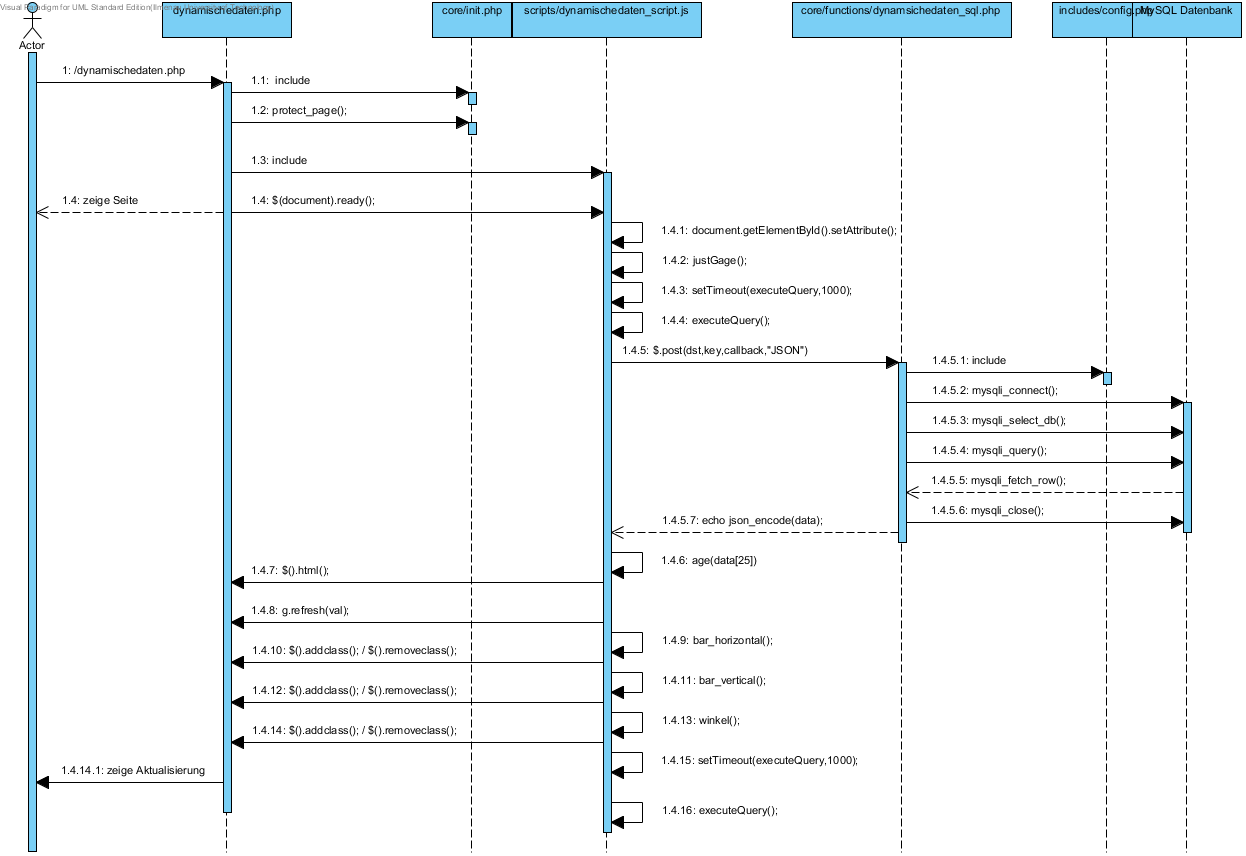
\includegraphics[scale=0.485]{dynamischedaten.png}
\\ \\
Bereits erwähnte Funktionen verhalten sich analog wie oben beschrieben.\\


\textbf{bar\_horizontal(), removeClass/addClass}\\
\hangindent+95pt \hangafter=1 
Bekommt als Eingabe eine ID und einen Wert. Danach wird mittels "'removeclass/addclass"' eine entsprechende Anzahl an Flächen farblich hinterlegt. Beschreibt eine horizontalen Ladebalken, der gefüllt wird.\\


\textbf{bar\_vertical(), removeClass/addClass}\\
\hangindent+95pt \hangafter=1 
Analog wie "'bar\_horizontal()"', nur das die Einfärbung der Flächen vertikal stattfindet.\\ 


\textbf{winkel(), removeClass/addClass}\\
\hangindent+95pt \hangafter=1
Rechnet den übergebenen Wert vom Wertebereich -180 bis +180 in den Wertebereich -90 bis +90. Danach wird genau eine Fläche eingefärbt, um den Grad des Lenkwinkels darzustellen.



\subsection{Fahrdynamik}
Aufbau der Seiten ist wieder analog den vorhergegangenen. Als Besonderheit auf der Seite ist nur, dass sie auf zwei Tabellen in der Datenbank zugreifen muss. Der Lenkwinkel ist nur in der Tabelle für dynamische Daten vorhanden, und muss deshalb extra abgefragt werden. Somit besteht die Seite im Prinzip aus vier Komponenten.\\ \\


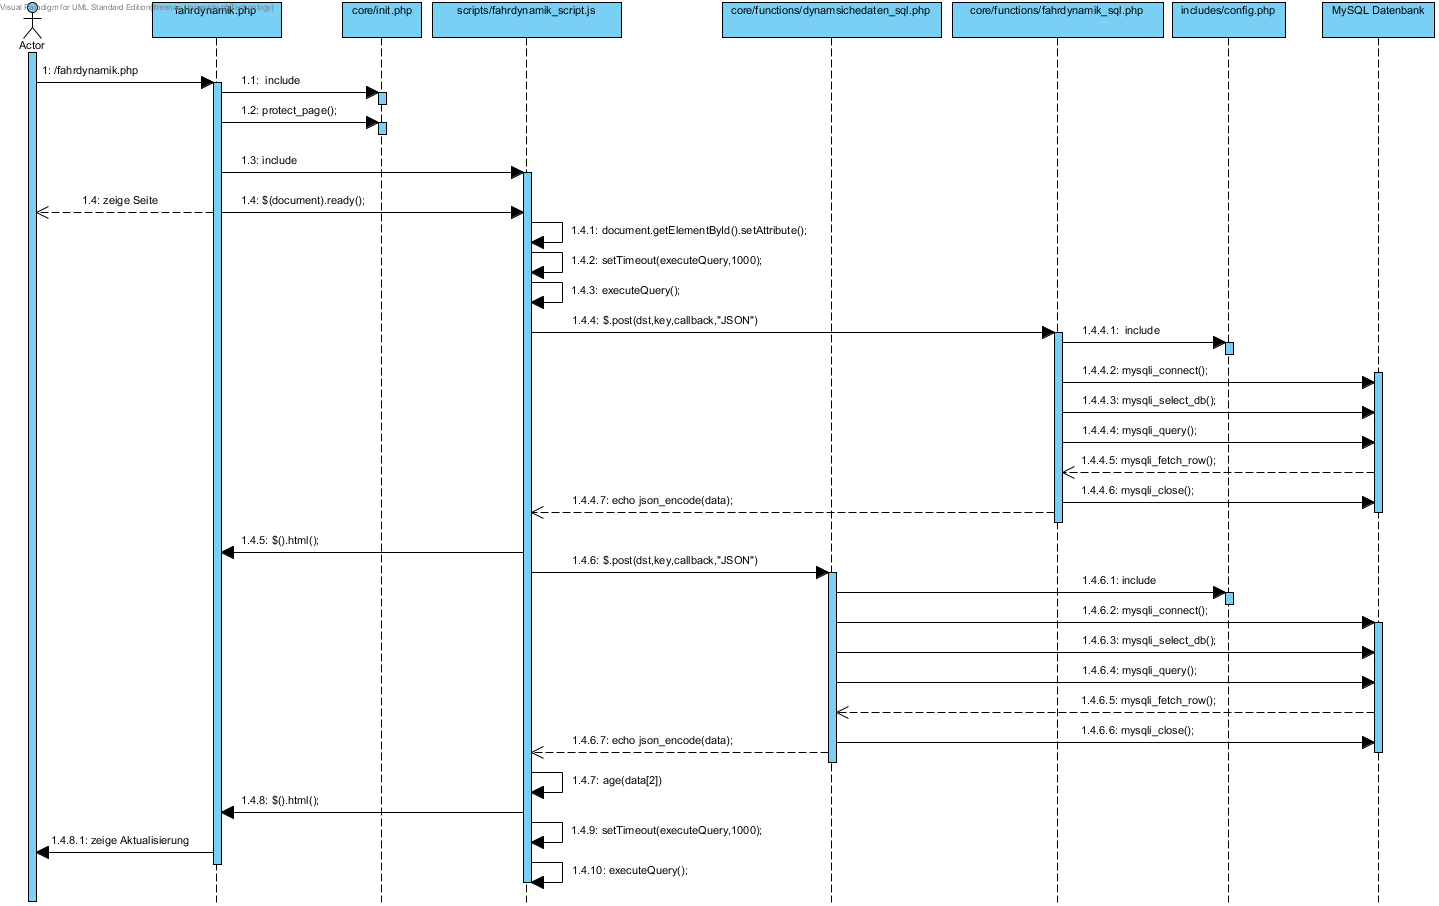
\includegraphics[scale=0.42]{fahrdynamik.png}
\\ \\
Funktionserklärung siehe vorhergegangene Seiten.\\



\subsection{Motor und Umrichter}
Diese Seite enthält die Daten, die im Pflichtenheft dafür vereinbart wurden und besteht wieder aus drei Komponenten. Die 8 Motortemperaturen werden als Tabelle dargestellt. Es gibt keine weiteren besonderen Merkmale auf dieser Seite.\\ \\



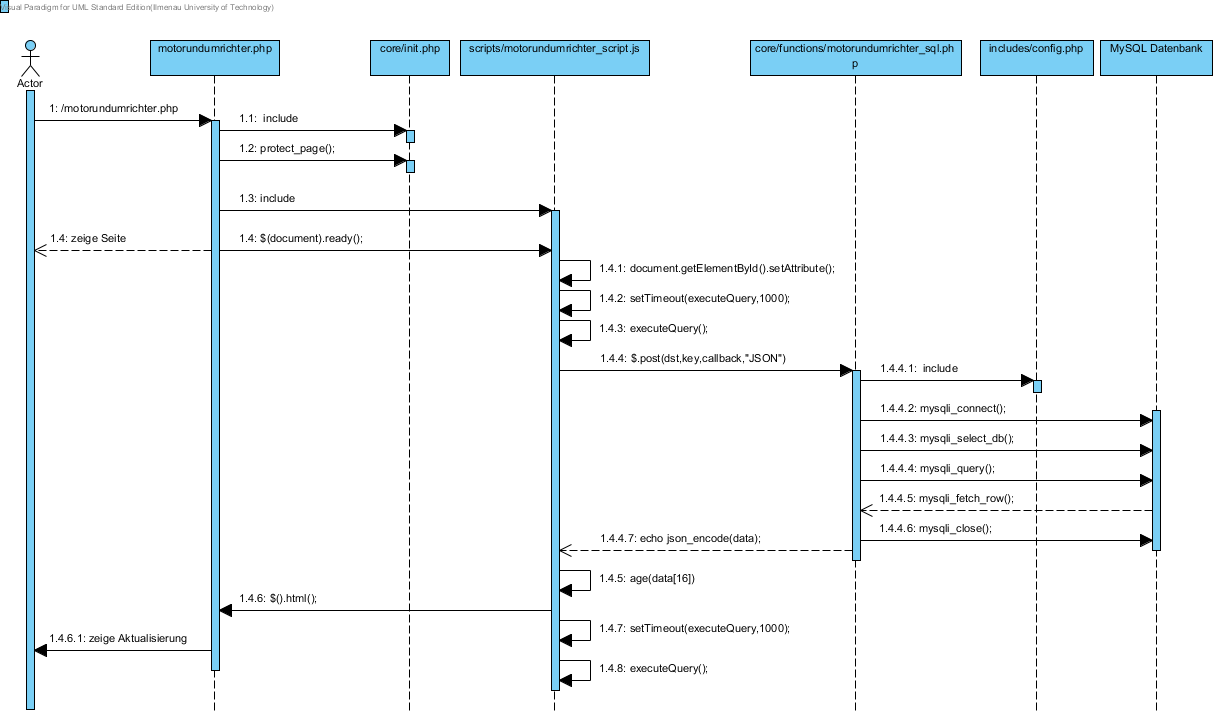
\includegraphics[scale=0.5]{motorundumrichter.png}
\\ \\
Funktion wie bereits oben erklärt.






%----------------------- Entwicklerdokumentation -------------------%

\chapter{Entwicklerdokumentation}



%------------------------- MicroAutoBox II -------------------------%

\section{MicroAutoBox II}

Da sich eine eigenständige Entwicklerdokumentation mittels doxygen oder anderen Softwarelösungen bei einem Simulink-Modell nicht anbietet, wurden bereits alle wesentlichen Informationen über das Modell im Feinentwurf unter Punkt 2.1 erläutert.

%--------------------------  Embedded PC  --------------------------%

\section{Embedded PC}

%--------------------------   vServer   ----------------------------%

\section{vServer}


%--------------------------   Webseite  ----------------------------%

\newpage

\section{Webseite}

Das Benutzersystem ermöglicht es nur bestimmten Personen auf Zugriff zur Seite zu gewähren. Hierbei gibt es die Möglichkeit sich persönlich zu registrieren und anschließend nach der Verifikation und Freischaltung durch den Vorstand (= Admin) sich auch einzuloggen. Im eingeloggten Zustand stehen dann Seiten zur Verfügung, die als nicht eingeloggter Benutzer nicht ersichtlich sind.\\

Im Folgenden sollen nun Funktionen und Variablen erläutert werden, sowie die Funktionalität der einzelnen Skripte des Systems.

\subsection{Allgemeine Funktionen (general.php)}
In dieser Datei befinden sich Funktionen, die nicht direkt mit dem aktiven Nutzer zu tun haben, sondern allgemein als (Hilfs-)Funktionen dienen.
\subsection*{install\_system(array \$register\_data)}
\subsubsection*{Author}
Thomas Golda
\subsubsection*{Beschreibung}
Diese Funktion dient dem Erstellen aller wichtigen Datenbanken, Tabellen und dem Anlegen eines Vorstand-Accounts, sowie dem Einrichten der Benutzergruppen 'Vorstand', 'Beobachter' und 'Techniker'. Das übergebene Array beinhaltet hierbei die für die Einrichtung des Vorstand-Accounts nötigen Benutzerinformationen.


\subsection*{logged\_in\_redirect()}
\subsubsection*{Author}
Thomas Golda
\subsubsection*{Beschreibung}
Dieser Funktion werden keine Parameter übergeben. Sie verwendet hierbei die Nutzerfunktion \textit{logged\_in()} und leitet einen Nutzer auf die Startseite weiter, wenn er bereits eingeloggt ist. Sie ist insbesondere dann nützlich, wenn man Seiten vor einem unsinnigen Zugriff des Nutzers schützen möchte. So macht es als eingeloggter Benutzer beispielsweise keinen Sinn das Registrierungsformular aufzurufen.


\subsection*{protect\_page()}
\subsubsection*{Author}
Thomas Golda
\subsubsection*{Beschreibung}
Diese Funktion arbeitet ähnlich zu \textit{logged\_in\_redirect()}, prüft ebenfalls durch Zuhilfenahme der Nutzerfunktion \textit{logged\_in()} ob sich ein aufrufender Nutzer bereits eingeloggt hat. Wenn dies nicht der Fall ist, wird er auf die Startseite weiter geleitet. Diese Funktion hilft insbesondere Seiten vor äußeren Zugriffen zu schützen.


\subsection*{array\_sanitize(array \$item)}
\subsubsection*{Author}
Thomas Golda
\subsubsection*{Beschreibung}
Diese Funktion erhält als Übergabe ein Array von Strings, die es mittels der PHP-internen Funktion \textit{mysqli\_real\_escape\_string()} aufbereitet um SQL-Injections beim Zugriff auf die Datenbank zu vermeiden.


\subsection*{sanitize(string \$data)}
\subsubsection*{Author}
Thomas Golda
\subsubsection*{Beschreibung}
Wie \textit{array\_sanitize()} wird auch hier der String von Sonderzeichen bereinigt. Der Unterschied: \textit{sanitize()} arbeitet auf einem einzelnen 
String.


\subsection*{output\_errors(array \$errors)}
\subsubsection*{Author}
Thomas Golda
\subsubsection*{Beschreibung}
Diese Funktion gibt alle auf einer Seite gesammelten benutzerdefinierten Fehlermeldungen in strukturierter Art und Weise wieder aus und weist den Benutzer somit darauf hin, dass ein Fehler (höchstwahrscheinlich) durch sein Verschulden entstanden ist. Er erhält auch zeitgleich eine Fehlermeldung die ihn darauf hinweist, wo sein Fehler liegt kann.

\newpage

% NUTZER FUNKTIONEN %

\subsection{Nutzerfunktionen (users.php)}
Die Funktionen in dieser Datei beziehen sich vorrangig auf den aktiven Benutzer und stellen Möglichkeiten dar auf seine Daten zuzugreifen oder mit diesen zu arbeiten.
\subsection*{change\_password(int \$user\_id, string \$password)}
\subsubsection*{Author}
Thomas Golda
\subsubsection*{Beschreibung}
Bekommt eine Nutzer-ID und einen String (= Passwort) übergeben. Das Passwort wird verschlüsselt und anschließend in der MySQL-Datenbank der Eintrag mit der ID \textit{\$user\_id} in der Benutzertabelle ermittelt. Für diesen Eintrag wird das alte Passwort durch das neue Passwort ersetzt.


\subsection*{register\_user(array \$register\_data)}
\subsubsection*{Author}
Thomas Golda
\subsubsection*{Beschreibung}
Diese Funktion bekommt ein Array von Strings übergeben und legt einen neuen Datenbankeintrag in der Tabelle für die Benutzer an.
Der neu angelegte Nutzer ist standardmäßig deaktiviert, hat somit nicht das Recht sich einzuloggen.


\subsection*{user\_count()}
\subsubsection*{Author}
Thomas Golda
\subsubsection*{Beschreibung}
Bestimmt die Anzahl der im System registrierten Benutzer. Nicht mit einberechnet werden noch nicht aktivierte Accounts.

\newpage

\subsection*{user\_data(int \$user\_id)}
\subsubsection*{Author}
Thomas Golda
\subsubsection*{Beschreibung}
Diese Funktion erfordert mindestens ein Argument und zwar die ID eines Nutzers. Wird sie mit mehr als diesem Parameter aufgerufen, so 
behandelt sich alle folgenden Parameter (vorzugsweise Strings) als gewünschte auszugebende Parameter.

% HIER SOLL DSA BILD REIN %
\begin{figure}[h]
\centering
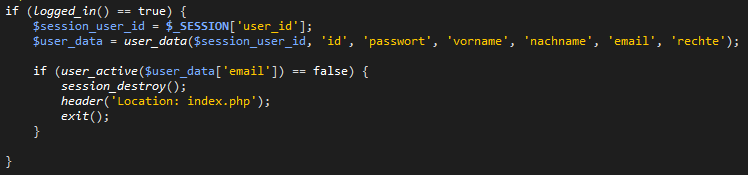
\includegraphics[scale = 0.78]{userdata.png}
\caption[user\_data() Funktion]{Quellcodeauszug aus \textit{core/init.php}}
\label{Quellcodeauszug aus core/init.php}
\end{figure}

Die Funktion selbst bestimmt zur übergebenen ID die weiterhin angegebenen Parameter und gibt diese als Array aus. So gibt die aus dem Bild ersichtliche aufgerufene Funktion, die zur ID gehörigen Daten wie Vor- und Nachname, E-Mail-Adresse, Rechtegruppe und das (verschlüsselte) Passwort.


\subsection*{isVorstand()}
\subsubsection*{Author}
Thomas Golda
\subsubsection*{Beschreibung}
Prüft ob der aktuell aktive Benutzer zur Rechtegruppe 'Vorstand' gehört oder nicht und gibt entweder \textit{true} oder \textit{false} zurück.


\subsection*{isTechniker()}
\subsubsection*{Author}
Thomas Golda
\subsubsection*{Beschreibung}
Prüft ob der aktuell aktive Benutzer zur Rechtegruppe 'Techniker' gehört oder nicht und gibt entweder \textit{true} oder \textit{false} zurück.


\subsection*{isBeobachter()}
\subsubsection*{Author}
Thomas Golda
\subsubsection*{Beschreibung}
Prüft ob der aktuell aktive Benutzer zur Rechtegruppe 'Beobachter' gehört oder nicht und gibt entweder \textit{true} oder \textit{false} zurück.


\subsection*{timeout()}
\subsubsection*{Author}
Thomas Golda
\subsubsection*{Beschreibung}
Überprüft ob der in der Session-Variable \textit{\$\_SESSION['time']} befindliche UNIX-Zeitstempel älter als \textit{\$time} Minuten ist. Standardwert: \textit{\$time} = 60.
Gibt \textit{true} zurück, falls der Zeitstempel nicht älter als \textit{\$time} Minuten ist, \textit{false} andernfalls.


\subsection*{logged\_in()}
\subsubsection*{Author}
Thomas Golda
\subsubsection*{Beschreibung}
Gibt zurück, ob der aktive Nutzer eingeloggt ist oder nicht. Dies impliziert auch eine Überprüfung ob seine letzte Aktivität weiter als eine in der Funktion \textit{timeout()} festgelegte Zeitspanne zurück liegt.
Setzt zudem nach dieser Prüfung den Zeitstempel in der Sessionvariable \textit{\$\_SESSION['time']} auf einen aktuellen Zeitwert.

\subsection*{refresh()}
\subsubsection*{Author}
Thomas Golda
\subsubsection*{Beschreibung}
Diese Funktioniert aktualisiert den Zeitwert in der Tabelle der Nutzer die sich zum aktuellen Zeitpunkt online befinden. Zudem werden alle veraltete Einträge unabhängig des Benutzers gelöscht.


\subsection*{user\_exists(string \$mail)}
\subsubsection*{Author}
Thomas Golda
\subsubsection*{Beschreibung}
Ermittelt mittels einer SQL-Anfrage ob der Benutzer der zur übermittelten E-Mail-Adresse \textit{\$mail} existiert oder nicht. Gibt im Erfolgsfall \textit{true}, sonst \textit{false} zurück.


\subsection*{user\_active(string \$mail)}
\subsubsection*{Author}
Thomas Golda
\subsubsection*{Beschreibung}
Gibt \textit{true} zurück, wenn der Nutzer mit der E-Mail-Adresse \textit{\$mail} bereits aktiviert wurde, \textit{false} sonst.


\subsection*{user\_id\_from\_mail(string \$mail)}
\subsubsection*{Author}
Thomas Golda
\subsubsection*{Beschreibung}
Bekommt als Argument einen String \textit{\$mail} (= E-Mail-Adresse). Ermittelt mittels einer SQL-Anfrage anschließend die ID des dazugehörigen Nutzers.


\subsection*{login(string \$mail, string \$password)}
\subsubsection*{Author}
Thomas Golda
\subsubsection*{Beschreibung}
Gibt bei Erfolg die Nutzer-ID des zugehörigen Nutzers zurück. Existiert kein Nutzer in der Datenbank mit den angegebenen Zugangsdaten, so gibt die Funktion \textit{false} zurück.

\newpage
\subsection{Konfigurationsdatei (config.php)}
Die Konfigurationsdatei wird stets in der core/init.php eingebunden und ist somit auf jeder Seite verfügbar, auf der auch init.php eingebunden wird. Inbesondere liefert sie die Zugangsdaten für den Zugriff auf die MySQL-Datenbanken und speichert auch die Namen der einzelnen Tabellen, sowohl für die Fahrzeugdaten, als auch für die Nutzerdaten.
\subsubsection*{\$dbhost}
Hier kann der Hostname des MySQL-Servers festgelegt werden. Er wird meist vom Hoster mitgeteilt und lautet in den meisten Fällen 'localhost'.
\subsubsection*{\$dbuname}
Hierbei handelt es sich um den Login-Namen der Zugangsdaten zum Datenbankserver. Diesen erhalten Sie ebenfalls von Ihrem Hoster.
\subsubsection*{\$dbpass}
Hierbei handelt es sich um das Passwort der Zugangsdaten zum Datenbankserver. Diesen erhalten Sie ebenfalls von Ihrem Hoster oder legen Sie selbst in Ihrer Serververwaltung fest.
\subsubsection*{\$dbname\_fd}
Hiermit legen Sie den Namen der Datenbank fest, in der die Tabellen der Fahrzeugdaten gespeichert werden sollen.
\subsubsection*{\$dbname\_ud}
Hiermit legen Sie den Namen der Datenbank fest, in der die Tabellen des Benutzersystems gespeichert werden sollen.
\subsubsection*{\$accu\_data}
Beinhaltet den Namen der Akkudaten-Tabelle.
\subsubsection*{\$general\_data}
Beinhaltet den Namen der Tabelle für die allgemeinen Fahrzeugdaten.
\subsubsection*{\$dynamic\_data}
Beinhaltet den Namen der Tabelle für die dynamischen Fahrzeugdaten.
\subsubsection*{\$engine\_data}
Beinhaltet den Namen der Tabelle für die Motor- und Umrichterdaten.
\subsubsection*{\$driving\_data}
Beinhaltet den Namen der Tabelle für die Fahrdynamikdaten.
\subsubsection*{\$user}
Beinhaltet den Namen der Tabelle der registrierten Benutzer.
\subsubsection*{\$rights}
Beinhaltet den Namen der Tabelle für die verschiedenen Rechtegruppen.
\subsubsection*{\$online}
Beinhaltet den Namen der Tabelle für die sich momentan online befindlichen Nutzer.
\subsubsection*{\$mail}
Beinhaltet die E-Mail-Adresse des Vorstands oder derjenigen Person, die Benutzer freischalten können soll. (Achtung: Funktionalität nicht implementiert!)
\subsubsection*{\$salt}
Ein Teil des Salt für das Passwort. Kann beliebiger String sein.
\subsubsection*{\$alg}
Ein Teil des Salt für das Passwort. Gibt den Verschlüsselungsalgorithmus an. (siehe Dokumentation der PHP-Funktion crypt())
\subsubsection*{\$rounds}
Ein Teil des Salt für das Passwort. Gibt die Anzahl der Runden an, die der Algorithmus laufen soll. Dabei gilt, je größer umso sicherer, aber auch aufwändiger und langsamer.
\subsubsection*{\$cryptsalt}
Endgültiger Salt. Setzt sich aus \$salt, \$alg und \$rounds zusammen.

\newpage
% RESTLICHE SEITEN %
\subsection{akkudaten.php}

\subsection{allgemeinefahrzeugdaten.php}

\subsection{changepassword.php}
Hierbei handelt es sich um eine Seite, die es dem Nutzer ermöglicht sein Passwort zu ändern. Durch Eingabe seines aktuellen Passwortes und der doppelten Eingabe seines neuen Passwortes wird eine SQL-Anfrage ausgeführt, die das alte Passwort in der Datenbank durch das neue Passwort überschreibt.
$\rightarrow$ Für weitere Informationen siehe Feinentwurfsdokument \glqq Passwort ändern\grqq (x.y.z)

\subsection{dynamischedaten.php}

\subsection{fahrdynamik.php}

\subsection{index.php}
Sie ist die Startseite des System und liefert im ausgeloggten Zustand die Möglichkeit sich mittels eines HTML-Formulares anzumelden bzw. im bereits eingeloggten Zustand sich verschiedene Widgets anzeigen zu lassen.
$\rightarrow$ Für weitere Informationen siehe Feinentwurfsdokument \glqq Startseite\grqq (x.y.z)

\subsection{install.php}
Diese Datei wird nur beim ersten Mal des Aufrufs der Seite gestartet. Sie bietet ein Formular, welches ausgefüllt werden muss und den ersten Benutzer im System erstellt: den Vorstand. Ihre Hauptaufgabe ist vor allem das Aufrufen der Funktion \textit{install\_system()} (siehe x.1.2).
$\rightarrow$ Für weitere Informationen siehe Feinentwurfsdokument \glqq Installation\grqq (x.y.z)

\subsection{login.php}
Bekommt Daten vom Formular der Startseite mittels POST-Request übermittelt. Diese werden verifiziert und nach erfolgreicher Verfikation ein Eintrag für die Online-Tabelle erstellt. Im Fehlerfall erhält der Nutzer eine Ausgabe über falsche bzw. fehlende Zugangsdaten. $\rightarrow$ Für weitere Informationen siehe Feinentwurfsdokument \glqq Login\grqq(x.y.z)

\subsection{logout.php}
Beendet die aktuelle Sitzung, löscht den zum aktiven Nutzer gehörigen Eintrag in der Online-Tabelle und leitet den Nutzer zurück auf die Startseite.
$\rightarrow$ Für weitere Informationen siehe Feinentwurfsdokument \glqq Logout\grqq (x.y.z)

\subsection{motorundumrichter.php}

\subsection{register.php}
Überprüft die bei der Registrierung eingegeben Daten und schreibt diese nach der Validierung in die Benutzertabelle der Datenbank. Das Passwort wird dabei verschlüsselt und gesalzen (Salt = \$cryptsalt siehe x.1.3) um es sicher zu speichern. Außerdem wird nach der Registrierung der Status des Accounts auf 0 gesetzt, d.h. er muss anschließend manuell aktiviert werden.
$\rightarrow$ Für weitere Informationen siehe Feinentwurfsdokument \glqq Registrierung\grqq (x.y.z)

\subsection{core/init.php}
Hierbei handelt es sich um eine Datei die zu Beginn jeder Inhaltsseite eingebunden wird. Sie wird insbesondere im Header eingebunden, welcher wiederum in jeder Inhaltsseite eingebunden wird und sorgt dafür, dass die Sitzung nach ihrer Erzeugung über jeden Seitenwechsel erhalten bleibt.
$\rightarrow$ Für weitere Informationen siehe Feinentwurfsdokument \glqq Initialisierung\grqq (x.y.z)

\subsection{core/functions/accept.php}
Erhält vom Widget \textit{includes/widgets/manageusers.php} per POST-Request Daten. Diese werden ausgewertet, d.h. es wird überprüft ob eine ID angegeben wurde und falls ja, diese von der eigenen verschieden ist. Desweiteren wird überprüft ob eine gewünschte Verwaltungsoption ('Löschen' bzw. 'Aktivieren') ausgewählt wurde, an sonsten wir der Nutzer zurück auf die Indexseite weitergeleitet. Abschließend wird noch die übergebene Rechtegruppe in einen Integer umgewandelt und mit den Daten anschließend eine Anfrage auf die Datenbank ausgeführt.
$\rightarrow$ Für weitere Informationen siehe Feinentwurfsdokument \glqq Benutzerverwaltung\grqq (x.y.z)

\subsection{core/functions/akkudaten\_sql.php}

\subsection{core/functions/allgemeinefahrzeugdaten\_sql.php}

\subsection{core/functions/csvexp\_sql.php}
Erhält vom Widget \textit{includes/widgets/csvexp.php} die Informationen welche Checkboxen vor Absenden des Formulars ausgewählt wurden als POST-Variablen. Diese Informationen werden ausgewertet und anschließend in eine SQL-Anfrage übersetzt die dann die gewünschten Daten ausgibt. Diese Daten werden dem Nutzer jedoch nicht im Browser dargestellt sondern als CSV-Datei zum Download angeboten.
$\rightarrow$ Für weitere Informationen siehe Feinentwurfsdokument \glqq CSV Export\grqq (x.y.z)

\subsection{core/functions/dynamischedaten\_sql.php}

\subsection{core/functions/fahrdynamik\_sql.php}

\subsection{core/functions/general.php}
Beinhaltet allgemeine (Hilfs-)Funktionen für das Benutzersystem.
$\rightarrow$ Ausführliche Beschreibung siehe x.1.1

\subsection{core/functions/motorundumrichter\_sql.php}

\subsection{core/functions/users.php}
Beinhaltet benutzerbezogene (Hilfs-)Funktionen für das Benutzersystem.
$\rightarrow$ Ausführliche Beschreibung siehe x.1.2

\subsection{includes/css/style.css}
Beinhaltet alle CSS-Formatierungen die auf der kompletten Seiten durchgeführt wurden. Für weitere Informationen siehe Kommentare in der Datei.

\subsection{includes/overall/footer.php}
Beinhaltet den globalen Footer, der auf jeder Inhaltsseite eingebunden wird.

\subsection{includes/overall/header.php}
Beinhaltet den globalen Header, der auf jeder Inhaltsseite eingebunden wird. Bindet zeitgleich auch die \textit{core/init.php} und \textit{includes/header.php} für die Darstellung des Menüs eins.

\subsection{includes/widgets/csvexp.php}
Hierbei handelt es sich um ein Widget, welches zur Auswahl der verschiedenen Fahrzeugdatentabellen jeweils eine Checkbox liefert und diese Daten nach einem Klick an die \textit{core/functions/csvexp\_sql.php} weiterleitet.
$\rightarrow$ Für weitere Informationen siehe Feinentwurfsdokument \glqq CSV Export\grqq (x.y.z)

\subsection{includes/widgets/loggedin.php}
Dies ist kein Widget wie es die anderen Dateien dieses Ordners sind. Es wird stets im Header eingebunden und liefert im eingeloggten Zustand eine namentliche Begrüßung des aktiven Nutzers. Desweiteren liefert es auf den einzeln Inhaltsseiten eine Information über das Alter der Daten. Außerdem gibt es einen Link zur \glqq Passwort ändern\grqq-Funktion sowie zur Startseite.

\subsection{includes/widgets/manageusers.php}
Dieses Widget erlaubt es im System registrierte Benutzer zu verwalten, d.h. sie zu aktivieren, zu löschen und ihnen eine Rechtegruppe zuzuweisen. Dies geschieht über ein Formular, dessen Daten über POST-Variablen an die \textit{core/functions/accept.php} weitergereicht werden.
$\rightarrow$ Für weitere Informationen siehe Feinentwurfsdokument \glqq Benutzerverwaltung\grqq (x.y.z)

\subsection{includes/widgets/onlineusers.php}
Ein weiteres Widget, welches die Benutzer als HTML-Tabelle ausgibt, die sich gerade eingeloggt im Benutzersystem befinden. Hierbei befindet sich bei jedem Nutzereintrag auch eine relative Zeitangabe seiner letzten Aktivität.

\subsection{includes/widgets/userlist.php}
Dieses Widget liefert über die \textit{includes/widgets/onlineusers.php} hinaus eine Liste aller im System registrierten Benutzer. Neben Vor- und Nachname werden auch E-Mail-Adresse, Rechtegruppe, Kontostatus und Online-Status ausgegeben.
$\rightarrow$ Für weitere Informationen siehe Feinentwurfsdokument \glqq Online Benutzer\grqq (x.y.z)



  









%----------------------  Abbildungsverzeichnis  --------------------%

\listoffigures

\addcontentsline{toc}{chapter}{Abbildungsverzeichnis}
%
%---------------------------  Anhang  ------------------------------%

%\addcontentsline{toc}{chapter}{Anhang}

\appendix
\addchap{Anhang} 
\refstepcounter{chapter}

\section{Simulink-Diagramme}

\begin{figure}[b]
\centering
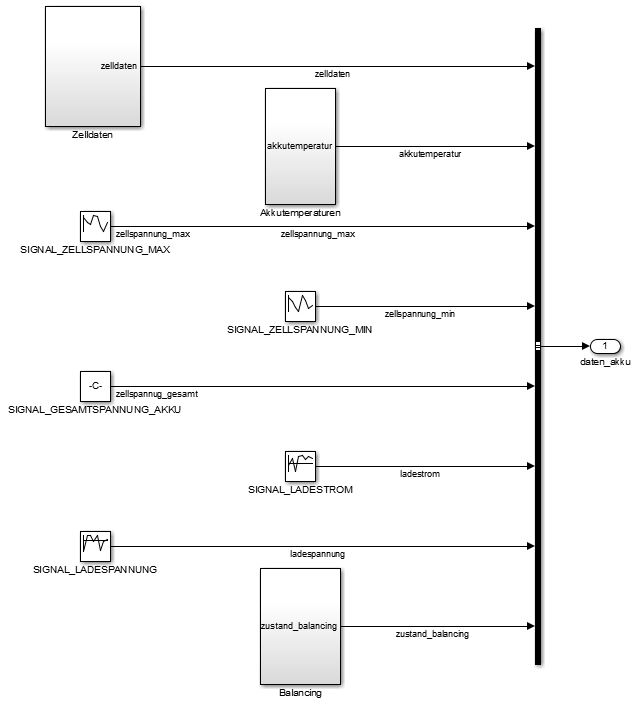
\includegraphics[scale = 0.8]{akkudaten}
\caption[Subsystem Akkudaten]{Subsystem Akkudaten}
\end{figure} 

\newpage


\begin{sidewaysfigure}[h]
\centering
\includegraphics[scale = 0.65]{zelldaten}
\caption[Subsystem Zelldaten]{Subsystem Zelldaten}
\end{sidewaysfigure} 

\newpage

\begin{figure}[h]
\centering
\includegraphics[scale = 0.85]{dyndaten}
\caption[Subsystem Dynamische Daten]{Übersicht über das Subsystem dynamische Daten}
\label{dyndaten}
\end{figure} 

\newpage

\begin{figure}[h]
\centering
\includegraphics[scale = 1]{submotordaten}
\caption[Subsystem Motor- und Umrichterdaten]{Übersicht über das Subsystem Motor- und Umrichterdaten}
\label{submotordaten}
\end{figure} 

\newpage

\begin{sidewaysfigure}[h]
\centering
\includegraphics[scale = 0.85]{subsignalkollektor}
\caption[Übersicht über das Subsystem Signalkollektor]{Übersicht über das Subsystem Signalkollektor}
\label{subsignalkollektor}
\end{sidewaysfigure}

\newpage

\begin{sidewaysfigure}[h]
\centering
\includegraphics[scale = 0.65]{sc_daten_notaus}
\caption[Übersicht über das Subsystem "`daten\_notaus"\ im Subsystem Allgemeine Fahrzeugdaten im Signalkollektor]{Übersicht über das Subsystem "`daten\_notaus"\ im Subsystem Allgemeine Fahrzeugdaten im Signalkollektor}
\label{scdatennotaus}
\end{sidewaysfigure}

\newpage

\begin{sidewaysfigure}[h]
\centering
\includegraphics[scale = 0.65]{sc_daten_temperatur_allgemein}
\caption[Übersicht über das Subsystem "`daten\_temperatur\_allgemein"\ im Subsystem Allgemeine Fahrzeugdaten im Signalkollektor]{Übersicht über das Subsystem "`daten\_temperatur\_allgemein"\ im Subsystem Allgemeine Fahrzeugdaten im Signalkollektor}
\label{scdatentemperaturallgemein}
\end{sidewaysfigure}

\newpage

\begin{figure}[h]
\centering
\includegraphics[scale = 0.8]{sc_daten_zellenpack}
\caption[Übersicht über das Subsystem "`daten\_zellenpack\_01"\ im Subsystem  "`daten\_zelldaten" im Signalkollektor]{Übersicht über das Subsystem "`daten\_zellenpack\_01"\ im Subsystem  "`daten\_zelldaten"\ im Signalkollektor}
\label{scdatenzellenpack}
\end{figure}


\newpage

\begin{figure}[h]
\centering
\includegraphics[scale = 0.85]{sc_daten_zelldaten}
\caption[Übersicht über das Subsystem "`daten\_zelldaten"\ im Subsystem  "`daten\_akku"\ im Signalkollektor]{Übersicht über das Subsystem "`daten\_zelldaten"\ im Subsystem  "`daten\_akku"\ im Signalkollektor}
\label{scdatenzelldaten}
\end{figure}

\newpage

\begin{figure}[h]
\centering
\includegraphics[scale = 0.77]{sc_daten_dynamisch}
\caption[Übersicht über das Subsystem "`daten\_dynamisch"\ im Signalkollektor]{Übersicht über das Subsystem "`daten\_dynamisch"\ im Signalkollektor}
\label{scdatendynamisch}
\end{figure}

\newpage

\begin{sidewaysfigure}[h]
\centering
\includegraphics[scale = 0.50]{subsignaltransmitter}
\caption[Übersicht über das Subsystem Signaltransmitter]{Übersicht über das Subsystem Signaltransmitter}
\label{subsignaltransmitter}
\end{sidewaysfigure}

\newpage

\begin{sidewaysfigure}[h]
\centering
\includegraphics[scale = 0.60]{subembreceive}
\caption[Übersicht über das Subsystem "`EMB\_RECEIVE"\ im Signaltransmitter]{Übersicht über das Subsystem "`EMB\_RECEIVE"\ im Signaltransmitter}
\label{subembreceive}
\end{sidewaysfigure}


\end{document}